% =============================================================================
% Modelo Matematico del Simulador QuadSIM-PRIMBIO -- 3ra edicion
% Compilar con docs/modelo/build.sh (xelatex x2). Los numeros que vienen de
% la verificacion numerica estan en valores.tex, generado por gen_valores.py
% a partir de resultados_verificacion.json (experiments/model_verification.py).
% =============================================================================
\documentclass[11pt,a4paper,oneside]{article}

\usepackage[spanish,provide=*]{babel}
\usepackage{unicode-math}
\setmainfont{Latin Modern Roman}
\setsansfont{Latin Modern Sans}
\setmonofont{Latin Modern Mono}[Scale=0.95]
\setmathfont{Latin Modern Math}

\usepackage[a4paper,top=2.6cm,bottom=2.6cm,left=2.7cm,right=2.5cm,headheight=14pt]{geometry}
\usepackage{amsmath,mathtools}
\usepackage{graphicx}
\usepackage{booktabs,tabularx,longtable,multirow,array}
\usepackage[table]{xcolor}
\usepackage{caption}
\usepackage{float}
\usepackage{enumitem}
\usepackage{microtype}
\usepackage{fancyhdr}
\usepackage{titlesec}
\usepackage[most]{tcolorbox}
\usepackage[hidelinks,unicode,bookmarksnumbered]{hyperref}
\usepackage[nameinlink,noabbrev]{cleveref}

\graphicspath{{figuras/}{../../experiments/results/benchmark_final/}}

% ---------------------------------------------------------------- colores
\definecolor{tinta}{HTML}{0B0B0B}
\definecolor{tinta2}{HTML}{52514E}
\definecolor{azul}{HTML}{2A78D6}
\definecolor{fondo}{HTML}{F3F6FB}
\definecolor{fondoN}{HTML}{FFF6EC}
\definecolor{naranja}{HTML}{EB6834}
\hypersetup{colorlinks=true,linkcolor=azul,citecolor=azul,urlcolor=azul}
\hypersetup{pdftitle={Modelo matemático del simulador QuadSIM-PRIMBIO, 3.ª edición},pdfauthor={Jesús Daniel Jácome; Francisco Javier Burgos Flórez (director)},pdfsubject={Proyecto Académico Especial, Semillero PRIMBIO, Grupo IAM-NANO, UNAL Sede La Paz}}

% ---------------------------------------------------------------- textos
\setlocalecaption{spanish}{table}{Tabla}
\setlocalecaption{spanish}{listtable}{Índice de tablas}
\captionsetup{font=small,labelfont=bf,margin=0.5cm}
\crefname{equation}{ecuación}{ecuaciones}
\Crefname{equation}{Ecuación}{Ecuaciones}
\crefname{figure}{figura}{figuras}
\Crefname{figure}{Figura}{Figuras}
\crefname{table}{tabla}{tablas}
\Crefname{table}{Tabla}{Tablas}
\crefname{section}{sección}{secciones}
\Crefname{section}{Sección}{Secciones}
\crefname{subsection}{sección}{secciones}
\Crefname{subsection}{Sección}{Secciones}
\creflabelformat{equation}{#2(#1)#3}
\newcommand{\crefpairconjunction}{ y }
\newcommand{\crefmiddleconjunction}{, }
\newcommand{\creflastconjunction}{ y }
\newcommand{\crefrangeconjunction}{ a }

\titleformat{\section}{\Large\bfseries\color{tinta}}{\thesection}{0.8em}{}
\titleformat{\subsection}{\large\bfseries\color{tinta}}{\thesubsection}{0.7em}{}
\titleformat{\subsubsection}{\normalsize\bfseries\color{tinta2}}{\thesubsubsection}{0.6em}{}
\numberwithin{equation}{section}
\numberwithin{figure}{section}
\numberwithin{table}{section}
\setlength{\parskip}{0.35em}
\setlength{\emergencystretch}{3em}
\setlength{\parindent}{0pt}
\setlist{itemsep=0.15em,topsep=0.3em}

\pagestyle{fancy}
\fancyhf{}
\fancyhead[L]{\small\color{tinta2}Modelo matemático del simulador QuadSIM-PRIMBIO --- 3.ª edición}
\fancyhead[R]{\small\color{tinta2}Sección~\thesection}
\fancyfoot[C]{\small\thepage}
\renewcommand{\headrulewidth}{0.4pt}

% ---------------------------------------------------------------- cajas
\newtcolorbox{nota}[1][]{enhanced,breakable,colback=fondo,colframe=azul,boxrule=0.5pt,
  left=6pt,right=6pt,top=4pt,bottom=4pt,arc=2pt,fonttitle=\bfseries\small,
  title={#1},coltitle=white}
\newtcolorbox{supuesto}[1][Supuesto]{enhanced,breakable,colback=fondoN,colframe=naranja,boxrule=0.5pt,
  left=6pt,right=6pt,top=4pt,bottom=4pt,arc=2pt,fonttitle=\bfseries\small,
  title={#1},coltitle=white}

% ---------------------------------------------------------------- notacion
\newcommand{\vect}[1]{\symbf{#1}}
\newcommand{\R}{\mathbf{R}}
\newcommand{\E}{\{E\}}
\newcommand{\B}{\{B\}}
\newcommand{\eu}{\vect{e}_3}
\newcommand{\sk}[1]{[#1]_{\times}}
\newcommand{\cod}[1]{\texttt{#1}}
\newcommand{\dif}{\mathrm{d}}
\newcommand{\T}{^{\mathsf{T}}}
\newcommand{\sat}{\operatorname{sat}}
\newcommand{\diag}{\operatorname{diag}}
\newcommand{\sgn}{\operatorname{sgn}}

% Generado por gen_valores.py -- NO EDITAR A MANO
\makeatletter
\@namedef{v@CPad}{0.0464}
\@namedef{v@CQad}{0.0074}
\@namedef{v@CTad}{0.110}
\@namedef{v@CmCt}{0.0161}
\@namedef{v@F15h}{1.1}
\@namedef{v@F15phi}{0.119}
\@namedef{v@F15rel}{0.8}
\@namedef{v@F15y}{2.7}
\@namedef{v@F15ymax}{2.05}
\@namedef{v@F2h}{0.0}
\@namedef{v@F2phi}{0.001}
\@namedef{v@F2rel}{0.1}
\@namedef{v@F2y}{0.1}
\@namedef{v@F2ymax}{0.28}
\@namedef{v@F30h}{4.5}
\@namedef{v@F30phi}{0.621}
\@namedef{v@F30rel}{2.1}
\@namedef{v@F30y}{11.3}
\@namedef{v@F30ymax}{4.18}
\@namedef{v@F5h}{0.1}
\@namedef{v@F5phi}{0.007}
\@namedef{v@F5rel}{0.1}
\@namedef{v@F5y}{0.7}
\@namedef{v@F5ymax}{0.69}
\@namedef{v@JmJz}{\ensuremath{3.33\times10^{-3}}}
\@namedef{v@KAxy}{1.023}
\@namedef{v@KP}{149.1}
\@namedef{v@KR}{147.8}
\@namedef{v@KY}{9.34}
\@namedef{v@Kmed1}{146.4}
\@namedef{v@Kmed2}{145.8}
\@namedef{v@KpNm}{0.753}
\@namedef{v@Kpred}{147.8}
\@namedef{v@Kt}{0.0104}
\@namedef{v@Qh}{0.0553}
\@namedef{v@Qmax}{0.180}
\@namedef{v@TW}{3.26}
\@namedef{v@Th}{3.432}
\@namedef{v@Tmax}{11.20}
\@namedef{v@Tmaxkgf}{1.14}
\@namedef{v@aDown}{7.85}
\@namedef{v@aUp}{17.75}
\@namedef{v@accLpf}{30}
\@namedef{v@alias}{179.6}
\@namedef{v@aliasMeas}{179.7}
\@namedef{v@atBWo}{-22.7}
\@namedef{v@atBWs}{-28.4}
\@namedef{v@atCH}{-21.3}
\@namedef{v@atLPc}{-35.9}
\@namedef{v@atNO}{-240.0}
\@namedef{v@axyMax}{5.66}
\@namedef{v@bancoComp}{$<0.05$~ms & 0.38~ms & 3.93~ms & 0.12~ms & 0.49~ms}
\@namedef{v@bancoN}{80}
\@namedef{v@bancoNTraj}{cuatro}
\@namedef{v@bancoRows}{Figura en 8 & nominal & 1.83 $\pm$ 0.28 & \textbf{1.50 $\pm$ 0.36} & 1.58 $\pm$ 0.41 & 4.56 $\pm$ 0.19 & 1.79 $\pm$ 0.37 \\
 & viento & 1.84 $\pm$ 0.44 & \textbf{1.66 $\pm$ 0.42} & 1.71 $\pm$ 0.46 & 5.36 $\pm$ 0.45 & 1.88 $\pm$ 0.44 \\
 & carga & 2.23 $\pm$ 0.28 & \textbf{1.85 $\pm$ 0.32} & 2.05 $\pm$ 0.37 & 4.66 $\pm$ 0.42 & 2.06 $\pm$ 0.29 \\
 & EMI & 5.90 $\pm$ 2.82 & \textbf{3.00 $\pm$ 0.14} & 3.03 $\pm$ 0.18 & 6.27 $\pm$ 0.09 & 3.13 $\pm$ 0.16 \\
\addlinespace[2pt]
Círculo & nominal & 1.59 $\pm$ 0.36 & \textbf{1.44 $\pm$ 0.39} & 1.52 $\pm$ 0.45 & 3.93 $\pm$ 0.26 & 1.77 $\pm$ 0.40 \\
 & viento & 1.80 $\pm$ 0.40 & \textbf{1.61 $\pm$ 0.36} & 1.65 $\pm$ 0.43 & 4.60 $\pm$ 0.70 & 1.85 $\pm$ 0.38 \\
 & carga & 1.98 $\pm$ 0.34 & \textbf{1.72 $\pm$ 0.36} & 1.96 $\pm$ 0.40 & 4.24 $\pm$ 0.49 & 1.99 $\pm$ 0.32 \\
 & EMI & 4.19 $\pm$ 1.80 & \textbf{1.81 $\pm$ 0.28} & 1.91 $\pm$ 0.31 & 3.48 $\pm$ 0.23 & 1.91 $\pm$ 0.33 \\
\addlinespace[2pt]
8 rápida & nominal & 6.22 $\pm$ 0.10 & \textbf{2.53 $\pm$ 0.24} & 2.87 $\pm$ 0.27 & 9.36 $\pm$ 0.23 & 3.07 $\pm$ 0.20 \\
 & viento & 5.54 $\pm$ 0.12 & \textbf{2.32 $\pm$ 0.27} & 2.62 $\pm$ 0.29 & 10.22 $\pm$ 0.48 & 2.74 $\pm$ 0.21 \\
 & carga & 7.28 $\pm$ 0.16 & \textbf{4.18 $\pm$ 0.29} & 4.22 $\pm$ 0.31 & 9.28 $\pm$ 0.25 & 4.46 $\pm$ 0.26 \\
 & EMI & 19.15 $\pm$ 2.90 & 16.27 $\pm$ 0.49 & \textbf{15.23 $\pm$ 0.41} & 139 $\pm$ 9 & 16.78 $\pm$ 0.50 \\
\addlinespace[2pt]
Escalones & nominal & 28.13 $\pm$ 0.20 & \textbf{8.87 $\pm$ 0.06} & 9.02 $\pm$ 0.07 & 20.88 $\pm$ 0.09 & 8.99 $\pm$ 0.05 \\
 & viento & 27.85 $\pm$ 0.23 & \textbf{8.94 $\pm$ 0.08} & 9.09 $\pm$ 0.10 & 21.07 $\pm$ 0.12 & 8.99 $\pm$ 0.07 \\
 & carga & 28.86 $\pm$ 0.25 & \textbf{9.32 $\pm$ 0.06} & 9.55 $\pm$ 0.08 & 21.09 $\pm$ 0.10 & 9.66 $\pm$ 0.05 \\
 & EMI & 133 $\pm$ 3 & \textbf{13.68 $\pm$ 0.44} & 14.90 $\pm$ 0.53 & 21.21 $\pm$ 0.12 & 14.50 $\pm$ 0.60 \\}
\@namedef{v@bancoSeedList}{1, 2 y 3}
\@namedef{v@bancoSeeds}{3}
\@namedef{v@bancoTrajList}{figura en 8, círculo, figura en 8 rápida y escalones en caja}
\@namedef{v@bancoVuelos}{240}
\@namedef{v@bestMpc}{15}
\@namedef{v@bestNmpc}{1}
\@namedef{v@bestPid}{0}
\@namedef{v@betaDef}{0.015}
\@namedef{v@bmpccirclemagemi}{1.81}
\@namedef{v@bmpccirclemagemieff}{0.036}
\@namedef{v@bmpccirclemagemimax}{3.54}
\@namedef{v@bmpccirclenominal}{1.44}
\@namedef{v@bmpccirclenominaleff}{0.033}
\@namedef{v@bmpccirclenominalmax}{2.55}
\@namedef{v@bmpccirclepayload}{1.72}
\@namedef{v@bmpccirclepayloadeff}{0.048}
\@namedef{v@bmpccirclepayloadmax}{4.97}
\@namedef{v@bmpccirclewind}{1.61}
\@namedef{v@bmpccirclewindeff}{0.038}
\@namedef{v@bmpccirclewindmax}{3.85}
\@namedef{v@bmpclemniscatefastmagemi}{16.27}
\@namedef{v@bmpclemniscatefastmagemieff}{0.104}
\@namedef{v@bmpclemniscatefastmagemimax}{28.26}
\@namedef{v@bmpclemniscatefastnominal}{2.53}
\@namedef{v@bmpclemniscatefastnominaleff}{0.089}
\@namedef{v@bmpclemniscatefastnominalmax}{4.24}
\@namedef{v@bmpclemniscatefastpayload}{4.18}
\@namedef{v@bmpclemniscatefastpayloadeff}{0.091}
\@namedef{v@bmpclemniscatefastpayloadmax}{7.86}
\@namedef{v@bmpclemniscatefastwind}{2.32}
\@namedef{v@bmpclemniscatefastwindeff}{0.095}
\@namedef{v@bmpclemniscatefastwindmax}{4.64}
\@namedef{v@bmpclemniscatemagemi}{3.00}
\@namedef{v@bmpclemniscatemagemieff}{0.038}
\@namedef{v@bmpclemniscatemagemimax}{5.95}
\@namedef{v@bmpclemniscatenominal}{1.50}
\@namedef{v@bmpclemniscatenominaleff}{0.036}
\@namedef{v@bmpclemniscatenominalmax}{2.69}
\@namedef{v@bmpclemniscatepayload}{1.85}
\@namedef{v@bmpclemniscatepayloadeff}{0.049}
\@namedef{v@bmpclemniscatepayloadmax}{4.72}
\@namedef{v@bmpclemniscatewind}{1.66}
\@namedef{v@bmpclemniscatewindeff}{0.043}
\@namedef{v@bmpclemniscatewindmax}{4.19}
\@namedef{v@bmpcrlcirclemagemi}{1.91}
\@namedef{v@bmpcrlcirclemagemieff}{0.034}
\@namedef{v@bmpcrlcirclemagemimax}{3.70}
\@namedef{v@bmpcrlcirclenominal}{1.77}
\@namedef{v@bmpcrlcirclenominaleff}{0.031}
\@namedef{v@bmpcrlcirclenominalmax}{3.07}
\@namedef{v@bmpcrlcirclepayload}{1.99}
\@namedef{v@bmpcrlcirclepayloadeff}{0.047}
\@namedef{v@bmpcrlcirclepayloadmax}{6.13}
\@namedef{v@bmpcrlcirclewind}{1.85}
\@namedef{v@bmpcrlcirclewindeff}{0.035}
\@namedef{v@bmpcrlcirclewindmax}{4.61}
\@namedef{v@bmpcrllemniscatefastmagemi}{16.78}
\@namedef{v@bmpcrllemniscatefastmagemieff}{0.096}
\@namedef{v@bmpcrllemniscatefastmagemimax}{29.34}
\@namedef{v@bmpcrllemniscatefastnominal}{3.07}
\@namedef{v@bmpcrllemniscatefastnominaleff}{0.083}
\@namedef{v@bmpcrllemniscatefastnominalmax}{5.20}
\@namedef{v@bmpcrllemniscatefastpayload}{4.46}
\@namedef{v@bmpcrllemniscatefastpayloadeff}{0.087}
\@namedef{v@bmpcrllemniscatefastpayloadmax}{8.08}
\@namedef{v@bmpcrllemniscatefastwind}{2.74}
\@namedef{v@bmpcrllemniscatefastwindeff}{0.087}
\@namedef{v@bmpcrllemniscatefastwindmax}{5.40}
\@namedef{v@bmpcrllemniscatemagemi}{3.13}
\@namedef{v@bmpcrllemniscatemagemieff}{0.036}
\@namedef{v@bmpcrllemniscatemagemimax}{6.41}
\@namedef{v@bmpcrllemniscatenominal}{1.79}
\@namedef{v@bmpcrllemniscatenominaleff}{0.034}
\@namedef{v@bmpcrllemniscatenominalmax}{3.06}
\@namedef{v@bmpcrllemniscatepayload}{2.06}
\@namedef{v@bmpcrllemniscatepayloadeff}{0.048}
\@namedef{v@bmpcrllemniscatepayloadmax}{5.94}
\@namedef{v@bmpcrllemniscatewind}{1.88}
\@namedef{v@bmpcrllemniscatewindeff}{0.041}
\@namedef{v@bmpcrllemniscatewindmax}{4.67}
\@namedef{v@bmpcrlstepwaypointsmagemi}{14.50}
\@namedef{v@bmpcrlstepwaypointsmagemieff}{0.186}
\@namedef{v@bmpcrlstepwaypointsmagemimax}{59.42}
\@namedef{v@bmpcrlstepwaypointsmagemios}{15.4}
\@namedef{v@bmpcrlstepwaypointsmagemiss}{3.2}
\@namedef{v@bmpcrlstepwaypointsmagemitr}{0.28}
\@namedef{v@bmpcrlstepwaypointsmagemits}{n/d}
\@namedef{v@bmpcrlstepwaypointsnominal}{8.99}
\@namedef{v@bmpcrlstepwaypointsnominaleff}{0.098}
\@namedef{v@bmpcrlstepwaypointsnominalmax}{52.36}
\@namedef{v@bmpcrlstepwaypointsnominalos}{9.5}
\@namedef{v@bmpcrlstepwaypointsnominalss}{0.6}
\@namedef{v@bmpcrlstepwaypointsnominaltr}{0.23}
\@namedef{v@bmpcrlstepwaypointsnominalts}{1.54}
\@namedef{v@bmpcrlstepwaypointspayload}{9.66}
\@namedef{v@bmpcrlstepwaypointspayloadeff}{0.101}
\@namedef{v@bmpcrlstepwaypointspayloadmax}{58.79}
\@namedef{v@bmpcrlstepwaypointspayloados}{14.9}
\@namedef{v@bmpcrlstepwaypointspayloadss}{0.6}
\@namedef{v@bmpcrlstepwaypointspayloadtr}{0.24}
\@namedef{v@bmpcrlstepwaypointspayloadts}{1.96}
\@namedef{v@bmpcrlstepwaypointswind}{8.99}
\@namedef{v@bmpcrlstepwaypointswindeff}{0.102}
\@namedef{v@bmpcrlstepwaypointswindmax}{50.46}
\@namedef{v@bmpcrlstepwaypointswindos}{8.4}
\@namedef{v@bmpcrlstepwaypointswindss}{0.7}
\@namedef{v@bmpcrlstepwaypointswindtr}{0.23}
\@namedef{v@bmpcrlstepwaypointswindts}{1.36}
\@namedef{v@bmpcstepwaypointsmagemi}{13.68}
\@namedef{v@bmpcstepwaypointsmagemieff}{0.171}
\@namedef{v@bmpcstepwaypointsmagemimax}{58.15}
\@namedef{v@bmpcstepwaypointsmagemios}{13.5}
\@namedef{v@bmpcstepwaypointsmagemiss}{3.4}
\@namedef{v@bmpcstepwaypointsmagemitr}{0.28}
\@namedef{v@bmpcstepwaypointsmagemits}{n/d}
\@namedef{v@bmpcstepwaypointsnominal}{8.87}
\@namedef{v@bmpcstepwaypointsnominaleff}{0.090}
\@namedef{v@bmpcstepwaypointsnominalmax}{50.79}
\@namedef{v@bmpcstepwaypointsnominalos}{6.9}
\@namedef{v@bmpcstepwaypointsnominalss}{0.5}
\@namedef{v@bmpcstepwaypointsnominaltr}{0.23}
\@namedef{v@bmpcstepwaypointsnominalts}{1.42}
\@namedef{v@bmpcstepwaypointspayload}{9.32}
\@namedef{v@bmpcstepwaypointspayloadeff}{0.092}
\@namedef{v@bmpcstepwaypointspayloadmax}{56.89}
\@namedef{v@bmpcstepwaypointspayloados}{11.5}
\@namedef{v@bmpcstepwaypointspayloadss}{0.5}
\@namedef{v@bmpcstepwaypointspayloadtr}{0.24}
\@namedef{v@bmpcstepwaypointspayloadts}{1.77}
\@namedef{v@bmpcstepwaypointswind}{8.94}
\@namedef{v@bmpcstepwaypointswindeff}{0.096}
\@namedef{v@bmpcstepwaypointswindmax}{50.92}
\@namedef{v@bmpcstepwaypointswindos}{6.9}
\@namedef{v@bmpcstepwaypointswindss}{0.6}
\@namedef{v@bmpcstepwaypointswindtr}{0.24}
\@namedef{v@bmpcstepwaypointswindts}{1.22}
\@namedef{v@bnmpccirclemagemi}{1.91}
\@namedef{v@bnmpccirclemagemieff}{0.048}
\@namedef{v@bnmpccirclemagemimax}{3.64}
\@namedef{v@bnmpccirclenominal}{1.52}
\@namedef{v@bnmpccirclenominaleff}{0.045}
\@namedef{v@bnmpccirclenominalmax}{2.67}
\@namedef{v@bnmpccirclepayload}{1.96}
\@namedef{v@bnmpccirclepayloadeff}{0.059}
\@namedef{v@bnmpccirclepayloadmax}{7.53}
\@namedef{v@bnmpccirclewind}{1.65}
\@namedef{v@bnmpccirclewindeff}{0.047}
\@namedef{v@bnmpccirclewindmax}{3.76}
\@namedef{v@bnmpclemniscatefastmagemi}{15.23}
\@namedef{v@bnmpclemniscatefastmagemieff}{0.110}
\@namedef{v@bnmpclemniscatefastmagemimax}{25.03}
\@namedef{v@bnmpclemniscatefastnominal}{2.87}
\@namedef{v@bnmpclemniscatefastnominaleff}{0.118}
\@namedef{v@bnmpclemniscatefastnominalmax}{4.78}
\@namedef{v@bnmpclemniscatefastpayload}{4.22}
\@namedef{v@bnmpclemniscatefastpayloadeff}{0.129}
\@namedef{v@bnmpclemniscatefastpayloadmax}{7.81}
\@namedef{v@bnmpclemniscatefastwind}{2.62}
\@namedef{v@bnmpclemniscatefastwindeff}{0.120}
\@namedef{v@bnmpclemniscatefastwindmax}{4.70}
\@namedef{v@bnmpclemniscatemagemi}{3.03}
\@namedef{v@bnmpclemniscatemagemieff}{0.050}
\@namedef{v@bnmpclemniscatemagemimax}{6.24}
\@namedef{v@bnmpclemniscatenominal}{1.58}
\@namedef{v@bnmpclemniscatenominaleff}{0.049}
\@namedef{v@bnmpclemniscatenominalmax}{2.79}
\@namedef{v@bnmpclemniscatepayload}{2.05}
\@namedef{v@bnmpclemniscatepayloadeff}{0.061}
\@namedef{v@bnmpclemniscatepayloadmax}{7.39}
\@namedef{v@bnmpclemniscatewind}{1.71}
\@namedef{v@bnmpclemniscatewindeff}{0.051}
\@namedef{v@bnmpclemniscatewindmax}{4.07}
\@namedef{v@bnmpcstepwaypointsmagemi}{14.90}
\@namedef{v@bnmpcstepwaypointsmagemieff}{0.218}
\@namedef{v@bnmpcstepwaypointsmagemimax}{64.70}
\@namedef{v@bnmpcstepwaypointsmagemios}{15.2}
\@namedef{v@bnmpcstepwaypointsmagemiss}{5.0}
\@namedef{v@bnmpcstepwaypointsmagemitr}{0.30}
\@namedef{v@bnmpcstepwaypointsmagemits}{n/d}
\@namedef{v@bnmpcstepwaypointsnominal}{9.02}
\@namedef{v@bnmpcstepwaypointsnominaleff}{0.138}
\@namedef{v@bnmpcstepwaypointsnominalmax}{51.10}
\@namedef{v@bnmpcstepwaypointsnominalos}{7.0}
\@namedef{v@bnmpcstepwaypointsnominalss}{0.5}
\@namedef{v@bnmpcstepwaypointsnominaltr}{0.24}
\@namedef{v@bnmpcstepwaypointsnominalts}{1.34}
\@namedef{v@bnmpcstepwaypointspayload}{9.55}
\@namedef{v@bnmpcstepwaypointspayloadeff}{0.157}
\@namedef{v@bnmpcstepwaypointspayloadmax}{55.70}
\@namedef{v@bnmpcstepwaypointspayloados}{13.8}
\@namedef{v@bnmpcstepwaypointspayloadss}{0.8}
\@namedef{v@bnmpcstepwaypointspayloadtr}{0.23}
\@namedef{v@bnmpcstepwaypointspayloadts}{1.96}
\@namedef{v@bnmpcstepwaypointswind}{9.09}
\@namedef{v@bnmpcstepwaypointswindeff}{0.137}
\@namedef{v@bnmpcstepwaypointswindmax}{50.85}
\@namedef{v@bnmpcstepwaypointswindos}{6.9}
\@namedef{v@bnmpcstepwaypointswindss}{0.6}
\@namedef{v@bnmpcstepwaypointswindtr}{0.24}
\@namedef{v@bnmpcstepwaypointswindts}{1.23}
\@namedef{v@bpidcirclemagemi}{4.19}
\@namedef{v@bpidcirclemagemieff}{0.027}
\@namedef{v@bpidcirclemagemimax}{8.39}
\@namedef{v@bpidcirclenominal}{1.59}
\@namedef{v@bpidcirclenominaleff}{0.018}
\@namedef{v@bpidcirclenominalmax}{2.96}
\@namedef{v@bpidcirclepayload}{1.98}
\@namedef{v@bpidcirclepayloadeff}{0.041}
\@namedef{v@bpidcirclepayloadmax}{6.25}
\@namedef{v@bpidcirclewind}{1.80}
\@namedef{v@bpidcirclewindeff}{0.021}
\@namedef{v@bpidcirclewindmax}{4.30}
\@namedef{v@bpidlemniscatefastmagemi}{19.15}
\@namedef{v@bpidlemniscatefastmagemieff}{0.089}
\@namedef{v@bpidlemniscatefastmagemimax}{38.99}
\@namedef{v@bpidlemniscatefastnominal}{6.22}
\@namedef{v@bpidlemniscatefastnominaleff}{0.058}
\@namedef{v@bpidlemniscatefastnominalmax}{10.16}
\@namedef{v@bpidlemniscatefastpayload}{7.28}
\@namedef{v@bpidlemniscatefastpayloadeff}{0.068}
\@namedef{v@bpidlemniscatefastpayloadmax}{12.11}
\@namedef{v@bpidlemniscatefastwind}{5.54}
\@namedef{v@bpidlemniscatefastwindeff}{0.062}
\@namedef{v@bpidlemniscatefastwindmax}{10.00}
\@namedef{v@bpidlemniscatemagemi}{5.90}
\@namedef{v@bpidlemniscatemagemieff}{0.033}
\@namedef{v@bpidlemniscatemagemimax}{12.59}
\@namedef{v@bpidlemniscatenominal}{1.83}
\@namedef{v@bpidlemniscatenominaleff}{0.020}
\@namedef{v@bpidlemniscatenominalmax}{3.58}
\@namedef{v@bpidlemniscatepayload}{2.23}
\@namedef{v@bpidlemniscatepayloadeff}{0.042}
\@namedef{v@bpidlemniscatepayloadmax}{6.04}
\@namedef{v@bpidlemniscatewind}{1.84}
\@namedef{v@bpidlemniscatewindeff}{0.024}
\@namedef{v@bpidlemniscatewindmax}{4.66}
\@namedef{v@bpidstepwaypointsmagemi}{133.44}
\@namedef{v@bpidstepwaypointsmagemieff}{0.170}
\@namedef{v@bpidstepwaypointsmagemimax}{217.65}
\@namedef{v@bpidstepwaypointsmagemios}{116.8}
\@namedef{v@bpidstepwaypointsmagemiss}{72.4}
\@namedef{v@bpidstepwaypointsmagemitr}{0.23}
\@namedef{v@bpidstepwaypointsmagemits}{n/d}
\@namedef{v@bpidstepwaypointsnominal}{28.13}
\@namedef{v@bpidstepwaypointsnominaleff}{0.100}
\@namedef{v@bpidstepwaypointsnominalmax}{101.26}
\@namedef{v@bpidstepwaypointsnominalos}{41.1}
\@namedef{v@bpidstepwaypointsnominalss}{3.8}
\@namedef{v@bpidstepwaypointsnominaltr}{0.42}
\@namedef{v@bpidstepwaypointsnominalts}{n/d}
\@namedef{v@bpidstepwaypointspayload}{28.86}
\@namedef{v@bpidstepwaypointspayloadeff}{0.103}
\@namedef{v@bpidstepwaypointspayloadmax}{101.42}
\@namedef{v@bpidstepwaypointspayloados}{41.4}
\@namedef{v@bpidstepwaypointspayloadss}{7.9}
\@namedef{v@bpidstepwaypointspayloadtr}{0.44}
\@namedef{v@bpidstepwaypointspayloadts}{n/d}
\@namedef{v@bpidstepwaypointswind}{27.85}
\@namedef{v@bpidstepwaypointswindeff}{0.131}
\@namedef{v@bpidstepwaypointswindmax}{100.26}
\@namedef{v@bpidstepwaypointswindos}{38.6}
\@namedef{v@bpidstepwaypointswindss}{3.6}
\@namedef{v@bpidstepwaypointswindtr}{0.43}
\@namedef{v@bpidstepwaypointswindts}{2.82}
\@namedef{v@brlcirclemagemi}{3.48}
\@namedef{v@brlcirclemagemieff}{0.046}
\@namedef{v@brlcirclemagemimax}{6.22}
\@namedef{v@brlcirclenominal}{3.93}
\@namedef{v@brlcirclenominaleff}{0.043}
\@namedef{v@brlcirclenominalmax}{5.98}
\@namedef{v@brlcirclepayload}{4.24}
\@namedef{v@brlcirclepayloadeff}{0.052}
\@namedef{v@brlcirclepayloadmax}{6.13}
\@namedef{v@brlcirclewind}{4.60}
\@namedef{v@brlcirclewindeff}{0.047}
\@namedef{v@brlcirclewindmax}{7.98}
\@namedef{v@brllemniscatefastmagemi}{138.91}
\@namedef{v@brllemniscatefastmagemieff}{0.187}
\@namedef{v@brllemniscatefastmagemimax}{334.15}
\@namedef{v@brllemniscatefastnominal}{9.36}
\@namedef{v@brllemniscatefastnominaleff}{0.067}
\@namedef{v@brllemniscatefastnominalmax}{14.52}
\@namedef{v@brllemniscatefastpayload}{9.28}
\@namedef{v@brllemniscatefastpayloadeff}{0.087}
\@namedef{v@brllemniscatefastpayloadmax}{15.14}
\@namedef{v@brllemniscatefastwind}{10.22}
\@namedef{v@brllemniscatefastwindeff}{0.068}
\@namedef{v@brllemniscatefastwindmax}{19.51}
\@namedef{v@brllemniscatemagemi}{6.27}
\@namedef{v@brllemniscatemagemieff}{0.042}
\@namedef{v@brllemniscatemagemimax}{10.37}
\@namedef{v@brllemniscatenominal}{4.56}
\@namedef{v@brllemniscatenominaleff}{0.040}
\@namedef{v@brllemniscatenominalmax}{7.83}
\@namedef{v@brllemniscatepayload}{4.66}
\@namedef{v@brllemniscatepayloadeff}{0.051}
\@namedef{v@brllemniscatepayloadmax}{8.19}
\@namedef{v@brllemniscatewind}{5.36}
\@namedef{v@brllemniscatewindeff}{0.044}
\@namedef{v@brllemniscatewindmax}{9.58}
\@namedef{v@brlstepwaypointsmagemi}{21.21}
\@namedef{v@brlstepwaypointsmagemieff}{0.241}
\@namedef{v@brlstepwaypointsmagemimax}{87.13}
\@namedef{v@brlstepwaypointsmagemios}{5.8}
\@namedef{v@brlstepwaypointsmagemiss}{5.1}
\@namedef{v@brlstepwaypointsmagemitr}{0.86}
\@namedef{v@brlstepwaypointsmagemits}{n/d}
\@namedef{v@brlstepwaypointsnominal}{20.88}
\@namedef{v@brlstepwaypointsnominaleff}{0.256}
\@namedef{v@brlstepwaypointsnominalmax}{87.17}
\@namedef{v@brlstepwaypointsnominalos}{2.5}
\@namedef{v@brlstepwaypointsnominalss}{2.1}
\@namedef{v@brlstepwaypointsnominaltr}{0.96}
\@namedef{v@brlstepwaypointsnominalts}{1.92}
\@namedef{v@brlstepwaypointspayload}{21.09}
\@namedef{v@brlstepwaypointspayloadeff}{0.233}
\@namedef{v@brlstepwaypointspayloadmax}{87.69}
\@namedef{v@brlstepwaypointspayloados}{2.6}
\@namedef{v@brlstepwaypointspayloadss}{2.3}
\@namedef{v@brlstepwaypointspayloadtr}{0.91}
\@namedef{v@brlstepwaypointspayloadts}{1.98}
\@namedef{v@brlstepwaypointswind}{21.07}
\@namedef{v@brlstepwaypointswindeff}{0.258}
\@namedef{v@brlstepwaypointswindmax}{88.08}
\@namedef{v@brlstepwaypointswindos}{2.6}
\@namedef{v@brlstepwaypointswindss}{2.3}
\@namedef{v@brlstepwaypointswindtr}{0.98}
\@namedef{v@brlstepwaypointswindts}{1.69}
\@namedef{v@catHead}{PAE-X450 & Jiřinec (+) & Luukkonen & KayLion & Hummingbird}
\@namedef{v@catRows}{PAE-X450 & X & 1.4 & 0.225 & 0.0241 / 0.0386 & \ensuremath{1.105\times10^{-5}} & \ensuremath{1.779\times10^{-7}} & 0.02 & 557 & 0.609 & 3.26 & 3.56 / 0.36 \\
Jiřinec (+) & + & 1.321 & 0.214 & 0.0093 / 0.0151 & \ensuremath{1.511\times10^{-5}} & \ensuremath{4.406\times10^{-7}} & 0.1 & 463 & 0.577 & 3.00 & 2.08 / 0.567 \\
Luukkonen & X & 0.468 & 0.225 & 0.00486 / 0.0088 & \ensuremath{2.980\times10^{-6}} & \ensuremath{1.140\times10^{-7}} & 0.05 & 620 & 0.577 & 3.00 & 1.1 / 0.263 \\
NUS KayLion & X & 0.032 & 0.058 & \ensuremath{3.07\times10^{-5}} / \ensuremath{5.97\times10^{-5}} & \ensuremath{3.334\times10^{-8}} & \ensuremath{1.058\times10^{-10}} & 0.0821 & 1534 & 0.707 & 2.00 & 0.0129 / 0.001 \\
AscTec Hummingbird & + & 0.5 & 0.175 & 0.00232 / 0.004 & \ensuremath{5.572\times10^{-6}} & \ensuremath{1.368\times10^{-7}} & 0.05 & 469 & 0.577 & 3.00 & 0.644 / 0.181 \\}
\@namedef{v@catT}{Bastidor & X & + & X & X & + \\
$m$ [kg] & 1.4 & 1.321 & 0.468 & 0.032 & 0.5 \\
$\ell$ [m] & 0.225 & 0.214 & 0.225 & 0.058 & 0.175 \\
$J_{xx}$ [kg·m$^2$] & 0.0241 & 0.0093 & 0.00486 & \ensuremath{3.07\times10^{-5}} & 0.00232 \\
$J_{zz}$ [kg·m$^2$] & 0.0386 & 0.0151 & 0.0088 & \ensuremath{5.97\times10^{-5}} & 0.004 \\
$C_T$ [N/(rad/s)$^2$] & \ensuremath{1.105\times10^{-5}} & \ensuremath{1.511\times10^{-5}} & \ensuremath{2.980\times10^{-6}} & \ensuremath{3.334\times10^{-8}} & \ensuremath{5.572\times10^{-6}} \\
$C_M$ [N·m/(rad/s)$^2$] & \ensuremath{1.779\times10^{-7}} & \ensuremath{4.406\times10^{-7}} & \ensuremath{1.140\times10^{-7}} & \ensuremath{1.058\times10^{-10}} & \ensuremath{1.368\times10^{-7}} \\
$T_m$ [s] & 0.02 & 0.1 & 0.05 & 0.0821 & 0.05 \\
$\Omega_h$ [rad/s] & 557 & 463 & 620 & 1534 & 469 \\
$\sigma_h$ & 0.609 & 0.577 & 0.577 & 0.707 & 0.577 \\
Empuje/peso & 3.26 & 3.00 & 3.00 & 2.00 & 3.00 \\
$\tau_{x,max}$ [N·m] & 3.56 & 2.08 & 1.1 & 0.0129 & 0.644 \\
$\tau_{z,max}$ [N·m] & 0.36 & 0.567 & 0.263 & 0.001 & 0.181 \\}
\@namedef{v@chQ}{0.957}
\@namedef{v@cirA}{0.61}
\@namedef{v@cirDur}{23.0}
\@namedef{v@cirTilt}{3.6}
\@namedef{v@cirV}{0.94}
\@namedef{v@clEumilphi}{\ensuremath{1.1\times10^{-1}}}
\@namedef{v@clEumily}{\ensuremath{3.0\times10^{-3}}}
\@namedef{v@clEuquiphi}{\ensuremath{2.3\times10^{-1}}}
\@namedef{v@clEuquiy}{\ensuremath{6.1\times10^{-3}}}
\@namedef{v@clRKmilphi}{\ensuremath{1.4\times10^{-7}}}
\@namedef{v@clRKmily}{\ensuremath{7.0\times10^{-9}}}
\@namedef{v@clRKquiphi}{\ensuremath{2.6\times10^{-5}}}
\@namedef{v@clRKquiy}{\ensuremath{1.1\times10^{-6}}}
\@namedef{v@condB}{62.1}
\@namedef{v@cross}{\ensuremath{1.6\times10^{-7}}}
\@namedef{v@ctrlHz}{500}
\@namedef{v@dBaro}{15}
\@namedef{v@dImu}{1}
\@namedef{v@dOm}{22463}
\@namedef{v@dPos}{5}
\@namedef{v@defAt}{-28.4}
\@namedef{v@defGd10}{3.67}
\@namedef{v@defGd20}{3.96}
\@namedef{v@desatKy}{0.00}
\@namedef{v@desatShift}{-14.38}
\@namedef{v@desatSig}{0.472, 1.000, 1.000, 0.472}
\@namedef{v@desatT}{25.93}
\@namedef{v@desatTx}{3.00}
\@namedef{v@dpdO}{0.08131}
\@namedef{v@drdO}{0.005137}
\@namedef{v@driftV}{\ensuremath{1.8\times10^{-14}}}
\@namedef{v@dryL}{11.66}
\@namedef{v@dryRatio}{0.505}
\@namedef{v@drySu}{0.968}
\@namedef{v@drySw}{0.500}
\@namedef{v@dryTc}{3.89}
\@namedef{v@dryTm}{3.75}
\@namedef{v@dvzdO}{\ensuremath{-8.7979\times10^{-3}}}
\@namedef{v@dzEst}{8.53}
\@namedef{v@dzFirst}{7.87}
\@namedef{v@dzFlips}{3}
\@namedef{v@dzLam}{1.121}
\@namedef{v@eBinv}{\ensuremath{5.9\times10^{-16}}}
\@namedef{v@eJac}{\ensuremath{8.7\times10^{-9}}}
\@namedef{v@eOrth}{\ensuremath{1.6\times10^{-15}}}
\@namedef{v@eRound}{\ensuremath{1.3\times10^{-15}}}
\@namedef{v@eW}{\ensuremath{8.9\times10^{-10}}}
\@namedef{v@eZYX}{\ensuremath{8.9\times10^{-16}}}
\@namedef{v@eigMin}{-50.000}
\@namedef{v@ekfAcc}{0.5}
\@namedef{v@ekfBias}{0.0002}
\@namedef{v@ekfGyro}{0.02}
\@namedef{v@ekfMag}{0.3}
\@namedef{v@emiH}{7.12}
\@namedef{v@emiPsi}{10.3}
\@namedef{v@emiRel}{26}
\@namedef{v@errEu2ms}{\ensuremath{1.9\times10^{-2}}}
\@namedef{v@errRK1ms}{\ensuremath{1.6\times10^{-10}}}
\@namedef{v@errRKfloor}{\ensuremath{5.2\times10^{-12}}}
\@namedef{v@estDef}{Mahony}
\@namedef{v@fastGain}{59}
\@namedef{v@fbp}{177.4}
\@namedef{v@fbpmax}{320.4}
\@namedef{v@filtroDef}{Butterworth de 60~Hz}
\@namedef{v@filtroDefFc}{60}
\@namedef{v@flatPitch}{-5.82}
\@namedef{v@flatRoll}{11.53}
\@namedef{v@flatT}{13.80}
\@namedef{v@fracTm}{0.641}
\@namedef{v@freeEuE}{\ensuremath{6.0\times10^{-3}}}
\@namedef{v@freeEuL}{\ensuremath{3.1\times10^{-3}}}
\@namedef{v@freeRKE}{\ensuremath{2.7\times10^{-14}}}
\@namedef{v@freeRKL}{\ensuremath{2.4\times10^{-11}}}
\@namedef{v@fvib}{177.4}
\@namedef{v@gdBWo}{2.62}
\@namedef{v@gdBWs}{3.67}
\@namedef{v@gdCH}{1.84}
\@namedef{v@gdLPc}{5.84}
\@namedef{v@gdNO}{0.12}
\@namedef{v@gea}{1.333}
\@namedef{v@geb}{1.067}
\@namedef{v@gec}{1.016}
\@namedef{v@ged}{1.004}
\@namedef{v@gee}{1.001}
\@namedef{v@hbkF}{\ensuremath{5.5717\times10^{-6}}}
\@namedef{v@hbkM}{\ensuremath{1.3678\times10^{-7}}}
\@namedef{v@hekfNp}{0.01 / 0.13}
\@namedef{v@hekfNr}{0.53 / 0.13}
\@namedef{v@hekfNy}{0.31 / 0.03}
\@namedef{v@hekfVp}{0.00 / 0.13}
\@namedef{v@hekfVr}{0.53 / 0.13}
\@namedef{v@hekfVy}{0.31 / 0.03}
\@namedef{v@hmadNp}{0.21 / 0.05}
\@namedef{v@hmadNr}{0.68 / 0.06}
\@namedef{v@hmadNy}{0.43 / 0.02}
\@namedef{v@hmadVp}{0.21 / 0.05}
\@namedef{v@hmadVr}{0.68 / 0.06}
\@namedef{v@hmadVy}{0.43 / 0.02}
\@namedef{v@hmahNp}{0.10 / 0.06}
\@namedef{v@hmahNr}{0.62 / 0.06}
\@namedef{v@hmahNy}{0.42 / 0.04}
\@namedef{v@hmahVp}{0.10 / 0.06}
\@namedef{v@hmahVr}{0.62 / 0.06}
\@namedef{v@hmahVy}{0.42 / 0.04}
\@namedef{v@jirM}{1.3216}
\@namedef{v@jirW}{489.1}
\@namedef{v@kdFactor}{1.00}
\@namedef{v@kdPitch}{0.00335}
\@namedef{v@kdRoll}{0.00338}
\@namedef{v@kiRatePitch}{1.6378}
\@namedef{v@kiRateRoll}{1.6515}
\@namedef{v@kiRateYaw}{26.140}
\@namedef{v@kpAng}{7.812}
\@namedef{v@kpRatePitch}{0.2096}
\@namedef{v@kpRateRoll}{0.2114}
\@namedef{v@kpRateYaw}{3.3459}
\@namedef{v@lemA}{0.99}
\@namedef{v@lemDur}{23.0}
\@namedef{v@lemRA}{3.95}
\@namedef{v@lemRDur}{18.0}
\@namedef{v@lemRTilt}{21.9}
\@namedef{v@lemRV}{2.81}
\@namedef{v@lemTilt}{5.7}
\@namedef{v@lemV}{1.40}
\@namedef{v@lostSentence}{En la figura en 8 rápida con interferencia magnética pierde la trayectoria (error máximo por encima de 1~m) el RL puro en todas las semillas. El de menor RMSE medio ahí es el NMPC, con 15.2~cm.}
\@namedef{v@lowShift}{2.17}
\@namedef{v@lowSig}{0.000, 0.588, 0.588, 0.000}
\@namedef{v@lowT}{6.29}
\@namedef{v@lowTx}{1.00}
\@namedef{v@magD}{18.53}
\@namedef{v@magDecl}{-9.85}
\@namedef{v@magE}{-4.63}
\@namedef{v@magF}{32.8}
\@namedef{v@magI}{34.4}
\@namedef{v@magN}{26.66}
\@namedef{v@mahKi}{0.05}
\@namedef{v@mahKp}{1}
\@namedef{v@mekfCe}{0.8}
\@namedef{v@mekfCr}{14.2}
\@namedef{v@mekfSe}{15.4}
\@namedef{v@mekfSr}{30.3}
\@namedef{v@minVb}{\ensuremath{9.9\times10^{-6}}}
\@namedef{v@mmadCe}{0.8}
\@namedef{v@mmadCr}{14.3}
\@namedef{v@mmadSe}{2.2}
\@namedef{v@mmadSr}{17.0}
\@namedef{v@mmahCe}{0.8}
\@namedef{v@mmahCr}{14.3}
\@namedef{v@mmahSe}{21.5}
\@namedef{v@mmahSr}{36.2}
\@namedef{v@mpcCond}{112}
\@namedef{v@mpcInv}{\ensuremath{2.1\times10^{-14}}}
\@namedef{v@mpcKax}{0.946}
\@namedef{v@mpcKaz}{0.252}
\@namedef{v@mpcKvx}{11.80}
\@namedef{v@mpcKvz}{14.00}
\@namedef{v@mpcKx}{35.8}
\@namedef{v@mpcKz}{42.4}
\@namedef{v@msA}{2.25}
\@namedef{v@msCost}{172.3}
\@namedef{v@msDur}{12.1}
\@namedef{v@msJump}{\ensuremath{6.6\times10^{-15}}}
\@namedef{v@msTilt}{12.7}
\@namedef{v@msV}{1.67}
\@namedef{v@nCombos}{16}
\@namedef{v@navBaro}{308}
\@namedef{v@navPos}{3000}
\@namedef{v@nmpcCost}{10}
\@namedef{v@nmpcThi}{38.57}
\@namedef{v@nmpcTlo}{2.75}
\@namedef{v@notchDef}{apagado}
\@namedef{v@notchQ}{2}
\@namedef{v@nouter}{5}
\@namedef{v@nsub}{2}
\@namedef{v@ordEuler}{1.00}
\@namedef{v@ordRK}{4.19}
\@namedef{v@ordRKpares}{4.07, 3.87, 4.62, 4.16}
\@namedef{v@outerHz}{100}
\@namedef{v@pairMpcNmpcRows}{13}
\@namedef{v@pairMpcPid}{48}
\@namedef{v@pairMpcrlWorse}{48}
\@namedef{v@pairTotal}{48}
\@namedef{v@pdkixy}{3.32}
\@namedef{v@pdkiz}{16.13}
\@namedef{v@pdkpxy}{1.21}
\@namedef{v@pdkpz}{2.68}
\@namedef{v@pdkvxy}{3.64}
\@namedef{v@pdkvz}{8.03}
\@namedef{v@phBWo}{-9.3}
\@namedef{v@phBWs}{-13.0}
\@namedef{v@phCH}{-6.5}
\@namedef{v@phLPc}{-20.2}
\@namedef{v@phNO}{-0.4}
\@namedef{v@physHz}{1000}
\@namedef{v@pidKiDef}{2}
\@namedef{v@pidKpDef}{3.6}
\@namedef{v@pidKvDef}{5.5}
\@namedef{v@plCMz}{8.82}
\@namedef{v@plJx}{0.02410, 0.02452, 0.03922}
\@namedef{v@plJz}{0.02472, 0.02452, 0.03860}
\@namedef{v@plMy}{-0.147}
\@namedef{v@plSig}{0.658}
\@namedef{v@plU}{-0.041}
\@namedef{v@psdPeak}{177.2}
\@namedef{v@reac}{2.89}
\@namedef{v@reacRatio}{19}
\@namedef{v@reacRatioAero}{16}
\@namedef{v@rectBound}{0.67}
\@namedef{v@rectekfC}{0.63}
\@namedef{v@rectekfCmax}{0.87}
\@namedef{v@rectekfF}{0.48}
\@namedef{v@rectekfFmax}{0.69}
\@namedef{v@rectmadC}{1.26}
\@namedef{v@rectmadCmax}{1.93}
\@namedef{v@rectmadF}{0.54}
\@namedef{v@rectmadFmax}{0.70}
\@namedef{v@rectmahC}{0.52}
\@namedef{v@rectmahCmax}{0.68}
\@namedef{v@rectmahF}{0.51}
\@namedef{v@rectmahFmax}{0.67}
\@namedef{v@reidRmseFO}{8.6}
\@namedef{v@reidRmseFOPDT}{3.6}
\@namedef{v@reidTau}{117.2}
\@namedef{v@reidTauF}{56.1}
\@namedef{v@reidThF}{49}
\@namedef{v@resHover}{\ensuremath{5.7\times10^{-12}}}
\@namedef{v@resMax}{23}
\@namedef{v@resMin}{0.5}
\@namedef{v@resNeg}{0}
\@namedef{v@rlBeatsPid}{cinco}
\@namedef{v@rlBeatsPidList}{círculo con interferencia magnética; escalones en caja en los cuatro escenarios}
\@namedef{v@rlRatioMax}{4.40}
\@namedef{v@rlRatioMin}{1.55}
\@namedef{v@rlRatioRows}{las 15 filas en que ni el RL puro ni el MPC pierden la trayectoria}
\@namedef{v@rlRatioSeedMax}{4.6}
\@namedef{v@rlRatioSmMax}{4.40}
\@namedef{v@rlRatioSmMin}{2.22}
\@namedef{v@rmsFilt}{0.32}
\@namedef{v@rmsRaw}{1.58}
\@namedef{v@rmseFO}{7.5}
\@namedef{v@rmseFOPDT}{3.1}
\@namedef{v@rmseZ}{0.6}
\@namedef{v@rtf}{13.5}
\@namedef{v@sgAcc}{0.0093}
\@namedef{v@sgAccmg}{0.95}
\@namedef{v@sgGyro}{0.079}
\@namedef{v@sigNyq}{0.807}
\@namedef{v@sigmah}{0.6087}
\@namedef{v@sigmahd}{0.609}
\@namedef{v@sigpitch}{0.6304, 0.5859, 0.6304, 0.5859}
\@namedef{v@sigroll}{0.5859, 0.6304, 0.6304, 0.5859}
\@namedef{v@sigyaw}{0.6608, 0.6608, 0.5502, 0.5502}
\@namedef{v@stabY}{\ensuremath{1.1\times10^{-2}}}
\@namedef{v@stabZ}{\ensuremath{1.4\times10^{-3}}}
\@namedef{v@stepErr}{\ensuremath{1.8\times10^{-3}}}
\@namedef{v@stepOS}{0.00}
\@namedef{v@stepRise}{130}
\@namedef{v@tauAtt}{117.2}
\@namedef{v@tauAttF}{59.8}
\@namedef{v@tauAxy}{119.1}
\@namedef{v@tauAxyF}{61.8}
\@namedef{v@tauAz}{19.5}
\@namedef{v@tauRY}{9.9}
\@namedef{v@taumaxR}{3.563}
\@namedef{v@taumaxY}{0.361}
\@namedef{v@taumot}{0.156}
\@namedef{v@thAttF}{43}
\@namedef{v@thAxyF}{43}
\@namedef{v@theta}{16}
\@namedef{v@tiltMax}{30}
\@namedef{v@vKiVel}{8.163}
\@namedef{v@vKpPos}{1.429}
\@namedef{v@vKpVel}{5.714}
\@namedef{v@wNyq}{785.4}
\@namedef{v@wc}{31.25}
\@namedef{v@wh}{557.3}
\@namedef{v@whrpm}{5322}
\@namedef{v@wmax}{1006.6}
\@namedef{v@wmaxrpm}{9612}
\@namedef{v@zBaro}{2.61}
\@namedef{v@zNoBaro}{2.61}
\@namedef{v@zohErr}{\ensuremath{1.7\times10^{-15}}}
\makeatother
\newcommand{\val}[1]{\ifcsname v@#1\endcsname\csname v@#1\endcsname\else\textbf{\textcolor{red}{??#1}}\fi}


\begin{document}
\begin{titlepage}
\thispagestyle{empty}
\centering
\vspace*{1.2cm}
{\large UNIVERSIDAD NACIONAL DE COLOMBIA\par}
{\large Sede La Paz\par}
\vspace{0.3cm}
{\normalsize Ingeniería Mecatrónica --- Proyecto Académico Especial (PAE)\par}
{\normalsize Semillero de Investigación PRIMBIO --- Grupo de Investigación IAM-NANO\par}
\vspace{2.6cm}
{\color{azul}\rule{0.85\textwidth}{1.2pt}\par}
\vspace{0.5cm}
{\Huge\bfseries Modelo Matemático del Simulador\\[0.25cm] QuadSIM-PRIMBIO\par}
\vspace{0.4cm}
{\LARGE 3.ª edición\par}
\vspace{0.4cm}
{\color{azul}\rule{0.85\textwidth}{1.2pt}\par}
\vspace{1.2cm}
{\large Dinámica no lineal de seis grados de libertad, propulsión, sensores,\\
estimación, control en cascada y controladores de trayectoria,\\
con verificación numérica de cada bloque\par}
\vfill
{\Large Jesús Daniel Jácome\par}
\vspace{0.25cm}
{\large Director: Francisco Javier Burgos Flórez\par}
\vspace{0.6cm}
{\large Universidad Nacional de Colombia, Sede La Paz\par}
{\large 2026\par}
\vspace{1.2cm}
\begin{minipage}{0.86\textwidth}\small\color{tinta2}
Documento de referencia del paquete \cod{quadsim/} de QuadSIM-PRIMBIO 3.0
(repositorio \cod{PAE-Quadcopter-SIM}). Todas las cifras marcadas como evidencia numérica
salen de \cod{experiments/model\_verification.py}; el archivo
\cod{docs/modelo/valores.tex} se regenera a partir de sus resultados en cada
compilación, de modo que el texto no puede quedar desfasado del código.
\end{minipage}
\end{titlepage}

\tableofcontents
\clearpage
\section{Propósito, alcance y cambios respecto de la 2.ª edición}
\label{sec:proposito}

\subsection{Para qué sirve este documento}

La pregunta de investigación del proyecto se formuló así:
\emph{técnicas de sintonía en entornos simulados como punto de partida en la
sintonía de drones reales}. Una sintonía hecha en simulación solo transfiere
al vehículo real si el simulador contiene, con números creíbles, los
fenómenos que limitan al controlador: el rezago de los motores, la saturación
de los actuadores, el acoplamiento entre inclinación y traslación, el ruido y
la vibración que ven los sensores, el error del estimador de actitud y el
viento. Este documento describe uno por uno esos fenómenos tal como están
programados en el paquete \cod{quadsim/}, explica por qué se modelaron así y
qué se dejó por fuera, y muestra la evidencia numérica de que el código hace
lo que dicen las ecuaciones.

La regla de redacción es simple. Cada ecuación de este texto corresponde a una
línea de código identificable (se cita el archivo y la función), y cada cifra
presentada como resultado sale del guion
\cod{experiments/model\_verification.py}, que la calcula, la imprime y la
guarda en \cod{docs/modelo/resultados\_verificacion.json}. Lo que es un
supuesto aparece en recuadros naranjas; lo que es un detalle de
implementación que conviene conocer antes de presentar el proyecto, en recuadros
azules.

\subsection{Alcance}

El simulador modela un cuadricóptero como un sólido rígido de seis grados de
libertad con cuatro rotores de dinámica propia (17 estados), en marco
inercial NED y marco cuerpo FRD, con:

\begin{itemize}
\item propulsor ESC + motor sin escobillas de primer orden, empuje y par
cuadráticos, zona muerta y asignación de control con desaturación por
prioridades;
\item aerodinámica del fuselaje (arrastre cuadrático y amortiguamiento
rotacional), viento como velocidad relativa del aire y efecto suelo opcional;
\item sensores con ruido de hoja de datos, sesgo, deriva, vibración a la
frecuencia de paso de pala, retardos y tasas de muestreo propias;
\item filtros biquad sobre el giroscopio, tres estimadores de actitud
(Madgwick, Mahony, EKF) y un filtro de Kalman de navegación;
\item el control de bajo nivel en cascada (ángulo $\to$ tasa $\to$ momento
normalizado) con ganancias calculadas del modelo por las reglas SIMC;
\item cinco controladores de posición/trayectoria (PID en cascada, MPC lineal,
MPC no lineal, aprendizaje por refuerzo puro y MPC con residuo aprendido) y
siete generadores de trayectoria;
\item perturbaciones: viento medio, turbulencia de Dryden, ráfaga $1-\cos$,
interferencia electromagnética en el magnetómetro, cambio de carga útil y
pérdida de eficiencia de un motor.
\end{itemize}

No modela la batería (el voltaje es constante), la elasticidad del bastidor,
la aerodinámica del rotor en vuelo de avance (\emph{blade flapping}, arrastre
inducido) ni la dinámica eléctrica del motor. La \cref{sec:limitaciones}
discute qué consecuencias tiene cada omisión.

\subsection{Qué cambió frente a la 2.ª edición}

La 2.ª edición del modelo (\cod{PAE\_Quadcopter\_GCS/simulator/physical\_model.py})
cumplió su papel didáctico, pero tenía cuatro limitaciones de fondo que
impedían usarla para el objetivo de investigación actual. La
\cref{tab:cambios} las resume.

\begin{table}[H]
\centering
\small
\caption{Diferencias de fondo entre la 2.ª y la 3.ª edición del modelo.}
\label{tab:cambios}
\begin{tabularx}{\textwidth}{>{\raggedright\arraybackslash}p{3.1cm}>{\raggedright\arraybackslash}X>{\raggedright\arraybackslash}X}
\toprule
Aspecto & 2.ª edición & 3.ª edición (este documento) \\
\midrule
Dinámica de rotación & Linealizada en hover y desacoplada por eje: $I\dot\omega=\tau-b_\omega\omega$, $\dot\theta=\omega$ por separado para roll, pitch y yaw & Newton--Euler completa con $\vect\omega\times J\vect\omega$, par giroscópico de los rotores y cuaternión (\cref{sec:dinamica}) \\
Traslación & Solo altura; inclinarse no desplazaba al dron y mantener una inclinación no costaba momento & Traslación 3D en NED con el empuje proyectado por la actitud completa \\
Integración & Euler semi-implícito a la tasa del lazo (500~Hz) & RK4 a \val{physHz}~Hz con el mando retenido entre muestras de control (\cref{sec:integracion}) \\
Marcos & FLU (z arriba), yaw como rumbo con signo invertido a mano & NED/FRD como PX4 y Quan Quan: yaw es rumbo de forma natural \\
Sensores y estimación & Ruido sumado al ángulo verdadero & IMU, magnetómetro, barómetro y posición externa con vibración; Madgwick, Mahony, EKF y Kalman de navegación \\
Vehículo por defecto & F450 de Jiřinec, 1.474~kg, en X & PAE-X450 (datos completos de CopterSim/RflySim, \cref{sec:parametros}) \\
\bottomrule
\end{tabularx}
\end{table}

\paragraph{Problemas del catálogo anterior.} La revisión del vehículo de
Jiřinec destapó dos errores que conviene declarar porque un evaluador atento
los puede encontrar. El primero es de masa. Jiřinec identifica su coeficiente
de empuje con la condición de hover $b=mg/(4\omega_0^2)$, con
$b=1.5108\times10^{-5}$~N/(rad/s)$^2$ y $\omega_0=463.1$~rad/s (su ec.~4.9).
Despejando la masa de esa misma ecuación se obtiene
$m = 4b\omega_0^2/g = \val{jirM}$~kg, no los 1.474~kg de la suma de
componentes de su tabla~4.2. Con 1.474~kg el hover exigiría
$\omega_0=\val{jirW}$~rad/s: los números de la tesis no son coherentes entre
sí, y la 2.ª edición usaba la combinación incoherente. El segundo error es de
geometría: las ecuaciones de momento de Jiřinec (sec.~2.2.4) están escritas
para bastidor en cruz (+), y la 2.ª edición lo cargaba en X. La 3.ª edición
corrige ambos (\cod{JIRINEC\_PLUS} en \cod{vehicles.py}, masa 1.321~kg, bastidor
+) y, sobre todo, cambia el vehículo de referencia por uno cuyos parámetros
forman un conjunto completo y verificable: el PAE-X450.

\paragraph{Lo que se conserva.} La cascada de control y su sintonía SIMC, la
convención de momento normalizado de PX4 en el lazo de tasa, el modelo de
actuador de primer orden y los filtros biquad pasan sin cambios conceptuales
de una edición a otra. Lo nuevo es la planta sobre la que actúan.

\paragraph{Correcciones del núcleo durante la verificación.} Al escribir
este documento, la verificación numérica encontró problemas en el propio
núcleo de la 3.ª edición que se corrigieron antes de cerrarlo (5 de octubre
de 2026): el acelerómetro llegaba sin filtrar al estimador de actitud y la
vibración se rectificaba en un sesgo de inclinación; el arranque en el aire
no inicializaba los retardos de los sensores, el estimador ni la covarianza
de navegación; y varios valores por defecto (derivativo del lazo de tasa,
filtro del giroscopio, ruidos del EKF, $\beta$ de Madgwick, integral del PID
de posición, estimador por defecto) se ajustaron con los barridos. El texto
describe el código corregido; las cifras históricas obtenidas con el núcleo
anterior se señalan como tales donde aparecen.

\paragraph{Revisión externa.} El 9 de octubre de 2026 una revisión técnica
independiente leyó el código y los resultados con instrucciones de buscar
errores. Sus hallazgos cambiaron varias partes de este documento. La
compensación de aceleración del AHRS resultó autorreferente cuando no hay
sensor de posición (\cref{sec:leishman}). Los retardos del ESC y del cómputo,
omitidos, pesan más de lo que la edición anterior estimaba
(\cref{sec:integracion}). La lectura del banco de controladores sobrevaloraba
lo que tres semillas permiten afirmar, y atribuía a la brecha de modelo un
error del aprendizaje por refuerzo que en su mayor parte ya existe en el
entorno de entrenamiento (\cref{sec:banco}). Lo que se pudo corregir en el
código se corrigió; lo que depende de medir el dron real quedó en la
\cref{sec:limitaciones}, con la lista de datos pendientes.

\begin{nota}[Cómo reproducir las cifras de este documento]
Desde la raíz del repositorio, \cod{bash docs/modelo/build.sh --verify}
corre la verificación numérica completa (bloques A a M, alrededor de un
minuto en un núcleo), regenera las figuras y \cod{valores.tex}, compila este
PDF y exporta \cod{docs/MODELO\_MATEMATICO.md}. Sin \cod{--verify} reutiliza
el último \cod{resultados\_verificacion.json}. Las cifras de los bancos de
controladores (\cref{sec:banco}) y de los barridos (\cref{sec:barridos})
vienen de sus propios guiones, citados en cada caso, porque requieren
cientos de corridas.
\end{nota}

\section{Marcos de referencia y convenciones}
\label{sec:marcos}

Un error de signo en un simulador no produce un mensaje de error: produce un
dron que se va hacia el lado contrario, o un lazo de yaw que diverge, y
encontrarlo cuesta días. Por eso las convenciones se fijaron una sola vez, en
\cod{quadsim/math3d.py}, y son las mismas de PX4 y del libro de Quan
\cite{qq17} (cap.~5). Seguir una convención publicada tiene una ventaja
adicional: los parámetros, las ganancias y los índices de motor del
simulador significan lo mismo que en un autopiloto real.

\subsection{Marcos}

\begin{itemize}
\item \textbf{Marco inercial} $\E$: NED. $x_E$ apunta al norte, $y_E$ al este
y $z_E$ hacia abajo. La gravedad es $g\eu$ con $\eu=[0,0,1]\T$ y
$g=9.80665$~m/s$^2$; la altura es $h=-z_E$.
\item \textbf{Marco cuerpo} $\B$: FRD, con origen en el centro de masa.
$x_B$ hacia adelante, $y_B$ hacia la derecha, $z_B$ hacia abajo. El empuje de
los rotores apunta a $-z_B$.
\end{itemize}

La 2.ª edición usaba FLU (z arriba) y obligaba a invertir a mano el signo del
yaw para que coincidiera con la brújula. En NED/FRD esa inversión desaparece:
una rotación positiva alrededor de $z$ (que apunta hacia abajo) es horaria
vista desde arriba, es decir, \emph{rumbo de brújula}. La GUI muestra $\psi$
directamente en $[0^\circ,360^\circ)$.

\subsection{Actitud: cuaternión, matriz de rotación y ángulos de Euler}

La actitud se guarda como un cuaternión unitario de Hamilton con la parte
escalar primero, $\vect q=[q_w,q_x,q_y,q_z]\T$, que rota vectores del cuerpo
al marco inercial:
\begin{equation}
\vect v_E = \R(\vect q)\,\vect v_B .
\label{eq:RvB}
\end{equation}
Los ángulos de Euler siguen la secuencia Z-Y-X (yaw $\psi$, pitch $\theta$,
roll $\phi$):
\begin{equation}
\R = \R_z(\psi)\,\R_y(\theta)\,\R_x(\phi).
\label{eq:zyx}
\end{equation}
Con NED/FRD los signos coinciden con lo que entiende un piloto:
\begin{itemize}
\item $\phi>0$: ala derecha abajo (el eje $y_B$ gira hacia $+z_E$);
\item $\theta>0$: morro arriba (el eje $x_B$ gira hacia $-z_E$);
\item $\psi>0$: morro a la derecha, sentido horario visto desde arriba.
\end{itemize}

La verificación (bloque B de \cod{model\_verification.py}) lo comprueba con
vectores concretos: con $\phi=0.3$~rad el eje $y_B$ queda en
$\E$ como $(0,\,0.955,\,0.296)$, con componente positiva hacia abajo; con
$\theta=0.3$~rad el eje $x_B$ queda como $(0.955,\,0,\,-0.296)$, con el morro
hacia arriba; con $\psi=90^\circ$ el eje $x_B$ apunta al este.

\begin{nota}[Declinación magnética]
Los estimadores de actitud trabajan internamente en un NED \emph{magnético}
($x$ hacia el norte magnético) y a la salida rotan el rumbo por la
declinación, $\vect q_{geo}=\vect q_{D}\otimes\vect q_{mag}$ con
$\vect q_D$ una rotación de $D$ alrededor de $z$. Es lo que hace PX4. Por
defecto $D=\val{magDecl}^\circ$ (\cref{sec:sensores}).
\end{nota}

\subsection{Numeración y sentido de giro de los motores}

La geometría sigue el \emph{Airframe Reference} de PX4 para ``Quadrotor x''
(\cod{vehicles.make\_rotors}). Cada rotor tiene una posición
$(x_i,y_i)$ en FRD y un sentido de giro $e_i$: $e_i=+1$ si gira antihorario
visto desde arriba (su reacción sobre el cuerpo es un par de guiñada
positivo), $e_i=-1$ si gira horario.

\begin{table}[H]
\centering
\small
\caption{Rotores del PAE-X450 (bastidor en X, brazo $\ell=0.225$~m,
$a=\ell/\sqrt2=0.1591$~m).}
\label{tab:rotores}
\begin{tabular}{lccccl}
\toprule
Motor & Posición & $x_i$ [m] & $y_i$ [m] & $e_i$ & Giro visto desde arriba \\
\midrule
M1 & delantero-derecho  & $+a$ & $+a$ & $+1$ & antihorario (CCW) \\
M2 & trasero-izquierdo  & $-a$ & $-a$ & $+1$ & antihorario (CCW) \\
M3 & delantero-izquierdo & $+a$ & $-a$ & $-1$ & horario (CW) \\
M4 & trasero-derecho    & $-a$ & $+a$ & $-1$ & horario (CW) \\
\bottomrule
\end{tabular}
\end{table}

¿Por qué un rotor antihorario produce guiñada positiva? El motor empuja la
hélice en sentido antihorario; el aire frena la hélice con un par horario, y
el motor, para mantener la velocidad, ejerce sobre el cuerpo la reacción: un
par horario visto desde arriba. En NED eso es un par positivo alrededor de
$z_B$, o sea, rumbo creciente. La \cref{fig:marco} se genera leyendo la
geometría del propio código (\cod{docs/modelo/fig\_marco.py}), así que no
puede contradecirlo.

\begin{figure}[H]
\centering
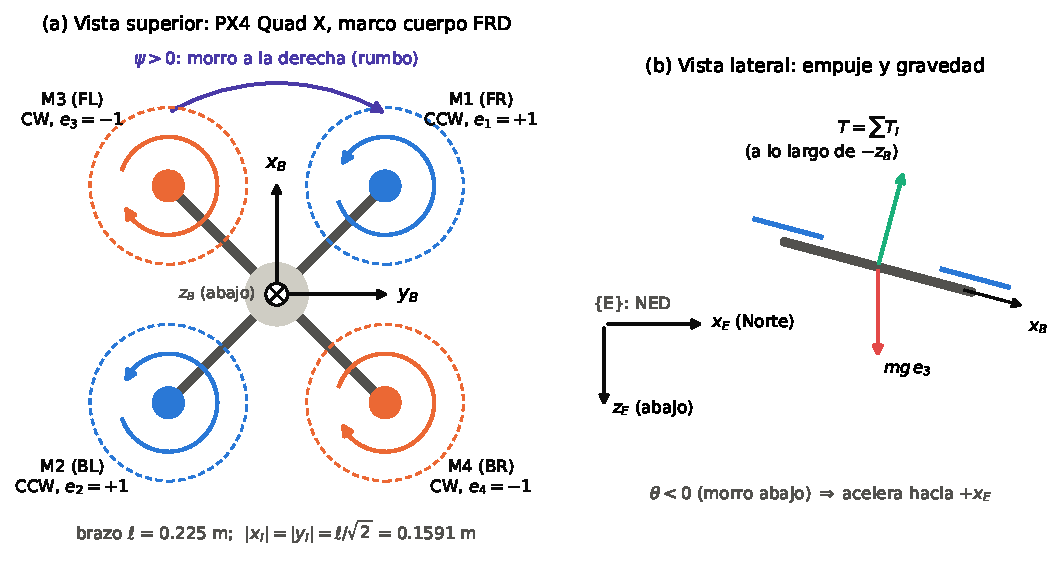
\includegraphics[width=\textwidth]{marco_quad_x.pdf}
\caption{Convenciones. (a) Vista superior del bastidor PX4 Quad X en FRD:
numeración, sentido de giro y signo $e_i$ de cada rotor; el eje $z_B$ entra en
la página. (b) Vista lateral en NED: el empuje actúa a lo largo de $-z_B$; con
el morro abajo ($\theta<0$) su componente horizontal acelera al dron hacia el
norte.}
\label{fig:marco}
\end{figure}

\subsection{Resumen de símbolos}

\begin{table}[H]
\centering
\small
\caption{Notación principal.}
\label{tab:notacion}
\begin{tabularx}{\textwidth}{lX}
\toprule
Símbolo & Significado \\
\midrule
$\vect p,\ \vect v$ & posición y velocidad del centro de masa en $\E$ [m, m/s] \\
$\vect q,\ \R(\vect q)$ & cuaternión de actitud y matriz de rotación $\B\to\E$ \\
$\vect\omega=[p,q,r]\T$ & velocidad angular del cuerpo expresada en $\B$ [rad/s] \\
$\Omega_i$ & velocidad del rotor $i$ [rad/s] \\
$\sigma_i\in[0,1]$ & acelerador enviado al ESC del motor $i$ \\
$C_T,\ C_M$ & coeficientes de empuje y de par: $T_i=C_T\Omega_i^2$, $Q_i=C_M\Omega_i^2$ \\
$C_R,\ \omega_b,\ T_m$ & recta del ESC y constante de tiempo del motor \\
$J=\diag(J_{xx},J_{yy},J_{zz})$ & tensor de inercia en el centro de masa \\
$J_m$ & inercia de rotor + hélice \\
$\vect v_w$ & velocidad del viento en $\E$ \\
$\vect f_B$ & fuerza específica (lo que mide un acelerómetro ideal) \\
$u\in[-1,1]^3$ & momento normalizado que entrega el lazo de tasa \\
\bottomrule
\end{tabularx}
\end{table}

\section{Cinemática}
\label{sec:cinematica}

\subsection{Por qué cuaterniones}

La dinámica se integra con el cuaternión y no con los ángulos de Euler. La
razón es práctica: la cinemática de Euler tiene una singularidad en
$\theta=\pm90^\circ$ (\emph{gimbal lock}), donde la matriz que convierte
velocidad angular en derivadas de los ángulos deja de ser invertible. Un
dron real no vuela de canto, pero un controlador mal sintonizado o una
maniobra acrobática pueden llevarlo ahí, y un simulador que se rompe
justo cuando el controlador falla no sirve para estudiar fallas. El
cuaternión no tiene singularidades, cuesta cuatro números en vez de nueve
(matriz de rotación) y su cinemática es bilineal, lo que facilita la
integración. Los ángulos de Euler se calculan solo para mostrar y para el
lazo de actitud.

\subsection{Ecuaciones}

La cinemática de traslación es la definición de velocidad:
\begin{equation}
\dot{\vect p} = \vect v .
\label{eq:pdot}
\end{equation}
La de rotación, con $\vect\omega$ expresada en el cuerpo
(\cod{math3d.q\_derivative}):
\begin{equation}
\dot{\vect q} = \tfrac12\,\vect q\otimes\begin{bmatrix}0\\ \vect\omega\end{bmatrix}
=\frac12\begin{bmatrix}
-q_x p - q_y q - q_z r\\
\phantom{-}q_w p + q_y r - q_z q\\
\phantom{-}q_w q - q_x r + q_z p\\
\phantom{-}q_w r + q_x q - q_y p
\end{bmatrix},
\label{eq:qdot}
\end{equation}
donde $\otimes$ es el producto de Hamilton. La matriz de rotación asociada
(\cod{math3d.q\_to\_rot}) es
\begin{equation}
\R(\vect q)=\begin{bmatrix}
1-2(q_y^2+q_z^2) & 2(q_xq_y-q_wq_z) & 2(q_xq_z+q_wq_y)\\
2(q_xq_y+q_wq_z) & 1-2(q_x^2+q_z^2) & 2(q_yq_z-q_wq_x)\\
2(q_xq_z-q_wq_y) & 2(q_yq_z+q_wq_x) & 1-2(q_x^2+q_y^2)
\end{bmatrix}.
\label{eq:Rq}
\end{equation}

\paragraph{Conversión con Euler.} De Euler a cuaternión
(\cod{euler\_to\_q}), con $c_\bullet=\cos(\bullet/2)$ y
$s_\bullet=\sin(\bullet/2)$:
\begin{equation}
\vect q=\begin{bmatrix}
c_\phi c_\theta c_\psi + s_\phi s_\theta s_\psi\\
s_\phi c_\theta c_\psi - c_\phi s_\theta s_\psi\\
c_\phi s_\theta c_\psi + s_\phi c_\theta s_\psi\\
c_\phi c_\theta s_\psi - s_\phi s_\theta c_\psi
\end{bmatrix}.
\end{equation}
Y de vuelta (\cod{q\_to\_euler}):
\begin{equation}
\begin{aligned}
\phi&=\operatorname{atan2}\!\big(2(q_wq_x+q_yq_z),\,1-2(q_x^2+q_y^2)\big),\\
\theta&=\arcsin\!\big(\sat_{[-1,1]}\,2(q_wq_y-q_zq_x)\big),\\
\psi&=\operatorname{atan2}\!\big(2(q_wq_z+q_xq_y),\,1-2(q_y^2+q_z^2)\big).
\end{aligned}
\end{equation}
La saturación del argumento del arcoseno evita que el redondeo produzca un
\texttt{NaN} cerca de $\theta=\pm90^\circ$.

\paragraph{Tasas de Euler y velocidad angular.} El lazo de ángulo produce
derivadas deseadas de los ángulos de Euler; el lazo de tasa necesita
velocidades angulares del cuerpo. La relación para Z-Y-X
(\cod{control/attitude.euler\_rates\_to\_body}) es
\begin{equation}
\vect\omega = W(\phi,\theta)\begin{bmatrix}\dot\phi\\ \dot\theta\\ \dot\psi\end{bmatrix},
\qquad
W=\begin{bmatrix}
1 & 0 & -\sin\theta\\
0 & \cos\phi & \sin\phi\cos\theta\\
0 & -\sin\phi & \cos\phi\cos\theta
\end{bmatrix}.
\label{eq:W}
\end{equation}
$W$ deja de ser invertible en $\cos\theta=0$: es la misma singularidad de
Euler, que por eso queda confinada al lazo de ángulo.

\paragraph{Normalización.} La integración numérica de \eqref{eq:qdot} no
conserva exactamente $\|\vect q\|=1$. Después de cada paso de física se
renormaliza (\cod{dynamics.renormalize\_quat}). Es una proyección de orden
del error de truncamiento, que no cambia el orden del método.

\subsection{Verificación}

El bloque B de \cod{model\_verification.py} toma 500 actitudes aleatorias
(roll y pitch hasta $\pm80^\circ$ y $\pm74^\circ$, yaw en $\pm172^\circ$) y
mide el peor caso de cada propiedad:

\begin{table}[H]
\centering
\small
\caption{Verificación numérica de la cinemática (peor caso en 500 actitudes).}
\label{tab:verif_cin}
\begin{tabularx}{\textwidth}{Xr}
\toprule
Propiedad comprobada & Error máximo \\
\midrule
Ortonormalidad, $\max|\R\T\R-I|$ y $|\det\R-1|$ & \val{eOrth} \\
$\R(\vect q)$ de \eqref{eq:Rq} contra $\R_z\R_y\R_x$ de \eqref{eq:zyx} & \val{eZYX} \\
Ida y vuelta Euler $\to\vect q\to$ Euler [rad] & \val{eRound} \\
$W$ de \eqref{eq:W} contra derivadas de Euler obtenidas por diferencias finitas de \eqref{eq:qdot} [rad/s] & \val{eW} \\
Jacobiano analítico $\partial(\R\T\vect d)/\partial\vect q$ usado por Madgwick y el EKF, contra diferencias finitas & \val{eJac} \\
\bottomrule
\end{tabularx}
\end{table}

Los dos primeros errores están en el nivel del redondeo de doble precisión;
los dos últimos son del orden del error de las diferencias finitas usadas
como referencia ($h=10^{-6}$ y $10^{-7}$), no del código.

\section{Dinámica de Newton--Euler completa}
\label{sec:dinamica}

\subsection{Estado y entrada}

El vector de estado tiene 17 componentes (\cod{dynamics.py}, índices
\cod{IP, IV, IQ, IW, IR}):
\begin{equation}
\vect x = \big[\ \vect p\T\ \ \vect v\T\ \ \vect q\T\ \ \vect\omega\T\ \ \Omega_1\ \ \Omega_2\ \ \Omega_3\ \ \Omega_4\ \big]\T\in\mathbb R^{3+3+4+3+4=17} .
\label{eq:estado}
\end{equation}
La entrada son los cuatro aceleradores $\sigma_i\in[0,1]$, retenidos
(orden cero) durante cada paso de integración. Las perturbaciones entran por
un objeto \cod{Environment}: velocidad del viento $\vect v_w$ en $\E$, fuerza
externa $\vect F_{ext}$ en $\E$, momento externo $\vect\tau_{ext}$ en $\B$,
eficiencia de cada motor $\eta_i$ y un indicador de efecto suelo.

Incluir las velocidades de los rotores en el estado, en lugar de suponer que
el empuje sigue instantáneamente al mando, es la diferencia entre un modelo
útil para sintonizar y uno que no lo es. El rezago del motor ($T_m=20$~ms en
el PAE-X450) es el mayor retardo de la cadena de control de actitud; sin él
cualquier ganancia de tasa parece estable.

\subsection{Supuestos}

\begin{supuesto}[Supuestos del modelo de sólido rígido]
\begin{itemize}[leftmargin=1.2em]
\item Tierra plana y no rotante: $\E$ es inercial y la gravedad es uniforme.
A las velocidades y distancias de un multirrotor de laboratorio, la
aceleración de Coriolis terrestre ($\sim10^{-4}$~m/s$^2$) es despreciable.
\item Cuerpo rígido con masa constante (salvo los eventos de carga útil,
\cref{sec:perturbaciones}) y tensor de inercia diagonal (productos de inercia
nulos por simetría).
\item Rotores en el plano horizontal que contiene al centro de masa: el
empuje no genera momento por un brazo vertical.
\item Las fuerzas aerodinámicas del fuselaje actúan en el centro de masa.
\end{itemize}
\end{supuesto}

\subsection{Traslación (Newton, en el marco inercial)}

\begin{equation}
m\,\dot{\vect v} = m g\,\eu + \R(\vect q)\,\vect f_B + \vect F_{ext},
\qquad
\vect f_B = \begin{bmatrix} f_{a,x}\\ f_{a,y}\\ f_{a,z} - \sum_{i=1}^4 T_i\end{bmatrix},
\label{eq:newton}
\end{equation}
con $T_i = C_T\Omega_i^2$ (multiplicado por el factor de efecto suelo cuando
está activo) y $\vect f_a$ la fuerza aerodinámica del fuselaje en $\B$
(\cref{sec:aero}). La ecuación se escribe en $\E$ porque ahí la gravedad es
constante y la posición se integra directamente; la fuerza de los rotores
se escribe en $\B$ porque ahí es constante en dirección. La matriz $\R$ hace
el puente, y con ella entra el acoplamiento que la 2.ª edición no tenía:
inclinar el dron inclina el empuje, y el dron se desplaza.

\subsection{Rotación (Euler, en el marco cuerpo)}

El momento angular total del vehículo es el del cuerpo más el de los cuatro
rotores. Si cada rotor gira con velocidad $\Omega_i$ alrededor de $z_B$ en el
sentido $e_i$, un rotor antihorario visto desde arriba tiene su vector de
velocidad angular hacia arriba, es decir, hacia $-z_B$. El momento angular
de los rotores es entonces
\begin{equation}
\vect h_r = \begin{bmatrix}0\\0\\h_z\end{bmatrix},\qquad
h_z = -J_m\sum_{i=1}^4 e_i\,\Omega_i .
\label{eq:hr}
\end{equation}
Derivando $J\vect\omega+\vect h_r$ en el marco móvil e igualando al momento
externo se obtiene
\begin{equation}
J\dot{\vect\omega} = \vect\tau_B - \vect\omega\times(J\vect\omega)
 - \vect\omega\times\vect h_r - \underset{\scriptscriptstyle \text{omitido}}{\dot{\vect h}_r}
 + \vect\tau_a + \vect\tau_{ext},
\label{eq:euler}
\end{equation}
donde el momento de los rotores es
\begin{equation}
\vect\tau_B=\begin{bmatrix}\tau_x\\ \tau_y\\ \tau_z\end{bmatrix}
=\begin{bmatrix}
-\sum_i y_i\,T_i\\
\phantom{-}\sum_i x_i\,T_i\\
\phantom{-}\sum_i e_i\,Q_i
\end{bmatrix},\qquad Q_i=C_M\Omega_i^2 .
\label{eq:tauB}
\end{equation}
El signo de la fila de roll sale del producto cruz: el rotor $i$ está en
$(x_i,y_i,0)$ y empuja con $(0,0,-T_i)$, así que
$(x_i,y_i,0)\times(0,0,-T_i)=(-y_iT_i,\ x_iT_i,\ 0)$. Un rotor a la derecha
($y_i>0$) que empuja más produce roll negativo (levanta el ala derecha).

En componentes, con $J$ diagonal, el código (\cod{QuadrotorDynamics.derivative})
evalúa
\begin{align}
J_{xx}\dot p &= \tau_x - (J_{zz}-J_{yy})\,q r - q\,h_z + \tau_{a,x} + \tau_{ext,x},\nonumber\\
J_{yy}\dot q &= \tau_y - (J_{xx}-J_{zz})\,r p + p\,h_z + \tau_{a,y} + \tau_{ext,y},\label{eq:euler_comp}\\
J_{zz}\dot r &= \tau_z - (J_{yy}-J_{xx})\,p q + \tau_{a,z} + \tau_{ext,z}.\nonumber
\end{align}

\paragraph{El término giroscópico de los rotores, $-\vect\omega\times\vect h_r$.}
Solo afecta a roll y pitch, y es proporcional a la \emph{diferencia} entre
las velocidades de los rotores CCW y CW. En hover esa diferencia es cero y el
término desaparece; aparece cuando hay mando de guiñada mientras el dron
gira en roll o pitch. Con $J_m/J_{zz}=\val{JmJz}$ su efecto es pequeño en el
PAE-X450, pero se incluye porque no cuesta nada y está en todos los modelos
de referencia \cite{qq17,hb11}.

\subsection{El término de reacción por aceleración de los rotores, omitido}
\label{sec:reaccion}

El término $-\dot{\vect h}_r = J_m\sum_i e_i\dot\Omega_i\,\vect e_3$ es la
reacción que siente el cuerpo cuando los motores \emph{aceleran} sus rotores.
Está en las ecuaciones de Phang et al.\ \cite{hb11} (ecs.~11.14--11.16), y el
código lo calcula, pero no lo aplica, salvo que la dinámica se construya
con la opción \cod{include\_rotor\_reaction=True}. La decisión no es
de comodidad; es de consistencia con el resto del modelo.

Con el propulsor de primer orden de la \cref{sec:propulsion}, un escalón del
acelerador desde hover hasta el máximo produce, en el primer instante,
\begin{equation}
\dot\Omega = \frac{\Omega_{max}-\Omega_h}{T_m}
= \frac{\val{wmax}-\val{wh}}{0.02} = \val{dOm}\ \text{rad/s}^2,
\qquad
J_m\dot\Omega = \val{reac}\ \text{N·m por motor}.
\end{equation}
Ese par tendría que darlo el motor. Un motor 2212 de 920~KV (el típico de un
F450) tiene $K_t = 60/(2\pi\cdot920) = \val{Kt}$~N·m/A; con un límite de
corriente de 15~A (supuesto razonable para un ESC de 20--30~A) entrega como
mucho $\val{taumot}$~N·m, unas \val{reacRatio} veces menos. El par
aerodinámico máximo de la hélice es $\val{Qmax}$~N·m, \val{reacRatioAero}
veces menor que esa reacción. En un motor real la corriente se satura y la
aceleración del rotor queda limitada por el par disponible; el modelo de
primer orden no tiene esa saturación, de modo que su $\dot\Omega$ inicial es
físicamente inalcanzable.

Aplicar $\dot{\vect h}_r$ con ese $\dot\Omega$ generaría golpes de guiñada
de casi 3~N·m (ocho veces el momento máximo de guiñada del vehículo,
$\val{taumaxY}$~N·m) que el dron real no siente. Modelarlo bien exige un
modelo eléctrico del motor con límite de corriente, que queda como trabajo
futuro (\cref{sec:limitaciones}). El modelo de Quan \cite{qq17} (cap.~6) y
su implementación CopterSim \cite{cs19}, de donde provienen los parámetros
del PAE-X450, tampoco incluyen este término: la omisión es coherente con la
fuente de los datos.

\subsection{Dinámica de los rotores}

Cada rotor sigue un primer orden hacia la velocidad de régimen que impone su
ESC (\cref{sec:propulsion}):
\begin{equation}
T_m\,\dot\Omega_i = \eta_i\,\omega_{ss}(\sigma_i) - \Omega_i ,
\label{eq:rotor}
\end{equation}
con $\eta_i\in(0,1]$ la eficiencia del motor (1 salvo en el escenario de falla,
\cref{sec:perturbaciones}).

\subsection{Fuerza específica y contacto con el suelo}

El acelerómetro ideal mide la fuerza específica, que el código calcula a
partir de la derivada del estado (\cod{specific\_force\_B}):
\begin{equation}
\vect f_{acc} = \R\T\big(\dot{\vect v} - g\,\eu\big)
= \frac{1}{m}\Big(\vect f_B + \R\T\vect F_{ext}\Big).
\label{eq:fesp}
\end{equation}
La segunda igualdad, que sale de \eqref{eq:newton}, tiene una consecuencia
que reaparece en la \cref{sec:estimadores}: el acelerómetro de un
multirrotor mide empuje y arrastre, nunca la gravedad. En hover inclinado y
sin velocidad mide $(0,0,-g)$ \emph{independientemente} de la inclinación.

El suelo se trata como una restricción unilateral simple
(\cod{Simulation.\_ground\_contact}): si $z>0$ se fija $z=0$ y se anula la
velocidad vertical descendente; si además el empuje total es menor que el
peso, el dron queda apoyado en sus patas: velocidad horizontal y angular
nulas y actitud nivelada conservando el rumbo. No hay fricción ni rebote:
basta para despegar y aterrizar, no para estudiar aterrizajes.

\section{Propulsor y asignación de control}
\label{sec:propulsion}

\subsection{Modelo ESC + motor sin escobillas + hélice}

El controlador de vuelo no manda empuje: manda un acelerador $\sigma$
(un ancho de pulso o un valor DShot normalizado) a un ESC, y el ESC lleva el
motor a una velocidad. El modelo de \cod{propulsion.py} sigue la cadena
física en ese orden, con las ecuaciones del cap.~4 de Quan \cite{qq17} y de
CopterSim \cite{cs19}:
\begin{align}
\omega_{ss}(\sigma) &= \begin{cases}
0 & \sigma < \sigma_{dz}\\
\max\!\big(0,\ C_R\,\sigma + \omega_b\big) & \sigma\ge\sigma_{dz}
\end{cases}
&&\text{(velocidad de régimen del ESC)}\label{eq:esc}\\
T_m\,\dot\Omega &= \omega_{ss} - \Omega &&\text{(dinámica del rotor)}\label{eq:motor}\\
T &= C_T\,\Omega^2,\qquad Q = C_M\,\Omega^2 &&\text{(empuje y par de arrastre)}\label{eq:TQ}
\end{align}

La recta \eqref{eq:esc} es lo que se mide en un banco poniendo escalones de
acelerador y registrando las rpm en régimen; $T_m$ sale de la respuesta al
escalón. Es la misma estructura que Powers, Mellinger y Kumar \cite{hb16}
(p.~312) escriben como $\dot\omega = k_m(\omega^{des}-\omega)$, con la recta
del ESC delante. Para el PAE-X450, $C_R=1148$~rad/s, $\omega_b=-141.4$~rad/s,
$T_m=0.02$~s y $\sigma_{dz}=0.05$.

\begin{nota}[La zona muerta en el PAE-X450]
Con $\omega_b<0$ la recta cruza cero en $\sigma_0=-\omega_b/C_R=0.123$. Por
debajo de ese acelerador el ESC ya entrega velocidad nula por el
$\max(0,\cdot)$, de modo que la zona muerta explícita $\sigma_{dz}=0.05$ no
cambia nada en este vehículo: la zona muerta efectiva es $[0,\,0.123)$. El
parámetro existe para los vehículos del catálogo cuyo ESC se modela sin
desplazamiento.
\end{nota}

\paragraph{¿Por qué cuadrático?} Para una hélice de paso fijo en aire
quieto, la teoría de cantidad de movimiento y los ensayos estáticos dan
$T\propto\Omega^2$ y $Q\propto\Omega^2$ con buena aproximación. Quitian Niño
\cite{quitian22}, midiendo rotores en banco en esta misma universidad,
encontró que un ajuste $T=b\Omega^2+a\Omega+c$ es estadísticamente mejor;
el simulador conserva la forma cuadrática pura porque hace lineal la
asignación de control en $s_i=\Omega_i^2$ y porque es la forma que usan los
datos de la fuente. Si al comparar con un banco real apareciera un sesgo
sistemático a bajas revoluciones, este es el primer sospechoso.

\subsection{Matriz de asignación}

Empuje colectivo y momentos son lineales en $s_i=\Omega_i^2$
(\cref{eq:tauB}):
\begin{equation}
\begin{bmatrix}T\\ \tau_x\\ \tau_y\\ \tau_z\end{bmatrix}
= \underset{\scriptscriptstyle B}{\begin{bmatrix}
C_T & C_T & C_T & C_T\\
-y_1C_T & -y_2C_T & -y_3C_T & -y_4C_T\\
x_1C_T & x_2C_T & x_3C_T & x_4C_T\\
e_1C_M & e_2C_M & e_3C_M & e_4C_M
\end{bmatrix}}
\begin{bmatrix}s_1\\ s_2\\ s_3\\ s_4\end{bmatrix}.
\label{eq:B}
\end{equation}
Con los rotores de la \cref{tab:rotores} y $aC_T=1.758\times10^{-6}$:
\begin{equation}
B_{\text{PAE-X450}}=\begin{bmatrix}
1.105 & 1.105 & 1.105 & 1.105\\
-0.1758 & 0.1758 & 0.1758 & -0.1758\\
0.1758 & -0.1758 & 0.1758 & -0.1758\\
0.01779 & 0.01779 & -0.01779 & -0.01779
\end{bmatrix}\times10^{-5}.
\end{equation}
Su número de condición es \val{condB} y $\max|BB^{-1}-I|=\val{eBinv}$. La
matriz se invierte una vez al construir el mezclador (\cod{Mixer.\_\_init\_\_});
en el lazo solo se multiplican columnas de $B^{-1}$. El paso inverso de
$s_i$ a acelerador usa la recta del ESC en régimen,
\begin{equation}
\sigma_i=\sat_{[0,1]}\!\left(\frac{\sqrt{s_i}-\omega_b}{C_R}\right)
\quad(\sigma_i=0 \text{ si } s_i\approx0),
\label{eq:escinv}
\end{equation}
igual que un autopiloto real, que tampoco conoce la velocidad instantánea
de los rotores.

\paragraph{Comprobación de signos.} Pidiendo el empuje de hover más un
momento de $+0.2$~N·m en cada eje (\cref{tab:signos}), los motores que suben
son los que deben subir, y el momento que resulta al pasar las velocidades
de régimen por $B$ es exactamente el pedido.

\begin{table}[H]
\centering
\small
\caption{Aceleradores (M1, M2, M3, M4) para $T=mg$ y un momento positivo en
un eje. El momento recuperado con $B$ coincide con el pedido a 4 cifras.}
\label{tab:signos}
\begin{tabular}{lll}
\toprule
Momento pedido & $\sigma$ (M1 FR, M2 BL, M3 FL, M4 BR) & Lectura \\
\midrule
$\tau_x=+0.2$~N·m & \val{sigroll} & suben los izquierdos: ala derecha abajo \\
$\tau_y=+0.2$~N·m & \val{sigpitch} & suben los delanteros: morro arriba \\
$\tau_z=+0.05$~N·m & \val{sigyaw} & suben los CCW: morro a la derecha \\
\bottomrule
\end{tabular}
\end{table}

\subsection{Desaturación por prioridades}

Cuando la combinación pedida no cabe en $s_i\in[0,\Omega_{max}^2]$, algo hay
que sacrificar. El mezclador (\cod{Mixer.allocate}) lo hace con la misma
prioridad que PX4: primero se protege la actitud en roll y pitch (lo que
mantiene al dron derecho), después el empuje y al final la guiñada, que es
el eje menos crítico y el más débil. Separando
$\vect s=\vect s_T+\vect s_{RP}+\vect s_Y$ en las contribuciones de cada
columna de $B^{-1}$:

\begin{enumerate}
\item Si el rango de $\vect s_{RP}$ (máximo menos mínimo) excede
$\Omega_{max}^2$, ni con el colectivo ideal cabe: se escala
$\vect s_{RP}\leftarrow k_{rp}\vect s_{RP}$, $k_{rp}=\Omega_{max}^2/\text{rango}$.
\item Se desplaza el colectivo con un mismo $\Delta s$ en los cuatro motores
para que $\vect s_T+k_{rp}\vect s_{RP}$ quede dentro de $[0,\Omega^2_{max}]$.
Esto sacrifica empuje, no actitud.
\item Se agrega la guiñada con el mayor $k_y\in[0,1]$ que no saque a ningún
motor del intervalo.
\end{enumerate}

Dos casos de la verificación (bloque C) lo muestran. Con empuje del 90~\%
del máximo, $\tau_x=3$~N·m y $\tau_z=0.3$~N·m, el resultado es
$\sigma=(\val{desatSig})$: el roll se cumple completo
($\tau_x=\val{desatTx}$~N·m), el colectivo baja \val{desatShift}~N (de 40.3 a
\val{desatT}~N) y la guiñada se anula ($k_y=\val{desatKy}$). En el extremo
opuesto, con empuje del 30~\% del peso y $\tau_x=1$~N·m, el mezclador
\emph{sube} el colectivo $\val{lowShift}$~N para poder crear el momento,
$\sigma=(\val{lowSig})$. Ese segundo caso es la razón física por la que un
multirrotor pierde autoridad de actitud en descensos rápidos con los motores
cerca del ralentí: no hay colectivo del cual restar. Los factores $k_{rp}$,
$k_y$ y el desplazamiento de empuje se publican en la telemetría.

\subsection{Momentos máximos}

El lazo de tasa entrega un momento normalizado $u\in[-1,1]$ por eje, que se
convierte en N·m multiplicando por el momento máximo del eje
(\cod{VehicleParams.max\_torque}): los rotores que empujan a favor a fondo y
los que empujan en contra en cero,
\begin{equation}
\tau_{x,max}=\sum_{y_i<0}|y_i|\,C_T\Omega_{max}^2=\val{taumaxR}~\text{N·m},\qquad
\tau_{z,max}=\sum_{e_i>0}C_M\Omega_{max}^2=\val{taumaxY}~\text{N·m}.
\label{eq:taumax}
\end{equation}
La guiñada tiene \val{tauRY} veces menos autoridad que el roll. No se fijó a
mano: sale del cociente $C_M/(aC_T)$, y explica por qué en cualquier
multirrotor el yaw es el eje lento.

\section{Aerodinámica del fuselaje, viento y efecto suelo}
\label{sec:aero}

\subsection{Arrastre de traslación}

El modelo de arrastre es el de CopterSim \cite{cs19} (ec.~1.19 de
\cite{qq20}): cuadrático en la velocidad \emph{relativa al aire}, por eje del
cuerpo, más un término lineal opcional que usan los vehículos tomados de
Luukkonen \cite{luukkonen11}:
\begin{gather}
\vect v_{r,B} = \R\T\big(\vect v - \vect v_w\big),\label{eq:vrel}\\
f_{a,j} = -C_{d,xy}\,v_{r,j}|v_{r,j}| - A\,v_{r,j}\quad (j=x,y),\qquad
f_{a,z} = -C_{d,z}\,v_{r,z}|v_{r,z}| - A\,v_{r,z}.\label{eq:drag}
\end{gather}
Para el PAE-X450, $C_{d,xy}=0.055$~N/(m/s)$^2$ y $A=0$.

El viento entra únicamente aquí, como velocidad del aire. Esa es la forma
físicamente correcta: el viento no ``empuja'' al dron con una fuerza
externa arbitraria, sino que cambia la velocidad relativa sobre la que actúa
el arrastre. Dos consecuencias se ven en el simulador sin programarlas: un
dron quieto en un viento de 3~m/s del norte siente
$0.055\cdot3^2\approx0.50$~N hacia el sur y tiene que inclinarse unos
$\arctan(0.50/13.7)\approx2^\circ$ contra el viento para mantener su
posición; y un dron que vuela con el viento a favor a la velocidad del
viento no siente arrastre alguno.

\begin{supuesto}[Arrastre vertical]
CopterSim solo modela arrastre en $x_B,y_B$. El simulador agrega
$C_{d,z}=C_{d,xy}$ como supuesto (campo \cod{caveats} del vehículo). En
ascensos y descensos lentos su efecto es pequeño; no debe usarse para
estudiar descensos rápidos dentro de la propia estela (anillo de vórtices),
que este modelo no representa.
\end{supuesto}

\subsection{Amortiguamiento rotacional}

\begin{equation}
\vect\tau_a = -\begin{bmatrix}
C_{Cm,x}\,p|p|\\ C_{Cm,y}\,q|q|\\ C_{Cm,z}\,r|r|
\end{bmatrix},
\qquad C_{Cm}=(0.0035,\ 0.0039,\ 0.0034)\ \text{N·m/(rad/s)}^2 .
\label{eq:damp}
\end{equation}
Los coeficientes son los de CopterSim. A 3~rad/s el amortiguamiento de roll
vale unos 0.03~N·m, menos del 1~\% de $\tau_{x,max}$: no cambia la
naturaleza integradora del lazo de tasa, pero acota la velocidad angular
en lazo abierto. La 2.ª edición dejaba este término en cero por falta de
fuente; ahora la tiene.

\subsection{Efecto suelo}

Cerca del suelo la estela del rotor se frena contra la superficie y el rotor
produce más empuje con la misma potencia. Con el modelo clásico de
Cheeseman y Bennett \cite{cheeseman55}, a una altura $h$ y para un rotor de
radio $R_p$,
\begin{equation}
k_{ge}(h) = \frac{T_{IGE}}{T_{OGE}} = \frac{1}{1-\left(\dfrac{R_p}{4h}\right)^2},
\qquad k_{ge}\le1.4,
\label{eq:ge}
\end{equation}
y se aplica como factor sobre cada $T_i$ (\cod{dynamics.py}). El tope de
1.4 (también para $h\le2$~cm) evita la singularidad en $h=R_p/4$, donde la
fórmula deja de ser válida. Con $R_p=0.12$~m:

\begin{table}[H]
\centering
\small
\caption{Factor de efecto suelo para $R_p=0.12$~m.}
\label{tab:ge}
\begin{tabular}{lccccc}
\toprule
$h$ [m] & 0.06 & 0.12 & 0.24 & 0.5 & 1.0 \\
$k_{ge}$ & \val{gea} & \val{geb} & \val{gec} & \val{ged} & \val{gee} \\
\bottomrule
\end{tabular}
\end{table}

A partir de una altura de dos diámetros el efecto es menor del 0.4~\%. Está
apagado por defecto y se activa en \cod{DisturbanceConfig(ground\_effect=True)};
es útil para estudiar despegues y aterrizajes, no para el vuelo de
seguimiento que se evalúa en este trabajo.

\section{Parámetros del vehículo de referencia y del catálogo}
\label{sec:parametros}

\subsection{Por qué el PAE-X450}

Un modelo con ecuaciones correctas y parámetros inventados no sirve para
sintonizar nada. La 2.ª edición armaba su vehículo con números de distintas
tesis, y la \cref{sec:proposito} mostró que ni siquiera dentro de una misma
tesis eran coherentes. La 3.ª edición adopta como vehículo por defecto un
cuadricóptero en X de clase 450~mm y 1.4~kg (motores sin escobillas, ESC y
hélices de unos 10~pulgadas: el ``dron mediano normal'' de laboratorio) cuyos
parámetros vienen \emph{todos} de una misma fuente: el modelo por defecto de
CopterSim, el simulador del grupo de Quan Quan en la Universidad de Beihang,
base de la plataforma RflySim y de los libros \cite{qq17,qq20}.

La fuente primaria es el archivo de inicialización del modelo Simulink,
\cod{Init.m}, del repositorio \cod{github.com/XunhuaDai/CopterSim}, commit
\cod{0d14487f} (25 de julio de 2019) \cite{cs19}, en el que cada parámetro
viene comentado. Los valores de la \cref{tab:pae} se cotejaron contra ese
archivo el 4 de octubre de 2026 y coinciden dígito a dígito.

\begin{table}[H]
\centering
\small
\caption{Parámetros del PAE-X450 (\cod{vehicles.PAE\_X450}). Fuente: \cod{Init.m}
de CopterSim \cite{cs19}, modelo por defecto de \cite{qq20,qq17}, salvo donde
se indica.}
\label{tab:pae}
\setlength{\tabcolsep}{4pt}
\begin{tabularx}{\textwidth}{>{\raggedright\arraybackslash}p{3.9cm}l>{\raggedright\arraybackslash}p{2.6cm}l>{\raggedright\arraybackslash}X}
\toprule
Parámetro & Símbolo & Valor & Unidad & Nombre en \cod{Init.m} / nota \\
\midrule
Masa & $m$ & 1.4 & kg & \cod{uavMass} \\
Brazo (centro a eje del motor) & $\ell$ & 0.225 & m & \cod{uavR} \\
Inercias & $J_{xx},J_{yy},J_{zz}$ & 0.0241, 0.0239, 0.0386 & kg·m$^2$ & \cod{uavJxx/yy/zz}; productos de inercia nulos \\
Coeficiente de empuje & $C_T$ & $1.105\times10^{-5}$ & N/(rad/s)$^2$ & \cod{rotorCt} \\
Coeficiente de par & $C_M$ & $1.779\times10^{-7}$ & N·m/(rad/s)$^2$ & \cod{rotorCm} \\
Inercia rotor + hélice & $J_m$ & $1.287\times10^{-4}$ & kg·m$^2$ & \cod{motorJm} \\
Pendiente del ESC & $C_R$ & 1148 & rad/s & \cod{motorCr} \\
Ordenada del ESC & $\omega_b$ & $-141.4$ & rad/s & \cod{motorWb} \\
Constante de tiempo del motor & $T_m$ & 0.02 & s & \cod{motorT} \\
Zona muerta del acelerador & $\sigma_{dz}$ & 0.05 & --- & \cod{motorMinThr} \\
Arrastre horizontal & $C_{d,xy}$ & 0.055 & N/(m/s)$^2$ & \cod{uavCd} \\
Arrastre vertical & $C_{d,z}$ & 0.055 & N/(m/s)$^2$ & \textbf{supuesto}: igual a $C_{d,xy}$ \\
Amortiguamiento rotacional & $C_{Cm}$ & 0.0035, 0.0039, 0.0034 & N·m/(rad/s)$^2$ & \cod{uavCCm} \\
Acelerador de hover declarado & --- & 0.609 & --- & \cod{BattHoverThr}; solo para comprobar \\
\bottomrule
\end{tabularx}
\end{table}

\begin{supuesto}[Lo que no viene de CopterSim]
El arrastre vertical; el voltaje constante (CopterSim trae un modelo de
batería que aquí no se implementa); y el punto de aplicación del arrastre:
\cod{Init.m} declara una distancia vertical de 0.12~m entre el centro
aerodinámico y el centro de masa (\cod{uavDearo}), que produciría un momento
de cabeceo proporcional al arrastre. El simulador aplica el arrastre en el
centro de masa y no modela ese momento (\cref{sec:limitaciones}).
\end{supuesto}

\subsection{Chequeos de consistencia}

Un conjunto de parámetros tomado de una fuente puede tener erratas. La
forma de detectarlas es cruzar cantidades que la fuente da por separado y
que la física obliga a que coincidan. El bloque A de
\cod{model\_verification.py} hace cinco cruces.

\paragraph{Velocidad y acelerador de hover.} El rotor sostiene el hover
cuando $4C_T\Omega_h^2=mg$:
\begin{equation}
\Omega_h=\sqrt{\frac{mg}{4C_T}}=\val{wh}~\text{rad/s}\ (\val{whrpm}~\text{rpm}),\qquad
\sigma_h=\frac{\Omega_h-\omega_b}{C_R}=\val{sigmah}.
\label{eq:hover}
\end{equation}
\cod{Init.m} declara por separado un acelerador de hover de
\val{sigmahd}. Que el valor calculado desde masa, $C_T$ y la recta del ESC
coincida con el declarado a la tercera cifra indica que propulsor y masa son
coherentes entre sí: es exactamente la prueba que el F450 de Jiřinec no pasa.

\paragraph{Coeficiente de empuje adimensional.} La literatura de hélices
reporta el coeficiente estático $C_T'=T/(\rho n^2D^4)$, con $n$ en rev/s. Con
$\Omega=2\pi n$, $C_T'=4\pi^2C_T/(\rho D^4)$. Suponiendo la hélice de
9.4~pulgadas (0.239~m) que monta un F450 (supuesto: \cod{Init.m} no declara
el diámetro) y $\rho=1.225$~kg/m$^3$, resulta $C_T'=\val{CTad}$ y
$C_P'=2\pi C_Q'=\val{CPad}$. Son valores del orden de los que publican las
bases de ensayos estáticos para hélices de dos palas de ese tamaño (UIUC
Propeller Data Site \cite{uiuc}), lo que descarta un error de unidades en
$C_T$ y $C_M$, por ejemplo una confusión entre rpm y rad/s, que cambiaría el
coeficiente en un factor $(60/2\pi)^2\approx91$.

\paragraph{Relación par/empuje.} $C_M/C_T=\val{CmCt}$~m, típica de
hélices de 9--10~pulgadas; de ella sale la autoridad de guiñada.

\paragraph{Empuje máximo.} Con $\sigma=1$, $\Omega_{max}=C_R+\omega_b=\val{wmax}$~rad/s
(\val{wmaxrpm}~rpm) y cada rotor da $C_T\Omega_{max}^2=\val{Tmax}$~N
(\val{Tmaxkgf}~kgf). La relación empuje/peso es $\val{TW}$, normal para un
F450 con batería 4S y suficiente para maniobrar con margen.

\paragraph{Frecuencia de paso de pala.} Con dos palas, la vibración por
desbalance aparece a $f_{bp}=2\Omega/(2\pi)$: \val{fbp}~Hz en hover y
\val{fbpmax}~Hz a acelerador máximo. Este número gobierna el diseño de los
filtros (\cref{sec:sensores,sec:filtros}).

\subsection{Otros vehículos del catálogo}

El catálogo (\cod{VEHICLES}) conserva cuatro vehículos más, útiles para
mostrar que el método de sintonía se adapta solo cuando cambia la física. La
\cref{tab:catalogo} resume sus parámetros y las cantidades derivadas
calculadas por el mismo código.

\begin{table}[H]
\centering
\small
\setlength{\tabcolsep}{5pt}
\caption{Catálogo de vehículos (valores y derivados calculados por \cod{vehicles.py}).}
\label{tab:catalogo}
\begin{tabular}{lccccc}
\toprule
 & \val{catHead} \\
\midrule
\val{catT}
\bottomrule
\end{tabular}
\end{table}

Las fuentes y advertencias de cada uno están en sus campos \cod{source} y
\cod{caveats}:
\begin{itemize}
\item \textbf{Jiřinec (+)} \cite{jirinec11}: inercias (ec.~4.7), $b$ (ec.~4.9),
$d$ (p.~28), motor $0.7/(0.1s+1)$ (ec.~4.6), brazo 0.214~m. Corregido a
1.321~kg y bastidor + (\cref{sec:proposito}). ESC lineal sin
desplazamiento y empuje/peso 3.0 son supuestos; el arrastre lineal
0.25~kg/s viene de Luukkonen.
\item \textbf{Luukkonen} \cite{luukkonen11} (tabla~1, que toma los valores de
Tayebi y McGilvray): rotores instantáneos en la fuente, por lo que
$T_m=0.05$~s es supuesto.
\item \textbf{NUS KayLion} \cite{hb11}: el único con todo medido en banco
(ecs.~11.18--11.27), incluida $T_m=0.0821$~s. Empuje/peso 2.0 deducido de
su banco.
\item \textbf{AscTec Hummingbird} \cite{hb16} (tablas~16.1--16.2): sus
coeficientes venían en N/rpm$^2$; convertidos dividiendo por
$(2\pi/60)^2$ dan $k_F=\val{hbkF}$ y $k_M=\val{hbkM}$ en unidades SI.
\end{itemize}
En los cuatro, el ESC se modela como recta sin desplazamiento
($\omega_b=0$) con $C_R$ elegido para la relación empuje/peso indicada, lo
que fija $\sigma_h=1/\sqrt{T/W}$. Para estos vehículos el acelerador de
hover es una consecuencia de ese supuesto, no un dato.

\section{Linealización en hover y evidencia de que el modelo no lineal la recupera}
\label{sec:linealizacion}

La linealización en vuelo estacionario no se usa para simular: el
simulador integra siempre el modelo completo. Se usa para dos cosas. Para
\emph{diseñar} controladores (las reglas SIMC de la \cref{sec:control} y el
MPC lineal de la \cref{sec:posicion} parten de ella), y para \emph{verificar}
el código: si el modelo no lineal está bien programado, su jacobiano numérico
en hover tiene que coincidir con las derivadas analíticas, y su respuesta a
ángulos pequeños tiene que coincidir con la del modelo lineal.

\subsection{Punto de equilibrio}

Con $\vect v=\vect0$, $\vect q=(1,0,0,0)$, $\vect\omega=\vect 0$,
$\Omega_i=\Omega_h$ y $\sigma_i=\sigma_h$ de \eqref{eq:hover}, todas las
derivadas de \eqref{eq:newton}--\eqref{eq:rotor} se anulan. El residuo
numérico de \cod{derivative} en ese punto es $\max|\dot{\vect x}|=\val{resHover}$,
y diez segundos de integración RK4 en lazo abierto desde el equilibrio
terminan con una velocidad de $\val{driftV}$~m/s: el equilibrio es exacto
hasta el redondeo. El acelerómetro ideal mide en ese estado $(0,0,-g)$.

\subsection{Modelo linealizado}

Con ángulos pequeños, $\vect q\approx(1,\phi/2,\theta/2,\psi/2)$ y
$\R\approx I+\sk{(\phi,\theta,\psi)}$. Escribiendo
$\delta\Omega_i=\Omega_i-\Omega_h$ y $\delta\sigma_i=\sigma_i-\sigma_h$:
\begin{align}
\dot v_x &= -g\,\theta, \qquad \dot v_y = g\,\phi, \qquad
\dot v_z = -\frac{2C_T\Omega_h}{m}\sum_i\delta\Omega_i, \label{eq:lin_tras}\\
\dot\phi &= p,\qquad \dot\theta=q,\qquad \dot\psi=r, \label{eq:lin_cin}\\
\dot p &= \frac{2C_T\Omega_h}{J_{xx}}\sum_i(-y_i)\,\delta\Omega_i,\quad
\dot q = \frac{2C_T\Omega_h}{J_{yy}}\sum_i x_i\,\delta\Omega_i,\quad
\dot r = \frac{2C_M\Omega_h}{J_{zz}}\sum_i e_i\,\delta\Omega_i, \label{eq:lin_rot}\\
T_m\,\delta\dot\Omega_i &= C_R\,\delta\sigma_i - \delta\Omega_i. \label{eq:lin_mot}
\end{align}
Desaparecen tres familias de términos. $\vect\omega\times J\vect\omega$ y el
amortiguamiento $C_{Cm}\omega|\omega|$ son de segundo orden en $\vect\omega$;
el término giroscópico se anula porque en hover $h_z=0$ (dos rotores giran
en cada sentido a la misma velocidad); el arrastre cuadrático tiene
derivada nula en $\vect v=\vect0$. Lo que queda es la estructura que justifica
la cascada de control: cada eje angular es un doble integrador detrás de un
primer orden (el motor), y la traslación horizontal es otro doble integrador
cuya entrada es el ángulo. Powers, Mellinger y Kumar \cite{hb16} (pp.~318--319)
lo dicen en una frase: en ángulos pequeños las aceleraciones angulares
están desacopladas, cada una depende solo de su componente de momento.

\subsection{Jacobiano numérico contra derivadas analíticas}

El bloque D calcula por diferencias centrales el jacobiano $\partial\dot{\vect x}/\partial\vect x$
del modelo completo en hover y lo compara con \eqref{eq:lin_tras}--\eqref{eq:lin_rot}:

\begin{table}[H]
\centering
\small
\caption{Jacobiano del modelo no lineal en hover frente a la linealización analítica.}
\label{tab:jac}
\begin{tabular}{lll}
\toprule
Derivada & Numérica (modelo completo) & Analítica \\
\midrule
$\partial\dot v_y/\partial\phi$, $\partial\dot v_x/\partial\theta$ & $9.80665$, $-9.80665$ & $g$, $-g$ \\
$\partial\dot v_z/\partial\Omega_i$ [m/s$^2$ por rad/s] & \val{dvzdO} & $-2C_T\Omega_h/m$, idéntico a 10 cifras \\
$\partial\dot p/\partial\Omega_i$ (M1, M2, M3, M4) & $\mp\val{dpdO}$ con signos $(-,+,+,-)$ & $-y_i\,2C_T\Omega_h/J_{xx}$ \\
$\partial\dot r/\partial\Omega_i$ & $\pm\val{drdO}$ con signos $(+,+,-,-)$ & $e_i\,2C_M\Omega_h/J_{zz}$ \\
$\max|\partial\dot{\vect\omega}/\partial\vect\omega|$ & \val{cross} & 0 \\
Autovalores & 13 nulos y cuatro en \val{eigMin} & 0 y $-1/T_m=-50$ \\
\bottomrule
\end{tabular}
\end{table}

\subsection{Ganancia de planta del lazo de tasa}

Para el diseño del lazo de tasa interesa la ganancia entre el momento
normalizado $u$ y la aceleración angular. De \eqref{eq:lin_rot} y del
mezclador, en régimen,
\begin{equation}
\frac{\dot p}{u} = K_x = \frac{\tau_{x,max}}{J_{xx}} = \val{Kpred}~\text{rad/s}^2 .
\label{eq:Krate}
\end{equation}
Aplicando un escalón $u=0.02$ al modelo completo a través del mezclador real,
la ganancia medida es \val{Kmed1} a los 0.1~s (cinco constantes de tiempo
del motor) y \val{Kmed2} a los 0.2~s. La diferencia de 1--1.4~\% es el
amortiguamiento rotacional \eqref{eq:damp}, que crece con la velocidad
angular que el propio escalón produce y que la linealización elimina. A
$t=T_m$ la respuesta va en el \val{fracTm} de su valor final, frente al
$1-e^{-1}=0.632$ de un primer orden: el motor del modelo completo se comporta
como dice \eqref{eq:lin_mot}.

\subsection{Lazo cerrado: no lineal frente a linealizado}

La prueba más exigente compara las dos plantas dentro del simulador
completo, con el mismo controlador. El bloque F reemplaza la planta por
una clase \cod{HoverLinearDynamics} que implementa
\eqref{eq:lin_tras}--\eqref{eq:lin_mot} con el mismo vector de estado, y
aplica escalones de roll de 2, 5, 15 y 30$^\circ$ de 0.5~s, con estimador
ideal y sensores sin ruido (para aislar la dinámica).

\begin{table}[H]
\centering
\small
\caption{Diferencia máxima entre la planta no lineal y la linealizada en
lazo cerrado, ante escalones de roll de 0.5~s.}
\label{tab:linnl}
\begin{tabular}{rcccc}
\toprule
Escalón & $\max|\Delta\phi|$ [$^\circ$] & relativo al escalón & $\max|\Delta y|$ [cm] (desplazamiento) & $\max|\Delta h|$ [cm] \\
\midrule
2$^\circ$  & \val{F2phi}  & \val{F2rel}~\%  & \val{F2y} (de \val{F2ymax}~m)  & \val{F2h} \\
5$^\circ$  & \val{F5phi}  & \val{F5rel}~\%  & \val{F5y} (de \val{F5ymax}~m)  & \val{F5h} \\
15$^\circ$ & \val{F15phi} & \val{F15rel}~\% & \val{F15y} (de \val{F15ymax}~m) & \val{F15h} \\
30$^\circ$ & \val{F30phi} & \val{F30rel}~\% & \val{F30y} (de \val{F30ymax}~m) & \val{F30h} \\
\bottomrule
\end{tabular}
\end{table}

\begin{figure}[H]
\centering
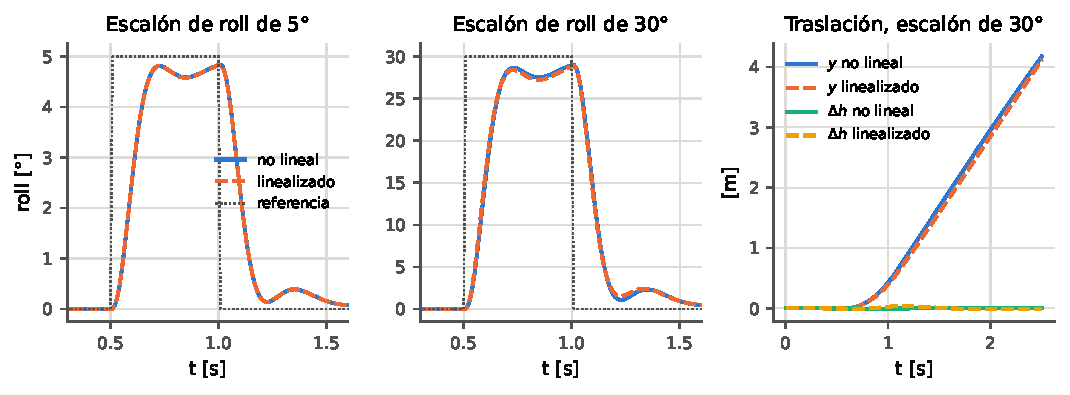
\includegraphics[width=\textwidth]{lineal_vs_no_lineal.pdf}
\caption{Lazo cerrado con la planta no lineal y con la linealizada en hover.
Izquierda y centro: escalones de roll de 5$^\circ$ y 30$^\circ$. Derecha:
desplazamiento lateral y cambio de altura durante el escalón de 30$^\circ$.}
\label{fig:linnl}
\end{figure}

La lectura es la esperada y, por eso, informativa. Hasta 5$^\circ$ las dos
plantas son indistinguibles (diferencias del \val{F2rel} y \val{F5rel}~\%); a
15$^\circ$ la diferencia en roll es del \val{F15rel}~\% y a 30$^\circ$ del
\val{F30rel}~\%, y aparece sobre
todo en la vuelta a cero, donde la proyección $\cos\phi$ del empuje y el
acoplamiento con la altura empiezan a pesar. El modelo no lineal recupera
la linealización en su dominio de validez, y se separa de ella de forma
gradual y con el signo correcto fuera de él. Que la 3.ª edición use el
modelo completo importa justamente en la figura en 8 rápida
(\cref{sec:posicion}), con inclinaciones de hasta \val{lemRTilt}$^\circ$.

\section{Sensores}
\label{sec:sensores}

El controlador no ve el estado; ve medidas. Un simulador que le entrega el
estado verdadero al controlador permite sintonías que el dron real no
tolera, porque oculta el ruido que amplifica el derivativo, el retardo que
come margen de fase y la vibración que satura los motores. El módulo
\cod{sensors.py} modela los sensores del proyecto PAE con valores de hoja de
datos, y cada medida se construye como
\begin{equation}
\text{medida} = \text{verdad} + \text{sesgo} + \text{ruido blanco} + \text{vibración},
\quad \text{entregada con retardo y a su propia tasa.}
\end{equation}
La IMU se muestrea a la tasa del lazo de control (\val{ctrlHz}~Hz,
$\Delta t=2$~ms).

\subsection{Ruido blanco y la densidad espectral}

Las hojas de datos dan el ruido como densidad espectral $N$ (unidad
por $\sqrt{\text{Hz}}$). Muestreado a $f_s$ con ancho de banda igual a
Nyquist, la desviación por muestra es
\begin{equation}
\sigma = N\sqrt{f_s/2} = N\sqrt{1/(2\Delta t)} .
\label{eq:ruido}
\end{equation}
Con los valores de la \cref{tab:sensores}, a 500~Hz el giroscopio tiene
$\sigma=\val{sgGyro}$~$^\circ$/s y el acelerómetro
$\sigma=\val{sgAccmg}$~m$g$ (\val{sgAcc}~m/s$^2$). Son cifras pequeñas: en un
dron real el ruido propio del MEMS lo tapa la vibración, y por eso esta es
configurable por separado.

\begin{table}[H]
\centering
\small
\caption{Parámetros de los sensores (\cod{SensorConfig}).}
\label{tab:sensores}
\begin{tabularx}{\textwidth}{>{\raggedright\arraybackslash}p{3.4cm}>{\raggedright\arraybackslash}X>{\raggedright\arraybackslash}p{4.6cm}}
\toprule
Sensor & Modelo & Fuente del valor \\
\midrule
Giroscopio (ISM330DHCX) & ruido $5$~m$^\circ$/s/$\sqrt{\text{Hz}}$; sesgo inicial $\mathcal N(0,0.3^\circ/\text{s})$ por eje; deriva de sesgo (paseo aleatorio) $0.005^\circ$/s/$\sqrt{\text{s}}$; retardo 2~ms & ruido: hoja de datos DS13012 \cite{ism330}; sesgo y deriva: supuestos típicos \\
Acelerómetro (ISM330DHCX) & ruido $60~\mu g/\sqrt{\text{Hz}}$; sesgo constante $\mathcal N(0,0.05~\text{m/s}^2)$; retardo 2~ms & ruido: DS13012; sesgo: supuesto \\
Vibración de hélices & $3^\circ$/s (giro) y 1.5~m/s$^2$ (acel.) a la velocidad de hover, 2 palas & supuesto (\cref{sec:vibracion}) \\
Magnetómetro (MMC5983MA) & $\vect m_B=\R\T\vect m_E+\vect b_{EMI}+\mathcal N(0,0.04~\mu\text{T})$, 100~Hz & ruido 0.4~mG RMS, hoja de datos \cite{mmc5983} \\
Barómetro (BMP180) & $h+$deriva$+\mathcal N(0,0.17~\text{m})$, 40~Hz, retardo 30~ms, deriva $0.002$~m/$\sqrt{\text{s}}$ & 0.02~hPa RMS en ultra alta resolución \cite{bmp180} $\approx0.17$~m; tasa, retardo y deriva: supuestos \\
Posición externa (mocap/RTK) & $\vect p+\mathcal N(0,0.01~\text{m})$, 100~Hz, retardo 10~ms & supuesto; Larotta \cite{larotta24} usa un sistema externo de este tipo \\
\bottomrule
\end{tabularx}
\end{table}

\paragraph{Sesgo del giroscopio.} El sesgo inicial se sortea una vez por
semilla y luego deriva como paseo aleatorio,
$b_{k+1}=b_k+\mathcal N(0,\sigma_{bw}\sqrt{\Delta t})$. Un sesgo de
$0.3^\circ$/s parece poco, pero integrado sin corrección son $18^\circ$ en un
minuto: es la razón de ser de los estimadores de la \cref{sec:estimadores}.

\subsection{Vibración a la frecuencia de paso de pala}
\label{sec:vibracion}

Cada hélice de dos palas ligeramente desbalanceada sacude el bastidor dos
veces por vuelta. El simulador lleva la fase $\varphi_i$ de cada rotor
(integrada con $\Omega_i$ en cada subpaso de física) y suma al giroscopio y
al acelerómetro
\begin{equation}
\delta\vect\omega_{vib} = A_g\sum_{i=1}^4\left(\frac{\Omega_i}{\Omega_h}\right)^2\sin(n_b\varphi_i)\,\vect d_i,
\qquad
\delta\vect a_{vib} = A_a\sum_{i=1}^4\left(\frac{\Omega_i}{\Omega_h}\right)^2\sin(n_b\varphi_i)\,\vect d'_i,
\label{eq:vib}
\end{equation}
con $n_b=2$ palas, $A_g=3^\circ$/s, $A_a=1.5$~m/s$^2$, $\vect d_i$ una
dirección unitaria aleatoria fija por rotor y $\vect d'_i$ la misma dirección
con las componentes permutadas cíclicamente. La amplitud escala con
$\Omega^2$ porque la fuerza centrífuga de un desbalance de masa crece con el
cuadrado de la velocidad. La frecuencia del tono es
\begin{equation}
f_{bp}=\frac{n_b\,\Omega}{2\pi}=\val{fbp}~\text{Hz en hover}.
\end{equation}

\paragraph{Por qué importa a 500~Hz.} Con la IMU muestreada a 500~Hz el
límite de Nyquist es 250~Hz. En hover el tono de 177~Hz cae por debajo y
se ve tal cual; la densidad espectral del giroscopio simulado
(\cref{fig:psd}) tiene su pico en \val{psdPeak}~Hz, y la frecuencia media que
reporta el simulador es \val{fvib}~Hz. El tono se mueve con el acelerador, y
para $\sigma>\val{sigNyq}$ ($\Omega>\val{wNyq}$~rad/s) pasa de Nyquist y se
\emph{repliega}: a acelerador máximo, los \val{fbpmax}~Hz reales aparecen a
$500-320.4=\val{alias}$~Hz (medido: \val{aliasMeas}~Hz). Un filtro notch fijo
deja de servir justo cuando el dron más exige a sus motores. Los
autopilotos comerciales muestrean el giroscopio a 1--8~kHz por esa razón; el
lazo de 500~Hz del firmware ESP32 del proyecto obliga a convivir con el
problema, y el simulador permite estudiarlo.

\begin{figure}[H]
\centering
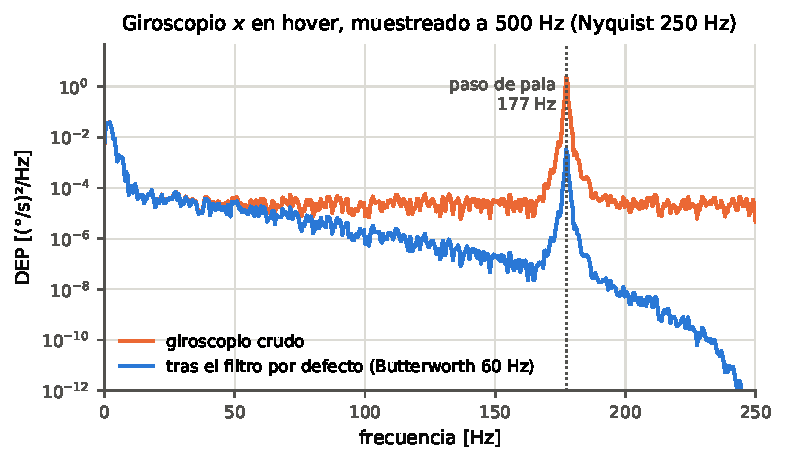
\includegraphics[width=0.78\textwidth]{psd_giroscopio_vibracion.pdf}
\caption{Densidad espectral del giroscopio $x$ en hover (simulador completo,
9~s, 500~Hz). El RMS del giroscopio crudo es \val{rmsRaw}~$^\circ$/s y, tras
el filtro por defecto (\val{filtroDef}), \val{rmsFilt}~$^\circ$/s.}
\label{fig:psd}
\end{figure}

\begin{supuesto}[Amplitud de la vibración]
Las amplitudes $A_g$ y $A_a$ y el espectro de un solo tono por rotor son
supuestos de orden de magnitud. El estudio de barridos (\cref{sec:barridos})
muestra que las conclusiones cualitativas sobre filtros no dependen de ellas,
pero los valores óptimos sí: antes de transferir una sintonía de filtro al
dron real hay que medir su espectro en hover y ajustar $A_g$.
\end{supuesto}

\subsection{Campo magnético}

El campo terrestre en NED geográfico se construye con intensidad $F$,
inclinación $I$ (positiva hacia abajo) y declinación $D$:
\begin{equation}
\vect m_E = F\,\big(\cos I\cos D,\ \cos I\sin D,\ \sin I\big)
= (\val{magN},\ \val{magE},\ \val{magD})~\mu\text{T},
\label{eq:magE}
\end{equation}
con $F=\val{magF}~\mu$T, $I=+\val{magI}^\circ$ y $D=\val{magDecl}^\circ$: el
World Magnetic Model 2025 evaluado para Valledupar (10.46$^\circ$N,
73.25$^\circ$O, unos 170~m de altura), la ciudad más cercana a la sede La
Paz, en la fecha 2026.75 (paquete \cod{pygeomag}). El campo cambia
lentamente con los años; para otra fecha o lugar se recalcula con el mismo
modelo o con la calculadora de NOAA. El EKF usa la misma inclinación para su
referencia magnética. La interferencia $\vect b_{EMI}$ la pone el módulo de
perturbaciones (\cref{sec:perturbaciones}) y afecta solo a la medida: el dron
no la siente, el estimador sí.

\subsection{Retardos y tasas}

Cada sensor tiene una línea de retardo (\cod{\_Delay}) de
$n=\max(1,\operatorname{round}(\tau/\Delta t))$ muestras de control: \val{dImu}
para la IMU, \val{dPos} para la posición externa y \val{dBaro} para el
barómetro. Magnetómetro, barómetro y posición se actualizan a su tasa y
mantienen el último valor entre actualizaciones; cada muestra lleva un
indicador \cod{*\_new} para que los estimadores solo corrijan con datos
nuevos.

\begin{nota}[Inicialización de las líneas de retardo]
Las líneas de retardo de la posición y del barómetro se construyen llenas
con el origen y altura cero, lo correcto para un despegue desde el suelo. Si
la simulación arranca en el aire (\cod{start\_airborne=True}),
\cod{Simulation.\_prime\_airborne} llama a \cod{SensorSuite.prime(x)}, que las
llena con el estado inicial; sin ese paso, durante los primeros 10~ms
(posición) y 30~ms (barómetro) los sensores reportarían ``dron en el origen,
en el suelo'' y el filtro de navegación saltaría la altura completa.
\end{nota}

\section{Filtros digitales del giroscopio}
\label{sec:filtros}

\subsection{Dónde están y qué filtran}

La señal de tasa que llega al PID es la salida del estimador de actitud
(giroscopio menos sesgo estimado) pasada por una cadena de filtros por eje
(\cod{Simulation.step\_control}). Por defecto la cadena tiene dos etapas:
la etapa 0 es un pasa-bajos \val{filtroDef} y la etapa 1, un notch centrado en
177~Hz con $Q=\val{notchQ}$ que viene \val{notchDef}. El corte de
\val{filtroDefFc}~Hz (la 2.ª edición y las primeras versiones de este núcleo
usaban 80~Hz) se fijó junto con el derivativo del lazo de tasa a partir del
barrido conjunto de la \cref{sec:barridos}: un corte más bajo quita más
vibración y su retardo adicional lo compensa el adelanto de fase de un $k_d$
mayor (\cref{sec:control}). El estimador de actitud recibe el giroscopio
sin filtrar, como en PX4, porque integra la tasa y la integral de un tono de
177~Hz es despreciable. El \emph{acelerómetro}, en cambio, sí se filtra antes
del estimador, con un Butterworth de \val{accLpf}~Hz
(\cod{SimConfig.ahrs\_accel\_lpf\_hz}), por la razón no lineal que explica
la \cref{sec:estimadores}.

Todo filtro introduce retardo. El compromiso que el usuario debe resolver,
y que los barridos automáticos de la \cref{sec:barridos} cuantifican, es
cuánto ruido quitar a cambio de cuánto margen de fase perder en el lazo de
tasa.

\subsection{El biquad}

Todos los tipos son secciones de segundo orden (\emph{biquad}) en forma
directa II transpuesta, con los coeficientes del \emph{Audio EQ Cookbook} de
Bristow-Johnson \cite{rbj}, que corresponden a la transformación bilineal
con la frecuencia de corte pre-distorsionada. Es el mismo filtro de
Betaflight y PX4 sobre el giroscopio. La ecuación en diferencias
(\cod{Biquad.process}) es
\begin{equation}
y_k = b_0x_k + z_1,\qquad
z_1 \leftarrow b_1x_k - a_1y_k + z_2,\qquad
z_2 \leftarrow b_2x_k - a_2y_k ,
\label{eq:df2t}
\end{equation}
con $H(z)=\dfrac{b_0+b_1z^{-1}+b_2z^{-2}}{1+a_1z^{-1}+a_2z^{-2}}$. Llamando
$\omega_0=2\pi f_c/f_s$ y $\alpha=\sin\omega_0/(2Q)$, y normalizando por
$a_0=1+\alpha$:
\begin{align}
\text{común:}\quad & a_1=\tfrac{-2\cos\omega_0}{a_0},\qquad a_2=\tfrac{1-\alpha}{a_0};\nonumber\\
\text{pasa-bajos:}\quad & b_0=b_2=\tfrac{1-\cos\omega_0}{2a_0},\qquad b_1=\tfrac{1-\cos\omega_0}{a_0};\label{eq:lpf}\\
\text{notch:}\quad & b_0=b_2=\tfrac{1}{a_0},\qquad b_1=\tfrac{-2\cos\omega_0}{a_0}.\label{eq:notch}
\end{align}

\paragraph{Tipos.} \textbf{Butterworth} es el pasa-bajos con $Q=1/\sqrt2$
(máximamente plano). \textbf{Pasa-bajos} deja libre el $Q$: con $Q>0.707$
el filtro tiene un pico antes del corte pero menos retardo en la banda de
paso. \textbf{Chebyshev~I} de orden 2 con rizado $r_p$~dB: con
$\varepsilon=\sqrt{10^{r_p/10}-1}$ y $v_0=\operatorname{asinh}(1/\varepsilon)/2$,
el polo analógico normalizado es
$s=-\sinh v_0\sin\frac{\pi}{4}\pm j\cosh v_0\cos\frac{\pi}{4}$; de su módulo
$\omega_n$ y su parte real se obtienen $Q=\omega_n/(2|\Re s|)$ y la frecuencia
de diseño $f_c\,\omega_n$, y con ellas se usa \eqref{eq:lpf}. Para 1~dB
resulta $Q=\val{chQ}$. El código normaliza la ganancia continua a 0~dB (la
verificación da 0.0~dB en continua y un máximo de $+1.0$~dB en la banda de
paso): el rizado queda \emph{por encima} de la
ganancia unitaria, a diferencia del Chebyshev de libro de orden par, que
tiene $-r_p$~dB en continua. \textbf{Notch} rechaza una banda angosta
alrededor de $f_c$, tanto más angosta cuanto mayor es $Q$.

\paragraph{Detalles de robustez.} $f_c$ se acota a $0.98$ veces Nyquist y
$Q\ge0.05$; \cod{reset(x0)} inicializa el estado en el régimen permanente de
una entrada constante (sin transitorio de arranque); \cod{Simulation.set\_filter},
que rediseña un filtro en pleno vuelo (desde la GUI o un barrido), lo reinicia
así con la tasa actual, para que el cambio no produzca un escalón en la
señal; si la salida no es finita, el filtro se reinicia y deja pasar la
entrada.

\subsection{Compromiso atenuación--retardo}

La \cref{tab:filtros} y la \cref{fig:bode} comparan, a $f_s=500$~Hz, el
retardo de grupo en 10~Hz (la zona donde vive la dinámica del lazo de tasa)
con la atenuación en la frecuencia de paso de pala.

\begin{table}[H]
\centering
\small
\caption{Retardo y atenuación de los filtros (calculados de la respuesta en
frecuencia exacta de cada biquad, \cod{Biquad.response}).}
\label{tab:filtros}
\begin{tabular}{lccc}
\toprule
Filtro & Retardo de grupo & Fase & Atenuación \\
 & a 10~Hz [ms] & a 10~Hz [$^\circ$] & a 177~Hz [dB] \\
\midrule
Butterworth 80~Hz & \val{gdBWo} & \val{phBWo} & \val{atBWo} \\
Butterworth 60~Hz & \val{gdBWs} & \val{phBWs} & \val{atBWs} \\
Pasa-bajos 40~Hz, $Q=0.707$ & \val{gdLPc} & \val{phLPc} & \val{atLPc} \\
Chebyshev~I 80~Hz, 1~dB & \val{gdCH} & \val{phCH} & \val{atCH} \\
Notch 177~Hz, $Q=4$ & \val{gdNO} & \val{phNO} & $<-200$ (cero exacto) \\
\bottomrule
\end{tabular}
\end{table}

\begin{figure}[H]
\centering
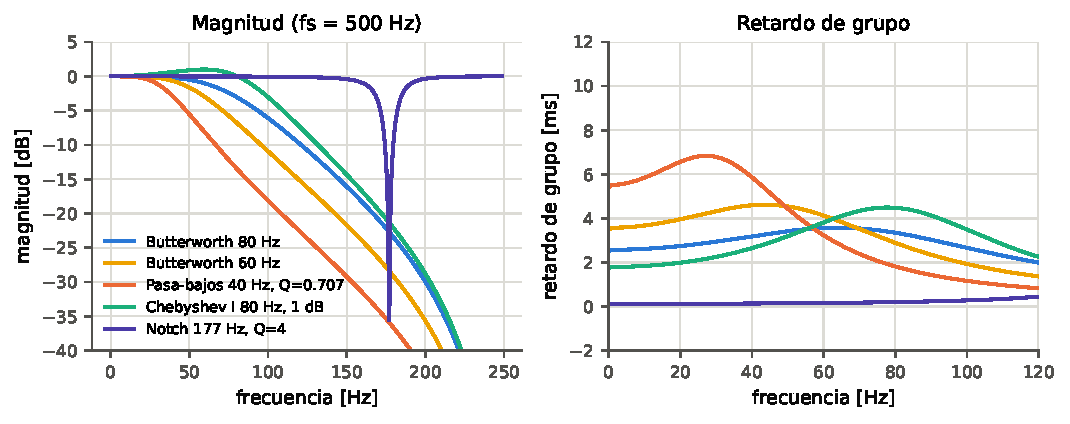
\includegraphics[width=\textwidth]{filtros_bode.pdf}
\caption{Magnitud y retardo de grupo de los filtros de la \cref{tab:filtros}.}
\label{fig:bode}
\end{figure}

Bajar el corte de 80 a 60~Hz gana 6~dB de atenuación de la vibración a
cambio de 1~ms de retardo; bajarlo a 40~Hz gana 13~dB y duplica el retardo. El notch, en cambio, anula el tono con un retardo más de diez
veces menor que cualquier pasa-bajos, pero solo si está centrado: en la
\cref{sec:barridos} se mide que un notch angosto descentrado 2~Hz pierde casi
todo su beneficio, y el tono se mueve con el acelerador
(\cref{sec:vibracion}).

\subsection{Filtro de primer orden}

El término derivativo del PID usa un filtro de primer orden discreto
(\cod{control/pid.py}, y la clase \cod{PT1} de \cod{filters.py}):
\begin{equation}
y_k = y_{k-1}+\alpha\,(x_k-y_{k-1}),\qquad \alpha=\frac{\Delta t}{\tau+\Delta t},\quad \tau=\frac{1}{2\pi f_c}.
\label{eq:pt1}
\end{equation}

\section{Estimadores de actitud y de navegación}
\label{sec:estimadores}

\subsection{El problema que resuelven}

El giroscopio mide bien los cambios rápidos de actitud pero deriva: su
sesgo, integrado, crece sin límite. El acelerómetro y el magnetómetro dan
referencias absolutas (dirección de la gravedad y del norte magnético) pero
ruidosas, perturbables y, en el caso del acelerómetro de un multirrotor,
engañosas, como se verá enseguida. Un estimador de actitud (AHRS) fusiona
las tres fuentes. El simulador ofrece cuatro, intercambiables en caliente
(\cod{estimators.py}): \emph{ideal} (devuelve la verdad, sirve de línea
base), Madgwick, Mahony y un filtro de Kalman extendido. El estimador por
defecto es \val{estDef} (\cod{SimConfig.estimator}): con el acelerómetro
filtrado fue el más equilibrado entre escalones de actitud, maniobras y
seguimiento de trayectoria. Los tres reales comparten tres convenciones:
\begin{itemize}
\item la dirección de la gravedad medida en el cuerpo es
$\hat{\vect s}_g=-\vect a/\|\vect a\|$ (en reposo el acelerómetro lee
$(0,0,-g)$ en FRD);
\item trabajan en un NED magnético y rotan la salida por la declinación
(\cref{sec:marcos});
\item se inicializan con la primera muestra (\cod{triad\_alignment}): roll
y pitch del acelerómetro,
$\phi_0=\operatorname{atan2}(-a_y,-a_z)$,
$\theta_0=\operatorname{atan2}\big(a_x,\sqrt{a_y^2+a_z^2}\big)$, y rumbo del
magnetómetro compensado por inclinación,
$\psi_0=\operatorname{atan2}(-m_{h,y},m_{h,x})+D$, con
$m_{h,x}=m_x\cos\theta_0+m_y\sin\phi_0\sin\theta_0+m_z\cos\phi_0\sin\theta_0$ y
$m_{h,y}=m_y\cos\phi_0-m_z\sin\phi_0$.
\end{itemize}

\begin{nota}[Inicialización en el aire]
Si la simulación arranca en vuelo, la primera muestra trae la vibración de
las hélices (hasta 1.5~m/s$^2$) y alinear con ella dejaba errores iniciales
de varios grados ($\approx9^\circ$ de cabeceo medidos con Madgwick). Con
\cod{start\_airborne=True}, \cod{Simulation.\_prime\_airborne} inicializa el
estimador con la actitud verdadera. Es la hipótesis coherente con ``arrancar
en el aire'': el autopiloto real se alinea en tierra, con los motores
apagados, antes de despegar, y llega al vuelo con el estimador convergido.
Los sesgos y el ruido de los sensores se conservan; no es el estimador ideal.
\end{nota}

\subsection{El acelerómetro de un multirrotor no mide la gravedad}
\label{sec:leishman}

La \eqref{eq:fesp} dice que el acelerómetro mide
$\vect f_{acc}=(\vect f_B+\R\T\vect F_{ext})/m$: empuje más arrastre. En
vuelo estacionario inclinado $15^\circ$ y sin velocidad, el modelo da
$\vect f_{acc}=(0,\ 0,\ -9.80665)$, exactamente igual que nivelado: el roll
aparente que deduce el acelerómetro es $0^\circ$. Leishman, Macdonald, Beard
y McLain \cite{leishman14} lo explican con detalle: la idea de que el
acelerómetro ``mide la gravedad cuando no hay aceleración'' falla en un
multirrotor, porque inclinado \emph{siempre} acelera horizontalmente (salvo
que el arrastre lo equilibre), y lo que mide es la fuerza del rotor, alineada
con $z_B$.

La consecuencia práctica es que, durante una aceleración sostenida, un AHRS
que trate $-\vect a/\|\vect a\|$ como gravedad converge a ``nivelado'' y el
lazo de actitud, que cree estar en el ángulo pedido, sigue inclinando el
dron. El simulador implementa la corrección que usa PX4 (\cod{ATT\_ACC\_COMP}):
restar al acelerómetro la aceleración cinemática estimada por el filtro de
navegación antes de pasarlo al AHRS (\cod{SimConfig.acc\_compensation},
activa por defecto con el dron armado y, como se explica más abajo, solo
cuando el filtro de navegación recibe correcciones de posición absoluta). La
cadena completa del acelerómetro
hacia el AHRS (\cod{Simulation.step\_control}) es, por eje,
\begin{gather}
\vect a_{kin,E} = \operatorname{sat}_{0.8g}\Big(\mathcal{H}_{\val{accLpf}}\Big\{\frac{\hat{\vect v}_k-\hat{\vect v}_{k-1}}{\Delta t}\Big\}\Big),\label{eq:akin}\\
\vect a_{AHRS} = \mathcal{H}_{\val{accLpf}}\{\vect a_{med}\} - \kappa\,\hat\R\T\vect a_{kin,E},\qquad \kappa\in[0,1],\label{eq:acomp}
\end{gather}
con $\mathcal H_{\val{accLpf}}$ un Butterworth de segundo orden de
\val{accLpf}~Hz (\cod{SimConfig.ahrs\_accel\_lpf\_hz}; 0 lo desactiva), que
quita la vibración antes de la normalización $\vect a/\|\vect a\|$
(\cref{sec:rectificacion}). La derivada de la velocidad estimada pasa por el
\emph{mismo} Butterworth que el acelerómetro, para que las dos señales que se
restan lleguen con el mismo retardo, y su norma se recorta a $0.8g$. La
ganancia $\kappa$ de la compensación sube o baja en rampa en 0.5~s
(\cod{acc\_comp\_ramp\_s}), de modo que activarla o perderla en vuelo no
produce un salto. Todo esto vive en \cod{quadsim/estimation.py}, una sola
cadena que usan la simulación y los barridos de estimadores. La rotación que
aparece en \eqref{eq:acomp} es
la \emph{estimada}, $\hat\R$, y no la verdadera: el AHRS no conoce otra. La
edición anterior escribía el resultado como $\approx-g\,\R\T\eu$, y esa
lectura solo vale si $\vect a_{kin,E}$ es la aceleración real medida por una
vía independiente del acelerómetro y $\hat\R\approx\R$. En ese caso, con
$\vect f_{acc}=\R\T(\dot{\vect v}-g\eu)$,
\[
\vect a_{AHRS}\approx\R\T(\dot{\vect v}-g\eu)-\hat\R\T\dot{\vect v}\approx-g\,\R\T\eu ,
\]
y el AHRS recibe la dirección verdadera de la gravedad. El problema es de
dónde sale $\vect a_{kin,E}$. El filtro de navegación predice con el
\emph{mismo} acelerómetro rotado con la actitud estimada,
$\vect a_E=\hat\R\vect f_{acc}+g\eu$ (\cref{eq:nav}). Entre correcciones de
posición, entonces, $\vect a_{kin,E}\approx\hat\R\vect f_{acc}+g\eu$ y
\[
\vect a_{AHRS}\approx\vect f_{acc}-\hat\R\T\big(\hat\R\vect f_{acc}+g\eu\big)=-g\,\hat\R\T\eu :
\]
el AHRS recibe su propia estimación de la gravedad. La compensación es
\emph{autorreferente}. La información real de gravedad solo entra a través
del término de corrección del filtro de navegación, es decir, de las medidas
de posición. Sin sensor de posición (solo barómetro, que no corrige el plano
horizontal) roll y pitch dejan de ser observables, y con ellos el sesgo del
giroscopio. La revisión externa lo reprodujo con Mahony en 30~s de vuelo
estacionario, partiendo de una alineación perfecta: con sensor de posición y
compensación el error de inclinación fue 0.45$^\circ$; solo con barómetro y
compensación creció a 15.2$^\circ$ (unos 0.5$^\circ$/s) con 157~m de deriva
horizontal; solo con barómetro y sin compensación quedó en 1.4$^\circ$.

De ahí la regla que aplica el núcleo (\cod{AccelCompensation.wanted}): la
compensación actúa solo si hubo una corrección \emph{horizontal} de posición
absoluta en los últimos 0.2~s (\cod{acc\_comp\_fix\_timeout\_s}), si el dron
está armado y en el aire y si el filtro de navegación ya se asentó (tras
\cod{settle} o 1~s después de un reinicio). En tierra, recién armado, la
velocidad del navegador reiniciado producía una $\vect a_{kin,E}$ espuria de
1.6--2.8~m/s$^2$. Además, el filtro de navegación rechaza medidas de
posición atípicas: las que superan 5 desviaciones estándar de la innovación
predicha (\cod{nav\_gate\_sigma}) y, a la vez, se alejan más de 25~cm de la
predicción (\cod{gate\_min\_m}). El piso absoluto evita que una predicción
sesgada, por ejemplo por un rumbo estimado desviado, haga rechazar medidas
buenas una tras otra (\cref{sec:lectura_banco}). Sin correcciones de posición el AHRS recibe el
acelerómetro filtrado sin compensar, que se equivoca durante las
aceleraciones sostenidas pero no deriva: en el mismo vuelo estacionario de
30~s, solo con barómetro, el error de inclinación pasó de 15.2 a
1.46$^\circ$ (prueba \cod{test\_baro\_only\_hover\_keeps\_tilt\_estimate}). Es la situación del dron
real del proyecto (ESP32 con BMP180 y sin captura de movimiento), así que la
compensación, tal como está, no le sirve: haría falta estimar
$\vect a_{kin,E}$ por una vía independiente (por ejemplo, la segunda
derivada filtrada de una posición medida o la aceleración de referencia de
la trayectoria) o una arquitectura acoplada en la que el error de actitud sea
estado del filtro de navegación, como el EKF2 de PX4.

Hay un segundo límite, de sincronía. La versión anterior suavizaba
$\vect a_{kin,E}$ con un filtro de primer orden fijo de 50~ms, que no dependía
de \cod{ahrs\_accel\_lpf\_hz}, y la calculaba después del AHRS, de modo que se
usaba un periodo tarde; el desfase frente a la ruta del acelerómetro era de
65.6~ms. Con el mismo Butterworth en las dos ramas y el cálculo antes del
AHRS bajó a 17.0~ms. Lo que queda es el atraso propio de la velocidad del
navegador: la posición llega con 10~ms de retardo y se fusiona como si fuera
actual.

El filtrado suaviza la derivada de la velocidad
estimada, que es ruidosa; la misma $\vect a_{kin,E}$ se entrega a los
controladores de posición en \cod{NavState.acc}. El filtro de navegación,
en cambio, predice con el acelerómetro sin filtrar
(\cref{eq:nav}).

\begin{figure}[H]
\centering
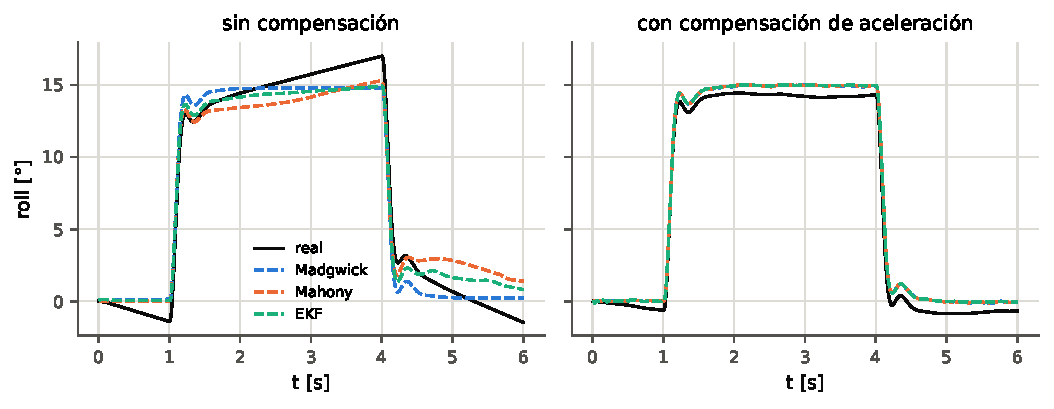
\includegraphics[width=\textwidth]{estimadores_aceleracion.pdf}
\caption{Roll real y estimado durante una inclinación sostenida de
$15^\circ$ (de $t=1$ a 4~s), sin y con compensación de aceleración.}
\label{fig:acc}
\end{figure}

La \cref{fig:acc} y la \cref{tab:acc} muestran el efecto. Sin compensación,
Mahony y el EKF ``ven'' 15$^\circ$ mientras el dron real llega a unos
31--34$^\circ$; con compensación el error máximo de los tres queda por debajo
de 1$^\circ$. Madgwick sin compensación se equivoca poco
(\val{mmadSe}$^\circ$) por una razón que no es mérito: con $\beta=\val{betaDef}$
su corrección por gravedad es tan lenta que en 3~s apenas se aparta de la
integración del giroscopio. Esa misma lentitud es la que lo atrasa en
maniobras largas.

\begin{table}[H]
\centering
\small
\caption{Inclinación sostenida de $15^\circ$ durante 3~s (bloque I):
error máximo del roll estimado y roll real al final del tramo.}
\label{tab:acc}
\begin{tabular}{lcccc}
\toprule
& \multicolumn{2}{c}{Sin compensación} & \multicolumn{2}{c}{Con compensación} \\
\cmidrule(lr){2-3}\cmidrule(lr){4-5}
Estimador & error máx [$^\circ$] & roll real [$^\circ$] & error máx [$^\circ$] & roll real [$^\circ$] \\
\midrule
Madgwick & \val{mmadSe} & \val{mmadSr} & \val{mmadCe} & \val{mmadCr} \\
Mahony   & \val{mmahSe} & \val{mmahSr} & \val{mmahCe} & \val{mmahCr} \\
EKF      & \val{mekfSe} & \val{mekfSr} & \val{mekfCe} & \val{mekfCr} \\
\bottomrule
\end{tabular}
\end{table}

\subsection{Madgwick}

Madgwick, Harrison y Vaidyanathan \cite{madgwick11} plantean la corrección
como un paso de descenso por gradiente sobre el error entre direcciones
medidas y predichas. Con $\vect d$ una dirección de referencia en $\E$ y
$\vect s$ su medida en $\B$, el residuo es $\vect f(\vect q)=\R(\vect q)\T\vect d-\vect s$
y su jacobiano analítico (\cod{\_jac\_rot\_inv}), con $\vect q=(w,\vect u)$:
\begin{equation}
\frac{\partial(\R\T\vect d)}{\partial w}=-2\,\vect u\times\vect d,\qquad
\frac{\partial(\R\T\vect d)}{\partial\vect u}=2w\,\sk{\vect d}+2\big((\vect u\cdot\vect d)I+\vect u\vect d\T-2\vect d\vect u\T\big).
\label{eq:jacmad}
\end{equation}
El código usa dos pares: gravedad, $\vect d_g=\eu$ con $\vect s=\hat{\vect s}_g$;
y campo magnético, $\vect d_m=\vect b$ con $\vect s=\hat{\vect m}$, donde la
referencia se reconstruye de la propia medida:
$\vect h=\R\hat{\vect m}$, $\vect b=(\sqrt{h_x^2+h_y^2},\,0,\,h_z)$. La
actualización (\cod{MadgwickEstimator.update}) es
\begin{equation}
\nabla=\sum_j J_j\T\vect f_j,\qquad
\dot{\vect q}=\tfrac12\vect q\otimes[0,\vect\omega_{med}]-\beta\,\frac{\nabla}{\|\nabla\|},\qquad
\vect q\leftarrow\frac{\vect q+\dot{\vect q}\,\Delta t}{\|\vect q+\dot{\vect q}\,\Delta t\|},
\label{eq:madgwick}
\end{equation}
con $\beta=\val{betaDef}$~rad/s por defecto. Dos rasgos importan al
interpretar resultados. El primero es que el paso de corrección está
\emph{normalizado}: su magnitud es siempre $\beta$, sea grande o pequeño el
error. Con un acelerómetro limpio (filtrado y compensado) el término
correctivo se comporta casi como un relé de amplitud $\beta$, y un $\beta$
grande produce un ciclo límite que el lazo de actitud amplifica. Se midió en
lazo cerrado con el núcleo actual: en la figura en 8
con el PID de posición, $\beta=0.1$ da 12.2~cm de RMSE, $\beta=0.03$ da
4.1~cm y $\beta=0.015$, 2.7~cm; en el escalón de roll, $\beta=0.12$ deja
2.5$^\circ$ de error de estimación. Por eso el valor por defecto es pequeño.
El precio es que, en maniobras sostenidas agresivas, el estimador se
atrasa. Este valor no coincide con el óptimo del barrido de $\beta$
(0.10--0.15, \cref{sec:barridos}): aquel barrido midió el error de
estimación \emph{en sombra} con la cadena de entonces, con el acelerómetro
crudo y sin realimentación del estimador sobre el vuelo, y el ciclo límite
solo aparece cuando el estimador cierra el lazo. El segundo rasgo es que esta implementación es la
versión sin compensación de deriva del giroscopio (el término $\zeta$ de la
sec.~3.4 del artículo no está): el sesgo no se estima y \cod{rates()}
entrega el giroscopio crudo.

\subsection{Mahony}

Mahony, Hamel y Pflimlin \cite{mahony08} formulan un filtro complementario
no lineal en $SO(3)$ con acción proporcional e integral. El error es el
producto cruz entre direcciones medidas y predichas:
\begin{equation}
\vect e=\hat{\vect s}_g\times(\R\T\eu)\ +\ \hat{\vect m}\times(\R\T\vect b),
\label{eq:mahony_e}
\end{equation}
con $\vect b$ construido como en Madgwick. La corrección y el integrador
(\cod{MahonyEstimator.update}):
\begin{equation}
\vect I\leftarrow\vect I+k_i\,\vect e\,\Delta t,\qquad
\hat{\vect b}_g=-\vect I,\qquad
\vect\omega_c=\vect\omega_{med}+k_p\vect e+\vect I,\qquad
\vect q\leftarrow\operatorname{norm}\!\big(\vect q+\tfrac12\vect q\otimes[0,\vect\omega_c]\Delta t\big),
\label{eq:mahony}
\end{equation}
con $k_p=\val{mahKp}$~rad/s y $k_i=\val{mahKi}$~rad/s$^2$ por defecto. El
integrador es exactamente el sesgo estimado del giroscopio, con el signo
cambiado, y se recorta al mismo tope que usa el EKF para el sesgo.

\paragraph{Magnetómetro solo para el rumbo.} Tal como están escritas,
\eqref{eq:madgwick} y \eqref{eq:mahony_e} dejan que el magnetómetro corrija
los tres ejes. Con una interferencia fuerte, que tiene componente vertical,
eso inclina también roll y pitch. En Madgwick y Mahony el código proyecta la
corrección magnética sobre el eje vertical terrestre expresado en el
cuerpo, como hace el estimador de actitud de PX4
(\cod{attitude\_estimator\_q}), de modo que el magnetómetro solo mueve el
rumbo. En el escenario \cod{estimator\_accuracy} con 40~$\mu$T de EMI, el
error de inclinación de Mahony bajó de 9.67 a 1.59$^\circ$ RMS y el de
Madgwick de 2.9 a 1.1$^\circ$; sin EMI la proyección cuesta unos
0.03$^\circ$, porque el campo correcto también aportaba algo de información
de inclinación. El EKF no lleva esta proyección.

\subsection{Filtro de Kalman extendido (7 estados)}

El EKF (\cod{EKFEstimator}) usa el estado $\vect x=[\vect q\T,\vect b_g\T]\T$
con formulación aditiva sobre el cuaternión y renormalización, en la línea
de Sabatini \cite{sabatini06}.

\paragraph{Predicción.} Con $\vect\omega=\vect\omega_{med}-\vect b_g$,
\begin{gather}
\bar{\vect q}=\operatorname{norm}\big(\vect q+\Omega(\vect\omega)\vect q\,\Delta t\big),\qquad
\Omega(\vect\omega)=\frac12\begin{bmatrix}0&-\omega_x&-\omega_y&-\omega_z\\
\omega_x&0&\omega_z&-\omega_y\\ \omega_y&-\omega_z&0&\omega_x\\ \omega_z&\omega_y&-\omega_x&0\end{bmatrix},\\
F=\begin{bmatrix}I_4+\Omega\Delta t & -\Xi(\vect q)\Delta t\\ 0 & I_3\end{bmatrix},\qquad
\Xi(\vect q)=\frac12\begin{bmatrix}-q_x&-q_y&-q_z\\ q_w&-q_z&q_y\\ q_z&q_w&-q_x\\ -q_y&q_x&q_w\end{bmatrix},\\
P\leftarrow FPF\T+Q,\qquad Q=\diag\big(\sigma_g^2\Delta t^2\,\Xi\Xi\T,\ \ \sigma_{bw}^2\Delta t\,I_3\big),
\end{gather}
con $\sigma_g=\val{ekfGyro}$~rad/s y $\sigma_{bw}=\val{ekfBias}$~rad/s/$\sqrt{\text{s}}$
por defecto, y $P_0=\diag(10^{-3}I_4,\,10^{-4}I_3)$.

\paragraph{Corrección.} Medidas: la dirección de la gravedad en cada paso, y
la dirección del campo magnético solo cuando hay muestra nueva (100~Hz). A
diferencia de Madgwick y Mahony, la referencia magnética es fija y conocida,
$\vect m_{ref}=(\cos I,0,\sin I)$ en el NED magnético:
\begin{gather}
\vect z=\begin{bmatrix}\hat{\vect s}_g\\ \hat{\vect m}\end{bmatrix},\quad
\vect h(\bar{\vect q})=\begin{bmatrix}\R\T\eu\\ \R\T\vect m_{ref}\end{bmatrix},\quad
H=\begin{bmatrix}J(\bar{\vect q},\eu) & 0\\ J(\bar{\vect q},\vect m_{ref}) & 0\end{bmatrix},\\
R=\diag\big(\sigma_a^2\,(1+k_{ad}\,\big|\|\vect a\|-g\big|/g)^2\,I_3,\ \ \sigma_m^2I_3\big),\\
K=PH\T(HPH\T+R)^{-1},\quad \vect x\leftarrow\vect x+K(\vect z-\vect h),\quad
P\leftarrow\tfrac12\big[(I-KH)P+((I-KH)P)\T\big],
\end{gather}
con $J$ de \eqref{eq:jacmad}, $\sigma_a=\val{ekfAcc}$, $\sigma_m=\val{ekfMag}$
(adimensionales: son ruidos sobre direcciones unitarias) y $k_{ad}=4$. Los
valores de $\sigma_a$ y $\sigma_m$ son los que el barrido de la
\cref{sec:barridos} encontró robustos frente a interferencia magnética; los
primeros valores del núcleo (0.05 y 0.05) confiaban demasiado en un
acelerómetro que la vibración desvía en $1.5/9.8\approx0.15$ de dirección, y
demasiado poco en la medida magnética. El factor adaptativo infla la covarianza del acelerómetro cuando su norma se
aleja de $g$, es decir, en maniobra. Tras la corrección se renormaliza el
cuaternión y el sesgo se acota a $\pm0.2$~rad/s.

\subsection{Resultados en vuelo estacionario}

La \cref{tab:hover_est} resume 10~s de vuelo estacionario en modo actitud
(después de 2~s de asentamiento), con y sin vibración.

\begin{table}[H]
\centering
\small
\caption{Error del estimador en hover, media / desviación estándar
[$^\circ$] (bloque I, semilla 1).}
\label{tab:hover_est}
\begin{tabular}{llccc}
\toprule
Estimador & Vibración & roll & pitch & yaw \\
\midrule
Madgwick & sí & \val{hmadVr} & \val{hmadVp} & \val{hmadVy} \\
         & no & \val{hmadNr} & \val{hmadNp} & \val{hmadNy} \\
Mahony   & sí & \val{hmahVr} & \val{hmahVp} & \val{hmahVy} \\
         & no & \val{hmahNr} & \val{hmahNp} & \val{hmahNy} \\
EKF      & sí & \val{hekfVr} & \val{hekfVp} & \val{hekfVy} \\
         & no & \val{hekfNr} & \val{hekfNp} & \val{hekfNy} \\
\bottomrule
\end{tabular}
\end{table}

Con el núcleo actual los tres estimadores quedan por debajo de
$0.65^\circ$ de error medio y de $0.15^\circ$ de desviación, y los resultados
con y sin vibración son prácticamente iguales: el pasa-bajos del
acelerómetro y el filtro del giroscopio la retiran. El error medio que queda
(0.5--0.6$^\circ$ en roll) es un sesgo lento, del orden de los
$0.3^\circ$ del sesgo inicial del acelerómetro ($0.05/9.8$~rad) más el resto
de la rectificación. Con el núcleo anterior el cuadro era otro: Madgwick
deambulaba con 1--2$^\circ$ de desviación y el EKF con vibración llegaba a
$1.6^\circ$; el paso normalizado de Madgwick con $\beta=0.08$ y el
$\sigma_a=0.05$ del EKF explicaban la diferencia.

\paragraph{Sesgo por rectificación de la vibración.}
\phantomsection\label{sec:rectificacion}
Esta es la razón del pasa-bajos de \eqref{eq:acomp}. La normalización
$\vect a/\|\vect a\|$ es no lineal: si la vibración $\vect n$ de cada rotor
actúa a lo largo de una dirección fija con componentes vertical y horizontal,
el término de segundo orden $-(\vect n\cdot\hat{\vect g})\vect n_\perp/g^2$
tiene media no nula, del orden de $A_a^2/(4g^2)\approx0.34^\circ$ por rotor.
El bloque I2 lo mide desactivando el filtro
(\cod{ahrs\_accel\_lpf\_hz = 0}): el error medio de inclinación (4 semillas,
5~s en hover) es \val{rectmadC}$^\circ$ con Madgwick, \val{rectmahC}$^\circ$
con Mahony y \val{rectekfC}$^\circ$ con el EKF. Con el Butterworth de
\val{accLpf}~Hz del núcleo (el equivalente de \cod{IMU\_ACCEL\_CUTOFF} de
PX4) baja a \val{rectmadF}, \val{rectmahF} y \val{rectekfF}$^\circ$. La
verificación de la 3.ª edición detectó este sesgo y el filtro se incorporó
al núcleo a raíz de ello.

\subsection{Filtro de navegación}

Los controladores de posición necesitan posición y velocidad estimadas.
\cod{NavEstimator} es un Kalman lineal independiente por eje con estado
$[p,v]$, el esqueleto lineal del EKF2 de PX4. Predice con la aceleración
medida llevada al marco inercial con la actitud \emph{estimada},
\begin{equation}
\vect a_E=\hat\R\,\vect a_{med}+g\eu,\qquad
\begin{bmatrix}p\\v\end{bmatrix}_{k+1}=\begin{bmatrix}1&\Delta t\\0&1\end{bmatrix}\begin{bmatrix}p\\v\end{bmatrix}_k+\begin{bmatrix}\Delta t^2/2\\ \Delta t\end{bmatrix}a_E,\qquad
P\leftarrow FPF\T+G\,q_a^2\,G\T,
\label{eq:nav}
\end{equation}
con $q_a=0.5$~m/s$^2$ (\cod{SimConfig.nav\_accel\_noise}, un valor de
diseño que cubre sobre todo la vibración y el error de actitud, no el ruido
blanco del acelerómetro), y corrige con el sensor de posición externo
($\sigma=0.01$~m, tres ejes) cuando llega una muestra nueva o, si no, con
el barómetro ($\sigma=0.17$~m, solo $z$). Un error de actitud de
$\delta$ radianes inyecta $g\,\delta$ de aceleración horizontal falsa en la
predicción: el estimador de navegación hereda los errores del AHRS, y esa
es una de las razones por las que el error de seguimiento depende del
estimador de actitud (\cref{sec:posicion}).

\begin{nota}[Detalles de implementación del filtro de navegación]
\begin{itemize}[leftmargin=1.2em]
\item El barómetro se fusiona aunque el sensor de posición esté activo: la
condición es \emph{posición nueva} o, en su defecto, \emph{barómetro nuevo},
y como las dos tasas no están sincronizadas, en 10~s se registraron
\val{navPos} correcciones de posición y \val{navBaro} de barómetro. El efecto
es despreciable porque $\sigma_{baro}\gg\sigma_{pos}$: el error RMS de la
altura estimada en 60~s es \val{zBaro}~mm con esa fusión y \val{zNoBaro}~mm
sin ella.
\item \cod{reset} deja $P=0.1\,I$; con esa covarianza inicial la ganancia
sobre la velocidad es grande durante unos 0.5~s y la velocidad estimada
tiene 5--8~cm/s de ruido. En un arranque en el aire,
\cod{NavEstimator.settle} itera el propio filtro durante 2~s con la medida
exacta y lleva $P$ a régimen sin cambiar el estado.
\end{itemize}
\end{nota}

\section{Control de bajo nivel}
\label{sec:control}

\subsection{Arquitectura en cascada}

El control de actitud es una cascada de tres niveles, la misma de PX4, del
firmware ESP32 del proyecto y de la descripción que hace Larotta
\cite{larotta24} (p.~57) del Crazyflie (\cod{control/attitude.py}):
\begin{equation}
\underset{\scriptscriptstyle \text{actitud}}{(\phi,\theta,\psi)_{ref}}
\xrightarrow{\ \text{P}\ }
\underset{\scriptscriptstyle \text{tasas de Euler}}{(\dot\phi,\dot\theta,\dot\psi)_{ref}}
\xrightarrow{\ W\ }
\underset{\scriptscriptstyle \text{tasa}}{\vect\omega_{ref}}
\xrightarrow{\ \text{PID}\ }
\underset{\scriptscriptstyle \text{momento norm.}}{u\in[-1,1]^3}
\xrightarrow{\ \times\tau_{max}\ }
\vect\tau
\xrightarrow{\ \text{mezclador}\ }\sigma_{1..4}.
\label{eq:cascada}
\end{equation}
La cascada funciona porque las constantes de tiempo están separadas: el lazo
de tasa ve un integrador rápido (\cref{eq:Krate}) y el de ángulo ve el lazo de
tasa cerrado como un retardo corto. Powers, Mellinger y Kumar \cite{hb16}
(p.~317) lo justifican desde la linealización en hover: a ángulos pequeños
el control de actitud se desacopla del de posición y admite lazos anidados.

\paragraph{Lazo de ángulo.} Proporcional puro sobre el error de cada ángulo
de Euler (el de yaw envuelto a $(-\pi,\pi]$ para girar por el camino corto),
más una prealimentación de tasa de yaw opcional:
\begin{equation}
\dot\phi_{ref}=K_{\phi}(\phi_{ref}-\hat\phi),\quad
\dot\theta_{ref}=K_{\theta}(\theta_{ref}-\hat\theta),\quad
\dot\psi_{ref}=K_{\psi}\operatorname{wrap}(\psi_{ref}-\hat\psi)+\dot\psi_{ff},
\end{equation}
convertido a tasa del cuerpo con \eqref{eq:W} y acotado a $220^\circ$/s en
roll y pitch y $120^\circ$/s en yaw. No lleva integrador: el lazo de tasa
interno ya tiene uno, y un segundo integrador sobre una planta integradora
solo agrega sobreimpulso.

\paragraph{Lazo de tasa.} Un PID por eje (\cod{control/pid.py}) cuya salida
es el momento normalizado $u$; el momento físico es
$\tau=u\,\tau_{max}$ con $\tau_{max}$ de \eqref{eq:taumax}. Normalizar es la
convención de PX4 (\cod{MC\_ROLLRATE\_P} está en momento normalizado por
rad/s) y tiene una ventaja práctica: las ganancias de vehículos con
inercias que difieren en tres órdenes de magnitud quedan en el mismo rango
numérico.

\subsection{El PID discreto}

En cada periodo $\Delta t$ (\cod{PID.update}):
\begin{align}
e_k&=r_k-y_k,\nonumber\\
I_k&=\begin{cases}I_{k-1} & \text{si la salida está saturada y } e_k\,u_{k-1}>0\\
\sat_{\pm i_{lim}/k_i}\!\big(I_{k-1}+e_k\Delta t\big) & \text{en otro caso}\end{cases}\label{eq:pid}\\
d_k&=d_{k-1}+\alpha_d\Big(-\frac{y_k-y_{k-1}}{\Delta t}-d_{k-1}\Big),\qquad \alpha_d=\frac{\Delta t}{\tau_d+\Delta t},\ \tau_d=\frac{1}{2\pi f_d}\nonumber\\
u_k&=\sat_{\pm u_{lim}}\big(k_pe_k+k_iI_k+k_dd_k+k_{ff}r_k\big).\nonumber
\end{align}
Cada protección responde a una falla real. La derivada sobre la
\emph{medida}, y no sobre el error, evita el golpe derivativo cuando la
referencia salta. El filtro del derivativo ($f_d=40$~Hz nominales en el
lazo de tasa) evita que la vibración llegue amplificada a los motores. Se
discretiza como en Betaflight, $\alpha=\Delta t/(\tau+\Delta t)$, y esa
fórmula no da el corte nominal: a 500~Hz el corte efectivo es 32.4~Hz, con
unos 4.9~ms de retardo en baja frecuencia. Se conserva por compatibilidad con
las ganancias afinadas; la opción \cod{d\_filter\_exact} de la clase \cod{PID} usa
$\alpha=1-e^{-2\pi f_d\Delta t}$, cuyo corte coincide con el nominal. Cuál de
las dos usa el firmware del dron está por verificar. La integración
condicional congela el integrador cuando la salida está saturada y el error
empuja hacia el mismo lado (\emph{anti-windup}), y el límite absoluto
$|k_iI|\le i_{lim}=0.3$ acota cuánto momento puede acumular. En el lazo de
tasa $u_{lim}=1$.

\subsection{Sintonía SIMC a partir del modelo}

Las ganancias por defecto no están escritas a mano: \cod{control/tuning.py}
las calcula con las reglas SIMC de Skogestad \cite{skogestad03} a partir de
los parámetros físicos, de modo que cambiar de vehículo cambia las
ganancias. SIMC tiene un solo parámetro libre, la constante de tiempo de
lazo cerrado deseada $\tau_c$, con interpretación física directa; es más
fácil de defender ante evaluadores que una sintonía por optimización de caja
negra, y produce márgenes de robustez razonables por construcción
(Ziegler--Nichols, en comparación, da sobreimpulsos del orden del 25~\%
\cite{astrom04}).

\paragraph{Modelo de diseño del lazo de tasa.} Linealizando en hover
(\cref{sec:linealizacion}) cada eje es un integrador, y los retardos de la
cadena se agrupan con la ``regla de la mitad'' de SIMC (la mitad de la
constante de tiempo despreciada se suma al retardo):
\begin{equation}
\frac{\omega(s)}{u(s)}=\frac{K\,e^{-\theta s}}{s},\qquad
K=\frac{\tau_{max}}{J},\qquad
\theta=\underset{\scriptscriptstyle 2\ \text{ms}}{\tau_{IMU}}+\underset{\scriptscriptstyle 1\ \text{ms}}{\Delta t/2}+\underset{\scriptscriptstyle 3\ \text{ms}}{\tau_{filtro}}+\underset{\scriptscriptstyle 10\ \text{ms}}{T_m/2}=\val{theta}~\text{ms}.
\label{eq:simc_planta}
\end{equation}
Esa es la cadena \emph{nominal} con la que se afinaron y documentaron las
ganancias por defecto: 2~ms de IMU y 3~ms fijos de filtro, el retardo del
Butterworth de 80~Hz de las primeras versiones (\val{gdBWo}~ms de retardo de
grupo a 10~Hz, \cref{tab:filtros}). Con el filtro actual, \val{filtroDef}, el
retardo de grupo a 10~Hz es \val{defGd10}~ms. \cod{chain\_delay} también sabe
leer la cadena \emph{configurada} (\cod{Simulation.attitude\_chain}): retardo
de la IMU de \cod{SensorConfig}, retardo de grupo de las etapas de filtro de
cada eje evaluado en el cruce estimado (que depende de $\theta$ y se
resuelve por punto fijo), retardo de cómputo y retardo del ESC. Con la
configuración por defecto da $\theta=16.6$~ms en lugar de 16.0, y un $K_p$ de
tasa 3.6~\% menor. La simulación solo usa la cadena configurada si se pide
(\cod{SimConfig.gains\_from\_chain}), para que las ganancias no cambien en
silencio durante un barrido de filtros, donde el filtro varía con las
ganancias fijas. Dos cosas quedan fuera de $\theta$ por diseño: el filtro del
derivativo, que solo afecta a esa rama, y la forma exacta del rezago del
motor. La regla de la mitad reparte $T_m/2=10$~ms, cuando el motor de primer
orden aporta en la frecuencia de cruce más fase que esa. Las ganancias SIMC
son, por eso, un punto de partida; los márgenes reales del lazo se discuten
en la \cref{sec:integracion}. Para el PAE-X450,
$K_x=\val{KR}$, $K_y=\val{KP}$ y $K_z=\val{KY}$~rad/s$^2$.

\paragraph{Reglas.} Para un integrador con retardo, SIMC da un PI
\begin{equation}
K_c=\frac{1}{K(\tau_c+\theta)},\qquad T_i=4(\tau_c+\theta),\qquad k_i=\frac{K_c}{T_i},
\qquad \tau_c=\theta .
\label{eq:simc}
\end{equation}
La elección $\tau_c=\theta$ es la recomendación ``ajustada'' de Skogestad
(margen de ganancia $\approx3$, margen de fase $\approx47^\circ$). El código
agrega un derivativo en roll y pitch, $k_d=K_c\,\theta$ (es decir,
$T_d=\theta$), porque la planta real tiene el rezago del motor que la regla
de la mitad solo reparte y que el derivativo compensa con adelanto de fase;
en yaw $k_d=0$. El factor no viene de SIMC sino de los barridos automáticos
(\cref{sec:barridos}): la primera versión usaba $k_d=K_c\theta/3$, y frente a
un doblete de \emph{tasa} ese derivativo dejaba un 20~\% de sobreimpulso;
con $K_c\theta$ y el filtro de 60~Hz baja a cerca del 6~\%, a costa de un 7~\%
más de actividad de alta frecuencia en los motores. El lazo de
ángulo es proporcional, diseñado sobre $1/s$ con el lazo de tasa cerrado
visto como un retardo $\tau_{cl}=\tau_c+\theta$ y una constante de lazo
cerrado $3\tau_{cl}$:
\begin{equation}
K_{ang}=\frac{1}{3\tau_{cl}+\tau_{cl}}=\frac{1}{4\tau_{cl}}.
\label{eq:kang}
\end{equation}

\paragraph{Con los números del PAE-X450.} $\theta=16$~ms y
$\tau_c+\theta=32$~ms, de modo que
\begin{align*}
\text{roll:}&\quad K_c=\frac{1}{\val{KR}\cdot0.032}=\val{kpRateRoll},\quad T_i=0.128~\text{s},\quad k_i=\val{kiRateRoll},\quad k_d=\val{kdRoll};\\
\text{pitch:}&\quad K_c=\val{kpRatePitch},\quad k_i=\val{kiRatePitch},\quad k_d=\val{kdPitch};\\
\text{yaw:}&\quad K_c=\val{kpRateYaw},\quad k_i=\val{kiRateYaw},\quad k_d=0;\\
\text{ángulo:}&\quad K_{ang}=\frac{1}{4\cdot0.032}=\val{kpAng}~\text{s}^{-1}\ \text{(los tres ejes)}.
\end{align*}
Como comprobación, la frecuencia de cruce del lazo de tasa de roll es
$K_cK=\val{wc}$~rad/s $=1/(\tau_c+\theta)$, como prescribe SIMC. En unidades
físicas, $K_c\tau_{max}=\val{KpNm}$~N·m por rad/s. El $K_c$ de yaw es 16 veces
mayor que el de roll porque su planta es 16 veces más lenta
($K_z\ll K_x$): las ganancias normalizadas absorben la diferencia de
autoridad.

\paragraph{Respuesta medida.} En el simulador completo (estimador ideal,
sensores sin ruido), un escalón de roll de $10^\circ$ tiene un tiempo de
subida del 10 al 90~\% de \val{stepRise}~ms, sobreimpulso
\val{stepOS}~\% y error final \val{stepErr}$^\circ$. La subida es más rápida
que la que sugiere el objetivo de diseño (una constante de lazo cerrado de
$3\tau_{cl}=96$~ms daría $2.2\times96\approx210$~ms de subida), señal de que la regla de la
mitad sobrestima el retardo efectivo: el diseño queda del lado conservador.
Con un estimador real en el lazo, la identificación de la
\cref{sec:posicion} da un primer orden con retardo de
$\val{tauAttF}~\text{ms}+\val{thAttF}~\text{ms}$ para el lazo de actitud
cerrado.

\subsection{Lazo vertical}

En modo actitud, la altura se controla con una cascada posición--velocidad
que corre en el lazo externo (100~Hz) y entrega una aceleración vertical
deseada hacia arriba (\cod{VerticalController}):
\begin{equation}
\begin{gathered}
\dot h_{ref}=\sat_{\pm2.5}\big(K_h(h_{ref}-\hat h)\big),\qquad
a_{up}=\text{PI}\big(\dot h_{ref}-\hat{\dot h}\big)\in[-6,6]~\text{m/s}^2,\\
T=\sat_{[0,\,0.95T_{max}]}\frac{m\,(g+a_{up})}{\max(\cos\hat\phi\cos\hat\theta,\ 0.5)} .
\end{gathered}
\label{eq:vertical}
\end{equation}
La división por $\cos\phi\cos\theta$ compensa la pérdida de empuje vertical
al inclinarse (con un tope en $60^\circ$ de inclinación equivalente). Con la
compensación de masa, la planta entre $a_{up}$ y $\dot h$ es un integrador
con ganancia 1; las ganancias salen de las mismas reglas con un retardo
supuesto de 50~ms y $\tau_c=2.5\theta$: $K_h=\val{vKpPos}$~s$^{-1}$,
$k_p=\val{vKpVel}$~s$^{-1}$ y $k_i=\val{vKiVel}$~s$^{-2}$.

\subsection{De la aceleración deseada a empuje y actitud: planitud diferencial}
\label{sec:planitud}

Los cinco controladores de posición (\cref{sec:posicion}) entregan una
aceleración deseada $\vect a_{des}$ en NED, y una sola función
(\cod{acceleration\_to\_attitude}) la convierte en empuje y actitud de
referencia. Mellinger y Kumar \cite{mellinger11} mostraron que el
cuadricóptero es diferencialmente plano con salidas planas $(\vect p,\psi)$:
la actitud y el empuje quedan determinados por la aceleración y el rumbo.
De \eqref{eq:newton} sin arrastre, la fuerza que debe producir el empuje es
\begin{equation}
\vect F=m\,(\vect a_{des}-g\eu),\qquad F_z\le-0.1\,mg,
\qquad \|\vect F_{xy}\|\le|F_z|\tan\theta_{max},
\label{eq:flatF}
\end{equation}
donde la primera cota impide pedir empuje hacia abajo y la segunda limita
la inclinación a $\theta_{max}=\val{tiltMax}^\circ$
(\cod{SimConfig.tilt\_max\_deg}). El simulador pasa ese mismo límite a
\cod{acceleration\_to\_attitude} para todos los controladores, de modo que
ninguno puede inclinar más que otro. Como el empuje actúa a lo largo de $-z_B$:
\begin{equation}
\vect z_B=-\frac{\vect F}{\|\vect F\|},\quad
\vect x_c=(\cos\psi_{ref},\sin\psi_{ref},0),\quad
\vect y_B=\frac{\vect z_B\times\vect x_c}{\|\vect z_B\times\vect x_c\|},\quad
\vect x_B=\vect y_B\times\vect z_B,
\label{eq:flatR}
\end{equation}
y de $\R=[\vect x_B\ \vect y_B\ \vect z_B]$ se leen
$\theta=-\arcsin x_{B,z}$, $\phi=\operatorname{atan2}(y_{B,z},z_{B,z})$,
$\psi=\operatorname{atan2}(x_{B,y},x_{B,x})$ y $T=\|\vect F\|$. Con el
PAE-X450, pedir 1~m/s$^2$ hacia el norte da $\theta=\val{flatPitch}^\circ$
(morro abajo) y $T=\val{flatT}$~N; 2~m/s$^2$ hacia el este da
$\phi=\val{flatRoll}^\circ$. Ambos coinciden con
$\arctan(a/g)$ y $m\sqrt{g^2+a^2}$.

Usar una conversión común es lo que hace justa la comparación: los cinco
controladores ven la misma planta, los mismos sensores, el mismo estimador y
el mismo bajo nivel, y solo difieren en cómo calculan $\vect a_{des}$.

\section{Perturbaciones}
\label{sec:perturbaciones}

Las perturbaciones se priorizaron según cuánto afectan a un multirrotor
pequeño en la práctica: viento primero, interferencia electromagnética en el
magnetómetro después y cambios de masa o carga en tercer lugar.
\cod{disturbances.py} las implementa en ese orden,
más una falla parcial de motor. Todas se configuran en
\cod{DisturbanceConfig} y se actualizan una vez por periodo de control.
También pueden agregarse durante la simulación (por ejemplo, desde la GUI):
\cod{DisturbanceManager.add\_payload\_event} y \cod{add\_motor\_fault} agregan
eventos programados, y \cod{Simulation.attach\_payload} aplica una carga de
inmediato.

\subsection{Viento}

La velocidad del viento en $\E$ es la suma de un viento medio, una
turbulencia y una ráfaga discreta:
\begin{equation}
\vect v_w(t)=\underset{\scriptscriptstyle \text{medio}}{-V_m\begin{bmatrix}\cos\chi\\ \sin\chi\\ 0\end{bmatrix}}
+\vect u_{turb}(t)+\vect v_{rafaga}(t),
\label{eq:viento}
\end{equation}
con $\chi$ la dirección \emph{de donde} sopla (un viento ``del norte'',
$\chi=0$, empuja hacia el sur, $-x_E$). Entra a la dinámica solo como
velocidad del aire en \eqref{eq:vrel}.

\paragraph{Turbulencia de Dryden.} El modelo de Dryden (MIL-F-8785C
\cite{mil8785}, MIL-HDBK-1797 \cite{milhdbk1797}) describe la turbulencia
como ruido blanco filtrado con espectros dados. El simulador usa un filtro
formador de \emph{primer orden} por eje (proceso de Gauss--Markov),
\begin{equation}
\dot u=-\frac{V}{L}\,u+\sigma\sqrt{\frac{2V}{L}}\;n(t),
\label{eq:dryden}
\end{equation}
cuya varianza estacionaria es $\sigma^2$ y cuyo tiempo de correlación es
$L/V$. Se integra por Euler--Maruyama con el paso de control. A baja altura
($h<1000$~ft) las escalas de longitud son las de la norma,
\begin{equation}
L_w=h,\qquad L_u=L_v=\frac{h}{(0.177+0.000823\,h)^{1.2}}\quad(h\ \text{en pies}),
\end{equation}
y la intensidad vertical se toma como $\sigma_w=0.5\,\sigma$, que es lo que
da la relación de la norma, $\sigma_w/\sigma_u=(0.177+0.000823h)^{0.4}=\val{dryRatio}$,
a 1.5~m. La velocidad que fija el ancho de banda es
$V=\max(\|\vect v\|,V_m,1~\text{m/s})$.

La verificación (bloque K, 3000~s simulados a 1.5~m con $V_m=3$~m/s y
$\sigma=1$~m/s) da una desviación de \val{drySu}~m/s en $u$ y \val{drySw}~m/s
en $w$, una escala $L_u=\val{dryL}$~m y un tiempo de correlación medido
(caída a $1/e$ de la autocorrelación) de \val{dryTm}~s, frente al teórico
$L/V=\val{dryTc}$~s.

\begin{supuesto}[Simplificaciones de la turbulencia]
La norma especifica para $v$ y $w$ espectros de segundo orden (con un cero),
y define $u$ a lo largo del viento medio; aquí los tres ejes usan el primer
orden y van alineados con NED. Para un multirrotor que vuela a pocos m/s,
con escalas de decenas de metros, la diferencia está en el extremo de alta
frecuencia del espectro, que el arrastre del fuselaje ya filtra. La
intensidad $\sigma$ se da directamente en m/s, sin la tabla de probabilidad
de excedencia de la norma.
\end{supuesto}

\paragraph{Ráfaga discreta $1-\cos$.} Entre $t_0$ y $t_0+d$,
\begin{equation}
v_{rafaga}(t)=\frac{A}{2}\left(1-\cos\frac{2\pi(t-t_0)}{d}\right),
\label{eq:rafaga}
\end{equation}
en la dirección de la que viene la ráfaga: sube a $A$ en $d/2$ y vuelve a
cero, como la ráfaga discreta de la norma militar. La \cref{fig:viento}
muestra una realización.

\begin{figure}[H]
\centering
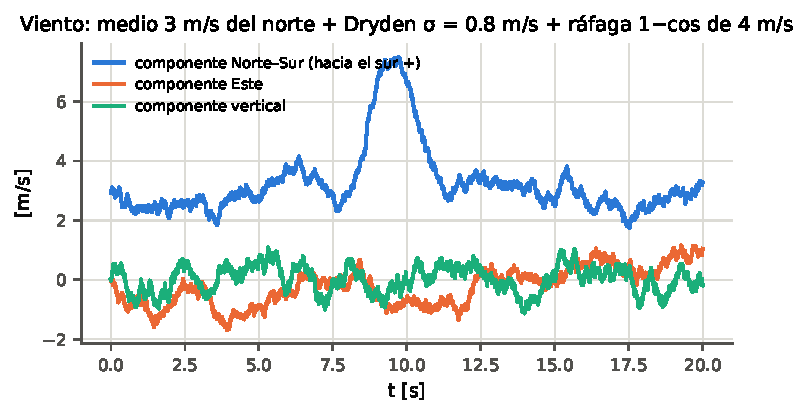
\includegraphics[width=0.85\textwidth]{viento_dryden.pdf}
\caption{Viento medio de 3~m/s del norte, turbulencia de Dryden con
$\sigma=0.8$~m/s y ráfaga $1-\cos$ de 4~m/s entre 8 y 11~s.}
\label{fig:viento}
\end{figure}

\subsection{Interferencia electromagnética en el magnetómetro}

Las corrientes de los ESC y del cableado de potencia generan un campo que
se suma al terrestre en el magnetómetro. El modelo
(\cod{DisturbanceManager.\_emi}) lo hace proporcional a una corriente
equivalente:
\begin{equation}
\vect b_{EMI}=k_I\left(\frac14\sum_i\sigma_i^{1.5}\right)\hat{\vect d}_{EMI}+\text{pulsos},
\label{eq:emi}
\end{equation}
con $k_I=15~\mu$T (campo con los cuatro motores a fondo),
$\hat{\vect d}_{EMI}=(0.6,0.8,0)$ en el cuerpo y pulsos opcionales de
amplitud uniforme en $\pm30~\mu$T a una tasa dada (por ejemplo, un servo).
En hover ($\sigma_h=\val{sigmah}$) el campo parásito es \val{emiH}~$\mu$T, el
\val{emiRel}~\% de la componente horizontal del campo terrestre; si el
estimador confiara solo en el magnetómetro, el rumbo se desviaría
\val{emiPsi}$^\circ$. Es la razón por la que PX4 ofrece compensación del
magnetómetro por corriente (\cod{CAL\_MAG\_COMP}). La perturbación afecta
solo a la medida.

\begin{supuesto}[El exponente 1.5]
El comentario del código justifica $\sigma^{1.5}$ como ``potencia de la
hélice $\propto\Omega^3$''. Esa equivalencia vale si el empuje fuera
proporcional al acelerador ($\Omega\propto\sqrt\sigma$), pero en el modelo de
propulsor de este simulador $\Omega$ es afín en $\sigma$
(\cref{eq:esc}); con él, la corriente de fase sería $\propto\Omega^2$ y la de
batería $\propto\Omega^3$. El exponente es por tanto una forma funcional
supuesta, no derivada; como $k_I$ es un parámetro libre de la
perturbación, la discrepancia solo cambia cómo crece la interferencia con el
acelerador.
\end{supuesto}

\subsection{Cambio de masa y carga útil}

Un evento a un tiempo $t$ engancha (o suelta) una masa puntual $m_p$ en la
posición $\vect r$ del cuerpo (\cod{vehicles.with\_payload}). La carga cambia
tres cosas, y las tres le importan al control:
\begin{gather}
m'=m+m_p,\qquad \vect c'=\frac{m\,\vect c+m_p\,\vect r}{m'},\qquad
\vect d_0=\vect c-\vect c',\qquad \vect d=\vect r-\vect c',\label{eq:carga}\\
J'_{xx}=J_{xx}+m(d_{0,y}^2+d_{0,z}^2)+m_p(d_y^2+d_z^2)\quad\text{(y análogos, teorema de Steiner)},\nonumber
\end{gather}
donde $\vect c$ es el centro de masa actual medido en el marco geométrico del
bastidor (cero en el vehículo nominal, distinto de cero si ya había cargas)
y $\vect r$ la posición de la nueva carga en ese mismo marco. Así varias
cargas sucesivas se componen correctamente: cada una traslada el tensor
acumulado al nuevo centro de masa común. Los brazos de palanca de los rotores pasan a medirse desde el nuevo
centro de masa, $(x_i-c'_x,\ y_i-c'_y)$. Solo se conserva la diagonal del
tensor: los productos de inercia que introduce una carga descentrada se
desprecian. El controlador y el mezclador \emph{no se enteran}: siguen
usando el vehículo nominal, que es lo que pasa en un dron real al que se le
cuelga algo.

\begin{table}[H]
\centering
\small
\caption{Efecto de una carga de 300~g en el PAE-X450 (bloque K).}
\label{tab:carga}
\begin{tabularx}{\textwidth}{lXX}
\toprule
& Carga en $(0,0,5)$~cm (debajo) & Carga en $(5,0,0)$~cm (adelante) \\
\midrule
$J_{xx},J_{yy},J_{zz}$ [kg·m$^2$] & \val{plJz} & \val{plJx} \\
Desplazamiento del centro de masa & \val{plCMz}~mm en $z$ & 8.82~mm en $x$ \\
Momento en hover con aceleradores iguales & 0 & \val{plMy}~N·m (morro abajo) \\
Momento normalizado que debe aportar el integrador & 0 & \val{plU} \\
Acelerador de hover & \val{plSig} & \val{plSig} \\
\bottomrule
\end{tabularx}
\end{table}

La carga descentrada produce un momento constante que solo un término
integral puede compensar; la centrada solo cambia la masa y la inercia,
es decir, la ganancia de la planta. Por eso el escenario de carga de los
bancos de comparación (300~g en $(4,4,5)$~cm, enganchada en $t=8$~s) mide a
la vez robustez a la ganancia y rechazo de perturbación.

\subsection{Pérdida de eficiencia de un motor}

A partir de un instante dado, la velocidad de régimen del motor $i$ se
multiplica por $\eta_i<1$ en \eqref{eq:rotor}. Con $\eta=0.8$ el rotor da el
64~\% del empuje para el mismo acelerador. El controlador lo ve como una
perturbación de momento y de empuje que debe absorber con su integrador.

\subsection{Escenarios estándar}

Para que todos los experimentos sean comparables, \cod{scenarios.py} define
cuatro escenarios con nombre: \emph{nominal}; \emph{viento} (3~m/s del
norte, Dryden $\sigma=1$~m/s, ráfaga de 4~m/s del este en $t=6$~s durante
2~s); \emph{carga} (300~g descentrada en $t=8$~s); y \emph{EMI} (15~$\mu$T a
plena potencia más pulsos de 30~$\mu$T a 0.5~Hz).

\section{Integración numérica y tasas de ejecución}
\label{sec:integracion}

¿A qué frecuencia corre realmente la simulación? La pregunta surge porque la
GUI anterior se refrescaba a 50~Hz. La respuesta corta: 50~Hz es la tasa a
la que se \emph{dibuja}; la física avanza a 1~kHz con Runge--Kutta de cuarto
orden. Esta sección explica la arquitectura de relojes, justifica el
integrador y el paso, y presenta la evidencia numérica.

\subsection{Cuatro relojes, como en un autopiloto}

\begin{table}[H]
\centering
\small
\caption{Tasas de ejecución (\cod{SimConfig} y \cod{Simulation.step\_control}).}
\label{tab:tasas}
\begin{tabularx}{\textwidth}{lcX}
\toprule
Reloj & Tasa & Qué se ejecuta \\
\midrule
Física & \val{physHz}~Hz & RK4 sobre el modelo de 17 estados; \val{nsub} subpasos por periodo de control con los aceleradores retenidos (ZOH); renormalización del cuaternión; fase de los rotores; contacto con el suelo \\
Control & \val{ctrlHz}~Hz & perturbaciones, muestreo de sensores, pasa-bajos del acelerómetro y AHRS, filtros del giroscopio, filtro de navegación, lazo de actitud/tasa y mezclador. Es la tasa de \cod{TaskControlFast} del firmware ESP32 \\
Externo & \val{outerHz}~Hz & lazo vertical (modo actitud) o controlador de posición/trayectoria (modo trayectoria), uno de cada \val{nouter} periodos de control \\
Sensores lentos & 100 / 40 / 100~Hz & magnetómetro, barómetro, posición externa; mantienen el último valor entre muestras \\
Registro y GUI & 100~Hz / 50~Hz & solo lectura del estado; no afectan la simulación \\
\bottomrule
\end{tabularx}
\end{table}

La separación de un orden de magnitud entre el lazo de actitud y el de
posición es la que piden Powers, Mellinger y Kumar \cite{hb16} (pp.~317 y
321). En cada periodo de control el orden de las operaciones es: (1)
perturbaciones; (2) sensores, a partir del estado $\vect x_k$ y de su
derivada con los aceleradores del periodo anterior; (3) estimación y
filtros; (4) lazo externo, si toca; (5) lazo de actitud y mezclador, que
fijan $\sigma_k$; (6) dos pasos RK4 de 1~ms con $\sigma_k$ constante.

El paso de física es siempre un submúltiplo exacto del periodo de control,
$\Delta t_{fis}=\Delta t_{ctrl}/n_{sub}$ con $n_{sub}=\operatorname{round}(f_{fis}/f_{ctrl})$.
Si la razón pedida no es entera, la tasa de física efectiva difiere un poco
de la pedida, pero el reloj y la integración siguen sincronizados. Antes se
integraban $n_{sub}$ pasos de $1/f_{fis}$ mientras el reloj avanzaba
$1/f_{ctrl}$: con 400~Hz de control una caída libre salía un 20~\% lenta y
con 2000~Hz, el doble de rápida, y \cod{ctrl\_hz} es un parámetro que los
barridos pueden variar.

\begin{nota}[Retardo de cómputo, ESC y resolución del acelerador]
Por defecto el mando $\sigma_k$ calculado con las medidas de $t_k$ se aplica
desde $t_k$, sin el periodo de retardo de cómputo que tiene un autopiloto
real (que calcula durante el periodo y aplica al siguiente), y el ESC sigue a
$\sigma$ de forma instantánea y continua, sin frecuencia de PWM ni
protocolo. La cadena de medida sí tiene sus retardos (IMU 2~ms, más el filtro
y la retención).

La edición anterior despachaba la omisión como ``2~ms frente a los 16~ms de
retardo equivalente''. Esa comparación usa el retardo agregado de SIMC y
subestima el efecto, porque lo que importa es la fase en la frecuencia de
cruce. El guion \cod{experiments/delay\_margins.py} lo mide para el lazo de
tasa de roll con las ganancias por defecto, de dos maneras: margen de fase y
multiplicador máximo de las ganancias del lazo lineal en hover, y una
bisección en la simulación 6-DOF completa hasta que aparece una oscilación
sostenida. La \cref{tab:margenes} resume los casos. Un periodo de cómputo
quita 3.3$^\circ$ de margen de fase y baja la ganancia admisible de 5.4 a
4.3 veces; un ESC con PWM estándar de 50~Hz la deja en 2.4 veces. El motor
pesa todavía más: según la revisión externa, con $T_m=30$~ms en lugar de 20
el margen baja a 48$^\circ$. Un barrido que explore ganancias de tasa hasta
2.5 veces el valor SIMC puede encontrar, en simulación, una sintonía que en
el dron oscile.

Para estudiarlo, \cod{SimConfig} ofrece cuatro opciones desactivadas por
defecto: \cod{compute\_delay\_samples} (aplica $\sigma_{k-n}$ en lugar de
$\sigma_k$), \cod{esc\_rate\_hz} (muestreo y retención del mando a la tasa
del ESC), \cod{esc\_pulse\_delay\_s} (el valor retenido actúa un ancho de
pulso después) y \cod{throttle\_levels} (cuantiza $\sigma$ a un número finito
de niveles, como el LEDC del ESP32). Los valores por defecto conservan el
comportamiento con el que se identificaron los rezagos y se afinaron los
controladores de este documento, y así seguirán hasta tener los datos reales
del ESC y del firmware del dron (\cref{sec:limitaciones}).
\end{nota}

\begin{table}[H]
\centering
\small
\caption{Margen del lazo de tasa de roll del PAE-X450 con las ganancias por
defecto y distintas cadenas de actuación
(\cod{experiments/results/delay\_margins/}). Cruce en 4.7~Hz en todos los
casos. Ganancia máxima: factor común sobre $K_p$, $K_i$ y $K_d$ de tasa antes
de la inestabilidad, en el lazo lineal y en la simulación completa. Las
filas son escenarios, no mediciones del dron.}
\label{tab:margenes}
\begin{tabular}{lcccc}
\toprule
Cadena de actuación & MF [$^\circ$] & MG [dB] & Gan. máx. (lineal) & Gan. máx. (6-DOF) \\
\midrule
Continua, sin cómputo (por defecto) & 58.7 & 14.6 & 5.39 & 4.91 \\
+1 periodo de cómputo (2~ms) & 55.4 & 12.7 & 4.30 & 3.91 \\
+2 periodos de cómputo (4~ms) & 52.0 & 11.1 & 3.60 & 3.22 \\
ESC 400~Hz + 1 periodo & 53.2 & 11.7 & 3.84 & 3.67 \\
ESC 400~Hz + 1 periodo + pulso 1.5~ms & 50.7 & 10.6 & 3.40 & 3.22 \\
ESC 50~Hz + pulso 1.5~ms & 39.6 & 7.8 & 2.44 & 2.25 \\
\bottomrule
\end{tabular}
\end{table}

\subsection{Los integradores}

Con la entrada constante en el paso, $\dot{\vect x}=f(\vect x)$, el código
(\cod{dynamics.rk4\_step}) implementa Runge--Kutta clásico:
\begin{equation}
\begin{gathered}
\vect k_1=f(\vect x_n),\quad
\vect k_2=f\!\big(\vect x_n+\tfrac{h}{2}\vect k_1\big),\quad
\vect k_3=f\!\big(\vect x_n+\tfrac{h}{2}\vect k_2\big),\quad
\vect k_4=f(\vect x_n+h\vect k_3),\\
\vect x_{n+1}=\vect x_n+\tfrac{h}{6}\big(\vect k_1+2\vect k_2+2\vect k_3+\vect k_4\big),
\end{gathered}
\label{eq:rk4}
\end{equation}
con error local $O(h^5)$ y global $O(h^4)$ \cite{hairer93}. Euler explícito,
$\vect x_{n+1}=\vect x_n+h f(\vect x_n)$ (global $O(h)$), se conserva solo
para comparar (\cod{SimConfig.integrator="euler"}).

\paragraph{Estabilidad.} El modo más rápido del modelo en lazo abierto es el
del motor, $\lambda=-1/T_m=-50$~s$^{-1}$ (\cref{tab:jac}). A 1~kHz,
$h\lambda=-0.05$. Euler es estable para $h\lambda\in(-2,0)$, o sea
$h<2T_m=40$~ms; RK4, en el eje real, para $h\lambda>-2.785$, o sea
$h<55.7$~ms. La estabilidad numérica no es la restricción que fija el paso:
lo son la exactitud y la necesidad de que la física sea más rápida que el
lazo de control que la observa. El NMPC de la \cref{sec:posicion}, con paso de
predicción de 50~ms, sí queda cerca de ese límite en su modelo interno
($\Delta t_{pred}/\tau_T=2.6$), y por eso integra exactamente sus estados de
rezago.

\paragraph{La vibración no necesita física más rápida.} El tono de 177~Hz
podría parecer un argumento para integrar más rápido. No lo es: la fase de
cada rotor se avanza analíticamente, $\varphi_i\leftarrow\varphi_i+\Omega_i h$,
y el sensor la evalúa en los instantes de muestreo. El tono que ve la IMU es
exacto para cualquier paso de física.

\subsection{Evidencia numérica}

\paragraph{Orden de convergencia.} El bloque E integra durante 1~s una
maniobra no lineal genérica (velocidad de $(3,-2,1)$~m/s, actitud y velocidad
angular no nulas, rotores desbalanceados, aceleradores fijos distintos) con
pasos de 8~ms a 0.25~ms, y compara con una solución de referencia RK4 de
$h=25~\mu$s. Se comprobó que a lo largo de la referencia ninguna componente
de $\vect v_B$ ni de $\vect\omega$ cruza cero (mínimo $|\cdot|$ =
\val{minVb}): las funciones $x|x|$ del arrastre no tienen ``esquinas'' en el
intervalo, condición para que RK4 alcance su orden.

\begin{figure}[H]
\centering
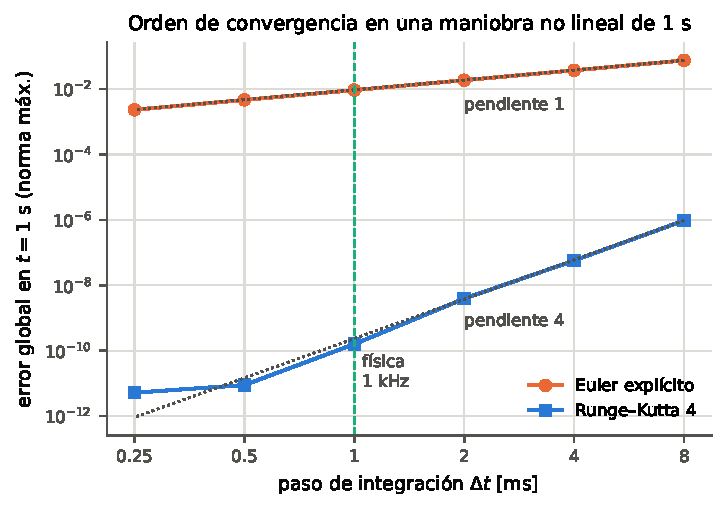
\includegraphics[width=0.72\textwidth]{convergencia_integradores.pdf}
\caption{Error global en $t=1$~s frente al paso. Pendientes ajustadas: Euler
\val{ordEuler}, RK4 \val{ordRK} (pares sucesivos: \val{ordRKpares}). El último
punto de RK4 toca el piso de redondeo ($\approx$\val{errRKfloor}).}
\label{fig:conv}
\end{figure}

Las pendientes medidas, \val{ordEuler} y \val{ordRK}, son las teóricas 1 y 4.
Al paso de 1~ms el error de RK4 es \val{errRK1ms}; un Euler explícito con el paso
de 2~ms de la 2.ª edición tiene \val{errEu2ms}, ocho órdenes de magnitud más.

\paragraph{Conservación en rotación libre.} Sin arrastre, sin
amortiguamiento y con los rotores parados, el cuerpo rígido conserva la
energía $E=\tfrac12\vect\omega\T J\vect\omega$ y el momento angular en el
marco inercial, $\vect L_E=\R J\vect\omega$. Son invariantes exactos que
ningún integrador de paso fijo genérico conserva por construcción; medir su
deriva es una prueba independiente. Además, el PAE-X450 cumple
$J_{yy}<J_{xx}<J_{zz}$, así que un giro alrededor de $x$ es un giro
alrededor del eje \emph{intermedio}, inestable (efecto Dzhanibekov o
teorema de la raqueta de tenis \cite{landau76}). Linealizando las
ecuaciones de Euler alrededor de $\vect\omega=(\omega_0,0,0)$, las
perturbaciones crecen con tasa
\begin{equation}
\lambda=\omega_0\sqrt{\frac{(J_{xx}-J_{yy})(J_{zz}-J_{xx})}{J_{yy}J_{zz}}}=\val{dzLam}~\text{s}^{-1}\quad(\omega_0=20~\text{rad/s}).
\label{eq:dzh}
\end{equation}
Con perturbaciones iniciales de $10^{-3}$~rad/s, la primera inversión se
espera hacia $\ln(20/1.4\times10^{-3})/\lambda\approx\val{dzEst}$~s; la
simulación la da a los \val{dzFirst}~s y muestra \val{dzFlips} inversiones de
$\omega_x$ en 40~s (\cref{fig:dzh}). Los ejes estables sí lo son: girando
alrededor de $z$ (inercia máxima) o de $y$ (mínima), las componentes
transversales se quedan por debajo de \val{stabZ} y \val{stabY}~rad/s en
10~s.

\begin{figure}[H]
\centering
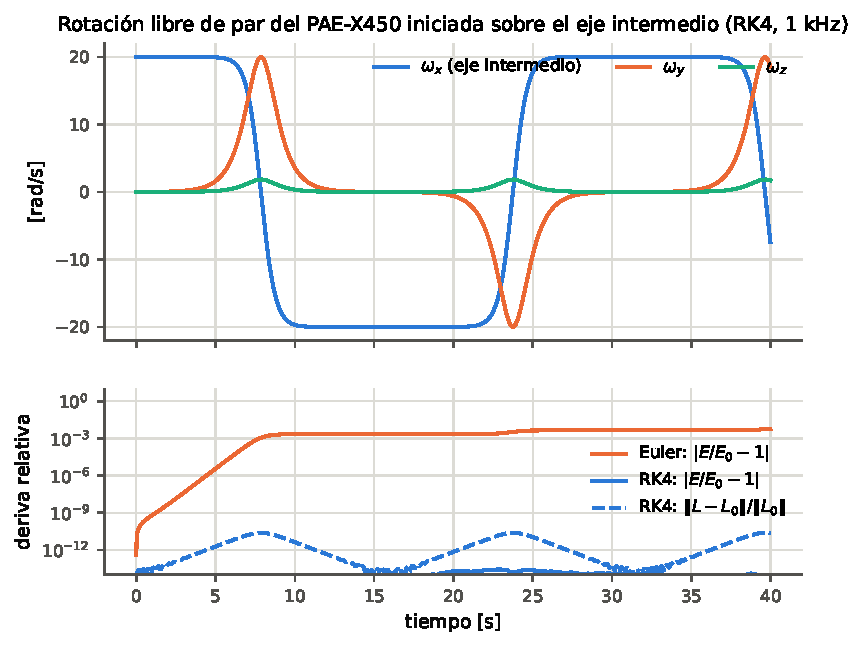
\includegraphics[width=0.8\textwidth]{dzhanibekov_conservacion.pdf}
\caption{Rotación libre iniciada sobre el eje intermedio. Arriba: inversiones
periódicas de $\omega_x$. Abajo: deriva relativa de la energía y del momento
angular inercial con RK4 y con Euler a 1~kHz.}
\label{fig:dzh}
\end{figure}

Con RK4 a 1~kHz la deriva máxima en 40~s es \val{freeRKE} en energía y
\val{freeRKL} en momento angular; con Euler al mismo paso, \val{freeEuE} y
\val{freeEuL}. La diferencia muestra qué tan engañoso puede ser Euler en una
simulación larga: inyecta energía, y lo hace justo en las fases rápidas de la
inversión.

\paragraph{Exactitud en lazo cerrado.} La prueba que más le importa al
usuario es si la frecuencia de física cambia los resultados del simulador
completo. El bloque E corre 3~s con escalones de roll de $\pm15^\circ$
(estimador ideal, sensores sin ruido, controlador a 500~Hz) con física a
16~kHz como referencia y compara:

\begin{table}[H]
\centering
\small
\caption{Error máximo frente a la referencia de 16~kHz en lazo cerrado.}
\label{tab:cl}
\begin{tabular}{lcc}
\toprule
Integrador y tasa de física & roll [$^\circ$] & posición lateral $y$ [m] \\
\midrule
RK4, 1000~Hz (por defecto) & \val{clRKmilphi} & \val{clRKmily} \\
RK4, 500~Hz & \val{clRKquiphi} & \val{clRKquiy} \\
Euler, 1000~Hz & \val{clEumilphi} & \val{clEumily} \\
Euler, 500~Hz (2.ª edición) & \val{clEuquiphi} & \val{clEuquiy} \\
\bottomrule
\end{tabular}
\end{table}

Con RK4 la física a 1~kHz es indistinguible de la de 16~kHz (error de
millonésimas de grado) y la de 500~Hz también bastaría; los 1000~Hz se
eligieron por margen, a un costo bajo. Euler a 500~Hz se separa
\val{clEuquiphi}$^\circ$ en roll y \val{clEuquiy}~m en posición lateral en
tres segundos: no es catastrófico, pero es del orden
de los efectos que se quieren estudiar (errores de estimación de décimas de
grado, errores de seguimiento de centímetros), y crece con la duración.

\paragraph{Costo.} Con el estimador por defecto (\val{estDef}), el simulador
completo corre a unas \val{rtf} veces el tiempo real en un núcleo (bloque L;
medido con otro proceso pesado compartiendo la CPU), suficiente para
barridos de cientos de corridas y para la GUI en tiempo real.

\section{Controladores de posición y trayectoria}
\label{sec:posicion}

Una decisión de diseño del proyecto fue conservar la cascada PID de bajo
nivel, que es suficiente para la actitud, y comparar las técnicas avanzadas
\emph{encima} de ella, en el lazo de posición. El simulador tiene cinco controladores con una interfaz común, siete
generadores de trayectoria, un procedimiento de identificación de los
rezagos que los controladores basados en modelo necesitan y un banco de
comparación con métricas sobre la posición verdadera.

\subsection{Interfaz común y restricciones compartidas}

Todos los controladores heredan \cod{PositionController} y corren en el lazo
externo (100~Hz):
\begin{equation}
\texttt{update}(t,\ \text{NavState},\ \text{trayectoria})\ \to\ (\vect a_{des},\ \psi_{ref},\ \dot\psi_{ff})\ \ [\text{u opcionalmente } (T,\phi,\theta,\psi)].
\end{equation}
\cod{NavState} contiene solo cantidades \emph{estimadas} (posición y
velocidad del filtro de navegación, actitud del AHRS, tasas filtradas y la
aceleración cinemática estimada $\vect a_{kin,E}$ de \eqref{eq:akin}) y la
masa \emph{nominal}: el controlador no sabe si alguien le colgó una carga.
La aceleración deseada pasa por la planitud diferencial de la
\cref{sec:planitud}; solo el NMPC entrega empuje y actitud directamente.

Para que la comparación sea justa, PID, MPC y NMPC comparten la misma caja de
aceleraciones admisibles (\cod{common.accel\_limits}):
\begin{equation}
|a_x|,|a_y|\le g\tan30^\circ=\val{axyMax}~\text{m/s}^2,\qquad
-0.8\Big(\frac{T_{max}}{m}-g\Big)=-\val{aUp}\ \le a_z\le\ 0.8\,g=\val{aDown}~\text{m/s}^2 .
\label{eq:caja}
\end{equation}
El factor 0.8 deja un 20~\% de empuje al lazo de actitud: los motores no
pueden dar a la vez todo el empuje y todo el momento (\cref{sec:propulsion}).
El PID acota la norma horizontal en lugar de cada eje, y la política de RL
proyecta sobre un cono de $30^\circ$ con $a_z\in[-6,6]$~m/s$^2$; las tres
formas coinciden en la inclinación máxima en hover sostenido.

\subsection{Generadores de trayectoria}

Cada trayectoria (\cod{trajectories.py}) entrega la referencia y sus tres
primeras derivadas \emph{analíticas}, $(\vect p,\vect v,\vect a,\vect j)$,
más el rumbo. Los controladores las usan como prealimentación y el MPC y el
NMPC como previsión del horizonte. Hay siete: vuelo estacionario,
escalones (caja en XY más escalón de altura), círculo, figura en 8, hélice,
mínimo \emph{snap} por puntos de paso y punto a punto de mínimo
\emph{jerk}.

\paragraph{Arranque desde el reposo.} Una curva periódica pura, por ejemplo
$x=R\cos\omega t$, arranca con velocidad $R\omega$: un escalón en la
referencia de velocidad que ningún dron puede seguir y que contaminaría las
métricas con un transitorio arbitrario. Las curvas periódicas se recorren
con una fase $\vartheta(t)$ cuya velocidad sube con el polinomio
\emph{smoothstep} de quinto orden,
\begin{equation}
\dot\vartheta=\omega\,s\!\left(\frac{t}{T_r}\right),\qquad s(u)=10u^3-15u^4+6u^5,
\label{eq:smooth}
\end{equation}
que cumple $s(0)=0$, $s(1)=1$ y $s'=s''=0$ en ambos extremos. Por la regla
de la cadena,
\begin{equation}
\vect v=\vect f'\dot\vartheta,\quad
\vect a=\vect f''\dot\vartheta^2+\vect f'\ddot\vartheta,\quad
\vect j=\vect f'''\dot\vartheta^3+3\vect f''\dot\vartheta\ddot\vartheta+\vect f'\dddot\vartheta,
\end{equation}
y en $t=0$ velocidad, aceleración y \emph{jerk} son exactamente cero (el
bloque M lo verifica: $\max|\cdot|=0$). Como $\int_0^1s=1/2$, la rampa recorre
media vuelta equivalente; con la rampa simétrica de bajada la trayectoria
termina en reposo en el punto de partida tras un número entero de vueltas,
y dura $n_{vueltas}T+T_r$.

\paragraph{Figura en 8.} Lemniscata de Gerono en el plano horizontal,
\begin{equation}
x=c_x+A\sin\vartheta,\qquad y=c_y+\tfrac{B}{2}\sin2\vartheta,
\label{eq:gerono}
\end{equation}
con $A=2$~m y $B=1$~m (el 8 mide $4\times1$~m). Es la prueba clásica de
seguimiento en la literatura de MPC para cuadricópteros
\cite{torrente21,sun22}, aunque esos trabajos la usan a velocidades mucho
mayores y con otra parametrización; la de Gerono se eligió por su forma
cerrada. Con periodo de 10~s (dos vueltas) alcanza \val{lemV}~m/s y
\val{lemA}~m/s$^2$ (inclinación de \val{lemTilt}$^\circ$); la versión rápida
del banco, con periodo de 5~s y tres vueltas, \val{lemRV}~m/s y
\val{lemRA}~m/s$^2$, que exigen \val{lemRTilt}$^\circ$ de inclinación, cerca del
límite de 30$^\circ$. El círculo de 1.5~m y 10~s llega a \val{cirV}~m/s.

\paragraph{Mínimo snap.} Para recorrer puntos de paso, Mellinger y Kumar
\cite{mellinger11} minimizan $\int\|\vect p^{(4)}\|^2dt$. Por
Euler--Lagrange la solución cumple $\vect p^{(8)}=0$ en cada tramo:
polinomios de grado 7. Con la asignación de tiempos fija
($T_i=\max(t_{min},d_i/\bar v)$), posiciones impuestas en los puntos de
paso, reposo ($v=a=j=0$) en los extremos y continuidad de las derivadas 1 a
6 en los puntos interiores, el número de ecuaciones iguala al de incógnitas
($8M$ para $M$ tramos) y la solución del sistema lineal \emph{es} el mínimo
\cite{richter13}. Cada tramo usa tiempo normalizado $\tau\in[0,1]$ para que
la matriz esté bien condicionada. Verificación: el salto relativo de las
derivadas 1--6 en los nudos es \val{msJump}.

\subsection{Identificación de los rezagos del lazo interno}
\label{sec:identificacion}

Visto desde el lazo de posición, todo lo que hay debajo (planitud, AHRS,
cascada de actitud, mezclador, motores) es un sistema
$\vect a_{des}\to\vect a$. Los controladores basados en modelo necesitan
una descripción simple de él. \cod{identification.py} la obtiene con un
ensayo de escalón sobre el simulador \emph{completo}, como en un banco
real: el dron arranca en hover, un comandante en lazo abierto aplica un
escalón $+U$ y, en otra corrida con la misma semilla, $-U$; la semidiferencia
cancela la deriva común (sesgos, ruido). Sobre esa respuesta se ajusta por
mínimos cuadrados
\begin{equation}
y(t)=K\,U\left(1-e^{-(t-\theta)/\tau}\right),\quad t>\theta,
\label{eq:fopdt}
\end{equation}
con búsqueda en malla sobre $(\theta,\tau)$ y $K$ lineal en cada punto, en
dos versiones: primer orden con retardo (FOPDT) y primer orden puro
($\theta=0$, que absorbe el retardo en $\tau$ por la regla de la mitad).

\begin{table}[H]
\centering
\small
\caption{Rezagos identificados del PAE-X450 que usan los controladores
(\cod{DEFAULT\_LAGS}; identificados con Madgwick y el núcleo anterior,
escalones de 1.5~m/s$^2$ y $8^\circ$). Error RMS relativo del ajuste entre
paréntesis.}
\label{tab:lags}
\begin{tabular}{lcc}
\toprule
Canal & Primer orden puro & FOPDT \\
\midrule
$a_{des,xy}\to a_{xy}$ & $\tau_{a,xy}=\val{tauAxy}$~ms (\val{rmseFO}~\%) & $\val{tauAxyF}$~ms $+$ \val{thAxyF}~ms (\val{rmseFOPDT}~\%) \\
$a_{des,z}\to a_z$ & $\tau_{a,z}=\val{tauAz}$~ms (\val{rmseZ}~\%) & igual, sin retardo \\
$\phi_{ref}\to\phi$ & $\tau_{att}=\val{tauAtt}$~ms & $\val{tauAttF}$~ms $+$ \val{thAttF}~ms \\
\bottomrule
\end{tabular}
\end{table}

\begin{figure}[H]
\centering
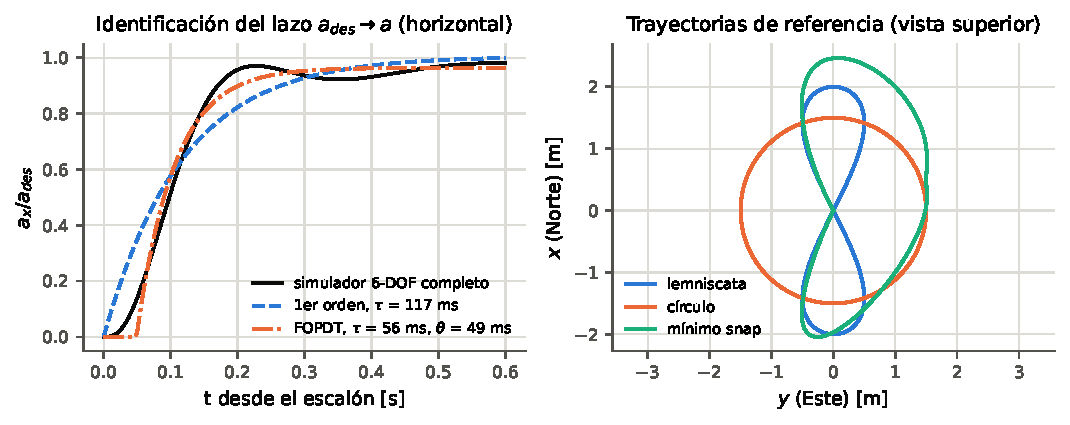
\includegraphics[width=\textwidth]{identificacion_trayectorias.pdf}
\caption{Izquierda: respuesta del simulador completo a un escalón de
aceleración horizontal y los dos ajustes. Derecha: figura en 8, círculo y
trayectoria de mínimo snap por defecto (vista superior).}
\label{fig:ident}
\end{figure}

La lectura de la \cref{fig:ident} es importante para entender los resultados
del banco. El lazo horizontal no es de primer orden: es de segundo orden,
con una curva en S, una joroba hacia los 0.2~s y una cola lenta que deja el
integrador del lazo de tasa. El primer orden puro de 119~ms comete un 7.5~\%
de error; el FOPDT, 3.1~\%. El canal vertical, en cambio, es casi
exactamente el motor ($T_m=20$~ms). Todos los controladores basados en
modelo comparten ese error de modelado.

La \cref{tab:lags} es la que usan los controladores, y se identificó con el
núcleo anterior. El ensayo de la \cref{fig:ident} se repitió con el núcleo
actual (estimador \val{estDef}, acelerómetro filtrado, $k_d=K_c\theta$,
giroscopio a 60~Hz; bloque M): el canal horizontal da
$\tau=\val{reidTau}$~ms como primer orden puro (\val{reidRmseFO}~\% de error)
y $\val{reidTauF}~\text{ms}+\val{reidThF}~\text{ms}$ como FOPDT
(\val{reidRmseFOPDT}~\%). \cod{DEFAULT\_LAGS} no se regeneró tras el cambio
del núcleo.

\subsection{PID en cascada (estilo PX4)}

\cod{position/pid.py} reproduce la estructura de \cod{mc\_pos\_control} de
PX4: un P de posición que genera una referencia de velocidad, y un PID de
velocidad con prealimentación de la velocidad y la aceleración de
referencia:
\begin{align}
\vect v_{sp}&=\vect v_{ref}+\sat_{v_{max}}\!\big(K_p(\vect p_{ref}-\hat{\vect p})\big),\qquad
\vect e_v=\vect v_{sp}-\hat{\vect v},\nonumber\\
\vect a_{des}&=\sat_{\text{caja}}\Big(\vect a_{ref}+K_v\vect e_v+K_i\!\int\!\vect e_v\,dt+K_d\,\tfrac{d}{dt}\vect e_v\Big),
\label{eq:pidpos}
\end{align}
con la corrección de velocidad acotada ($3$~m/s en XY, $2$~m/s en $z$),
integración condicional e integral acotada como en \eqref{eq:pid}, y el
derivativo filtrado a 5~Hz (apagado por defecto, $K_d=0$). Sin
prealimentación un lazo de posición solo corrige \emph{después} de que el
error aparece.

\paragraph{Ganancias derivadas del modelo.} Con las mismas reglas SIMC de
la \cref{sec:control} sobre la planta identificada: el lazo de velocidad ve
$a_{cmd}\to v=1/s$ con el FOPDT de la \cref{tab:lags}, y la regla de la mitad
da $\theta_{ef}=\tau+\theta+\Delta t/2$ ($\Delta t/2$ es la retención del lazo
de 100~Hz). Con $\tau_c=\max(1.5\,\theta_{ef},\,0.1~\text{s})$, más
conservador que el ``ajustado'' $\tau_c=\theta$ para dejar margen al ruido del
estimador,
\begin{equation}
K_v=\frac{1}{\tau_c+\theta_{ef}},\quad K_i=\frac{K_v}{4(\tau_c+\theta_{ef})},\quad
K_p=\frac{1}{3\,(\tau_c+\theta_{ef})}.
\end{equation}
Resulta $K_p=\val{pdkpxy}$, $K_v=\val{pdkvxy}$, $K_i=\val{pdkixy}$ en XY y
$K_p=\val{pdkpz}$, $K_v=\val{pdkvz}$, $K_i=\val{pdkiz}$ en $z$; los valores por
defecto de PX4 son todavía más conservadores (0.95 / 1.8 / 0.4 en XY).

\paragraph{Ganancias afinadas en simulación.} Para el PAE-X450, $K_p$ y $K_v$
salen de una malla $K_p\in\{2.4,3,3.6,4.5\}\times K_v\in\{4.5,5.5,6.5\}$ con
$K_i=K_v^2/4$ (la relación SIMC $T_i=4/K_v$), escogiendo el mínimo del RMSE
medio en figura en 8 y círculo: $K_p=3.6$, $K_v=5.5$, $K_i=7.56$, que bajó el
RMSE de 6.2 a 3.1~cm frente a las ganancias derivadas (malla hecha con el
núcleo anterior y Madgwick, escenario nominal, semilla 1). El MPC y el NMPC
se afinaron con el mismo protocolo. Esa semilla es también una de las tres
del banco final, y el integral se eligió mirando el caso con interferencia
magnética (nota siguiente): los tres controladores clásicos se afinaron
sobre parte del conjunto de prueba, cosa que no se hizo con el RL
(\cref{sec:banco}). Es, en pequeño, el flujo que propone el proyecto: sintonía en
simulación como punto de partida. El valor por defecto actual del integral
es, sin embargo, $K_{i,xy}=\val{pidKiDef}$, por la razón de la nota
siguiente: el óptimo en el escenario nominal no es el óptimo robusto.

\begin{nota}[Fragilidad del integral con interferencia magnética]
Las cifras de esta nota son anteriores a restringir la corrección magnética
al rumbo (\cref{sec:estimadores}); el banco final de la \cref{sec:banco} ya
incluye ese cambio. Con EMI en el magnetómetro el rumbo estimado se desviaba 11--12$^\circ$; el
empuje real queda rotado respecto de la aceleración pedida, y un integral
grande sobre una planta rotada entra en espiral. Con el núcleo actual
(Mahony, acelerómetro filtrado), en la figura en 8 nominal $K_{i,xy}=2$ dio
2.35~cm de RMSE frente a 2.38~cm con 7.56; con EMI, 4.99~cm frente a 73~cm
(semilla 1, medido antes de corregir el desfase de 10~ms del registro de la
referencia que se explica en la \cref{sec:banco}; el orden de magnitud de la
diferencia no depende de esa corrección).
Por eso el valor por defecto pasó a 2.0. Aun así, con EMI y
\emph{escalones} de 1~m el PID entra en un ciclo límite saturado en la
inclinación máxima: es un hallazgo del banco, no un error de
implementación. El MPC, cuyo observador de perturbación estima la
aceleración no explicada en lugar de integrar el error, no lo sufre.
\end{nota}

\subsection{MPC lineal con previsión}

\paragraph{Modelo de predicción.} Por eje, desacoplado, con la aceleración
total como estado y el rezago identificado (\cod{position/mpc.py}):
\begin{equation}
\dot p=v,\qquad \dot v=a,\qquad \dot a=\frac{u-a}{\tau_a},\qquad
\vect x=[p,v,a]\T,\ u=a_{cmd},
\label{eq:mpc_model}
\end{equation}
con $\tau_a=\tau_{a,xy}$ en $x,y$ y $\tau_{a,z}$ en $z$. Se discretiza de
forma \emph{exacta} con retención de orden cero y paso $h=\Delta t_{pred}$;
con $\alpha=e^{-h/\tau}$ y $\beta=1-\alpha$:
\begin{equation}
A=\begin{bmatrix}1&h&\tau(h-\tau\beta)\\0&1&\tau\beta\\0&0&\alpha\end{bmatrix},\qquad
B=\begin{bmatrix}h^2/2-\tau h+\tau^2\beta\\ h-\tau\beta\\ \beta\end{bmatrix}.
\label{eq:zoh}
\end{equation}
El bloque M compara \eqref{eq:zoh} con la exponencial de la matriz aumentada
(\cod{scipy.linalg.expm}) para tres $\tau$ y dos pasos: error máximo
\val{zohErr}.

\paragraph{Costo.} Sobre un horizonte de $N=20$ pasos de 50~ms (1~s), con la
referencia muestreada en $t+kh$:
\begin{equation}
J=\sum_{k=1}^{N}q_p(p_k-p_{ref,k})^2+q_v(v_k-v_{ref,k})^2
+\sum_{k=0}^{N-1}r_u\,(u_k-u_{ref,k})^2+r_{du}(u_k-u_{k-1})^2 .
\label{eq:mpc_cost}
\end{equation}
La entrada de referencia es la que hace que el modelo con rezago siga
exactamente la aceleración de referencia: si $a=a_{ref}$, entonces
$u_{ref}=a_{ref}+\tau_a\,j_{ref}$, evaluada en el centro de cada intervalo.
Con $u_{ref}=0$ el término $r_uu^2$ sesgaría el seguimiento hacia
aceleración nula (en un círculo, hacia adentro); penalizando la
\emph{desviación} el sesgo desaparece. Pesos por defecto: $q_p=1$, $q_v=0$
en XY; $q_{pz}=2$, $q_{vz}=0.1$; $r_u=5\times10^{-4}$, $r_{du}=0$.

\paragraph{QP condensado y su solución.} Eliminando los estados con
$\vect p=\Phi\vect x_0+\Gamma\vect U$, el costo es una cuadrática en las $N$
entradas, $\tfrac12\vect U\T H\vect U+\vect f\T\vect U$, con
$H=2(q_p\Gamma_p\T\Gamma_p+q_v\Gamma_v\T\Gamma_v+r_uI+r_{du}D\T D)$ precalculada y
$\vect f$ lineal en el estado y en la previsión. Las únicas restricciones son
la caja \eqref{eq:caja} sobre $\vect U$, así que la proyección es exacta y
barata. El algoritmo: (1) se calcula el óptimo sin restricciones
$\vect U^*=-H^{-1}\vect f$; si cumple la caja, es el óptimo exacto (caso más
común en el banco). (2) Si no, FISTA \cite{beck09} con reinicio por
gradiente \cite{odonoghue15}, precondicionado diagonal (Jacobi:
$\tilde H=SHS$, $S=\diag(H)^{-1/2}$), paso $1/L$ con $L=\lambda_{max}(\tilde H)$,
arranque en caliente con la solución anterior desplazada y un máximo de 60
iteraciones. Con ese tope el costo queda a menos del 0.3~\% del óptimo y el
tiempo medio es de 0.4~ms por llamada.

\paragraph{Estado no medido y acción libre de offset.} La aceleración no se
mide: se usa la predicción del modelo interno, la última entrada aplicada
filtrada por el mismo rezago,
$a_{lag}\leftarrow e^{-\Delta t/\tau}a_{lag}+(1-e^{-\Delta t/\tau})u_{apl}$. Para
rechazar perturbaciones constantes (viento medio, carga, error de empuje)
se agrega un observador de Luenberger de perturbación de entrada
(\cod{common.DisturbanceObserver}) sobre el modelo $\dot v=a_{lag}+d$,
$\dot d=0$, con la velocidad estimada como medida:
\begin{equation}
\hat v\leftarrow\hat v+\Delta t\,\big(a_{lag}+\hat d+\ell_1(v-\hat v)\big),\qquad
\hat d\leftarrow\hat d+\Delta t\,\ell_2(v-\hat v),\qquad
s^2+\ell_1s+\ell_2=s^2+2\zeta\omega s+\omega^2,
\label{eq:dob}
\end{equation}
con $\omega=3$~rad/s y $\zeta=0.8$ (polos en $-2.4\pm1.8j$). Es el esquema
``offset-free'' de Pannocchia y Rawlings \cite{pannocchia03} y Maeder,
Borrelli y Morari \cite{maeder09}: $\hat d$ absorbe todo lo que el modelo no
explica. El QP trabaja con la aceleración total $a=a_{lag}+\hat d$ y la
entrada desplazada $\tilde u=u+\hat d$; se aplica
$u=\sat_{\text{caja}}(\tilde u_0-\hat d)$.

\paragraph{Ley equivalente.} Sin restricciones activas el MPC es una ley
lineal en el estado y en la previsión (\cod{lq\_gain}). Para el eje $x$,
$u_0=-\val{mpcKx}\,(p-p_{ref})-\val{mpcKvx}\,v-\val{mpcKax}\,a+(\text{términos de previsión})$;
la suma de las ganancias de posición y de previsión es \val{mpcInv} (debe ser
cero por invarianza a traslaciones). Comparada con el PID afinado (rigidez
$K_pK_v=19.8$~s$^{-2}$, amortiguamiento $K_v=5.5$~s$^{-1}$), el MPC es casi
el doble de rígido y además se anticipa: ve venir la curva un segundo antes.

\subsection{MPC no lineal (iLQR con restricciones de caja)}

\paragraph{Modelo de predicción.} Nueve estados y tres entradas
(\cod{position/nmpc.py}):
\begin{gather}
\vect x=[\vect p,\vect v,\phi,\theta,T],\qquad \vect u=[T_c,\phi_c,\theta_c],\nonumber\\
\dot{\vect p}=\vect v,\quad
\dot{\vect v}=g\eu-\frac{T}{m}\,\vect r_3(\phi,\theta,\psi)-\frac{c_d}{m}\vect v|\vect v|+\hat{\vect d},\quad
\dot\phi=\frac{\phi_c-\phi}{\tau_{att}},\quad
\dot\theta=\frac{\theta_c-\theta}{\tau_{att}},\quad
\dot T=\frac{T_c-T}{\tau_T},
\label{eq:nmpc}
\end{gather}
con $\vect r_3=\R\eu=(c_\phi s_\theta c_\psi+s_\phi s_\psi,\ c_\phi s_\theta s_\psi-s_\phi c_\psi,\ c_\phi c_\theta)$
la tercera columna de la matriz Z-Y-X, $\psi$ el rumbo de referencia
(exógeno), $\tau_{att}=\val{tauAtt}$~ms y $\tau_T=\tau_{a,z}$ de la
\cref{tab:lags}. Es genuinamente no lineal: proyección trigonométrica del
empuje sin aproximar, producto $T\vect r_3$ y arrastre cuadrático (aplicado en
$\E$, supuesto; la planta lo aplica en $\B$, y la diferencia la absorbe
$\hat{\vect d}$).

\paragraph{Discretización.} Los tres estados de rezago son lineales y se
integran exactamente con ZOH; $(\vect p,\vect v)$ con un paso RK4 que evalúa
el rezago en $0,h/2,h$. Un RK4 sobre los nueve estados quedaría al borde de
su región de estabilidad: con $h=50$~ms y $\tau_T=19.5$~ms, $h/\tau_T=2.6$,
cerca del límite de 2.785 en el eje real, y su factor de amplificación por
paso para ese modo sería 0.75 frente al exacto $e^{-2.6}=0.07$.

\paragraph{Costo y referencia.} Cuadrático en el error de posición y
velocidad y en la desviación de las entradas respecto de una referencia
$\vect u_{ref}$ que sale de la planitud diferencial
(\cref{sec:planitud}) aplicada a $\vect a_{ref}+\tau_{att}\vect j_{ref}-\hat{\vect d}+\frac{c_d}{m}\vect v_{ref}|\vect v_{ref}|$,
con peso terminal. Restricciones de caja:
$T_c\in[\val{nmpcTlo},\val{nmpcThi}]$~N (la misma caja vertical del MPC) y
$|\phi_c|,|\theta_c|\le30^\circ$.

\paragraph{Solver.} iLQR \cite{li04,tassa12} con entradas acotadas a la
manera de \emph{box-DDP} \cite{tassa14}. Los jacobianos $A_k,B_k$ se calculan
por diferencias finitas, todos los pasos del horizonte en un solo lote
vectorizado. En el paso hacia atrás, con
$Q_{uu}=\ell_{uu}+B_k\T V_{xx}B_k+\mu I$ y $Q_{ux}=B_k\T V_{xx}A_k$, se
comprueba con Cholesky que $Q_{uu}$ sea definida positiva; si no lo es,
$\mu$ se multiplica por 10 y se repite el paso (regularización adaptativa de
Levenberg--Marquardt, \cite{tassa12}), y tras un paso exitoso vuelve a bajar.
Con jacobianos por diferencias finitas, $V_{xx}$ puede perder la definición
positiva en saturación o ante perturbaciones grandes. Luego se
resuelve en cada $k$ el QP de caja de dimensión 3 para la corrección
$\delta\vect u_k$ por Newton proyectado, y las filas de la ganancia
$K_k=-Q_{uu}^{-1}Q_{ux}$ de las entradas que quedaron en su cota se anulan
(no hay realimentación en una dirección saturada). El paso hacia adelante
simula en lote los candidatos $\alpha\in\{1,0.5,0.25,0\}$,
$\vect u_k=\sat(\vect U_k+\alpha\,\delta\vect u_k+K_k(\hat{\vect x}_k-\vect X_k))$, y
se queda con el de menor costo; $\alpha=0$ es el despliegue en lazo cerrado
del arranque en caliente, así que el costo nunca empeora. Se hace una
iteración por llamada con arranque en caliente (iteración en tiempo real,
\cite{diehl05}); el costo medido en la máquina de desarrollo es de
3.8~ms de mediana por llamada
(\cod{experiments/nmpc\_timing.py}), y depende mucho del procesador y de la
versión de Python y numpy: otra máquina midió 16~ms. Las pruebas de tiempo
de cómputo, por esa razón, no corren por defecto.

\paragraph{Por qué no supera al MPC lineal.} Medido en la figura en 8
rápida (con el núcleo anterior y Madgwick): con 1, 2 o 3 iteraciones el RMSE apenas cambia (5.24, 5.15,
5.20~cm), de modo que el optimizador no es el límite; quitando el arrastre
del modelo tampoco empeora. Hasta unos $16^\circ$ de inclinación la
proyección trigonométrica es casi lineal, y ambos comparten el error de
modelo dominante: el lazo de actitud real es de segundo orden con unos
43~ms de retardo, no un primer orden (\cref{fig:ident}).

\subsection{Aprendizaje por refuerzo puro (PPO fuera de línea)}

El requisito de diseño fue no entrenar nunca un RL sobre una planta lenta:
entrenar fuera de línea en un entorno rápido, después transferir y validar.
El simulador 6-DOF corre a unas 10 veces el tiempo real; PPO necesita del
orden de $10^7$ pasos, que en el 6-DOF serían horas por millón. Por eso el
flujo (detallado en \cod{docs/RL.md}) fue el siguiente. Las políticas se
entrenaron con el núcleo anterior (sustituto identificado con Madgwick) y
\emph{no se reentrenaron} tras las correcciones; en el banco final actúan
sobre el núcleo actual sin cambios, lo que es en sí una prueba adicional de
transferencia.

\begin{enumerate}
\item \textbf{Sustituto identificado.} Solo la traslación, con el lazo
interno como retardo más primer orden por eje y la masa real distinta de
la nominal,
\begin{equation}
\vect a_{thr}=\frac{e^{-d s}}{\tau s+1}\,\vect a_{des},\qquad
\vect a=g\eu+\frac{m_{nom}}{m}\big(\vect a_{thr}-g\eu\big)-\frac{c_d}{m}\vect v_r|\vect v_r|,\quad \vect v_r=\vect v-\vect v_w,
\label{eq:surrogate}
\end{equation}
identificado con escalones aleatorios sobre el 6-DOF (núcleo anterior,
Madgwick, 30~s). Hubo dos identificaciones. La política pura se entrenó con
la primera, hecha antes de inicializar bien el estimador:
$\tau_{xy}=90$~ms, $d=28$~ms ($R^2=0.951$ del ajuste horizontal;
\cod{experiments/results/rl/surrogate\_id\_v1\_used\_for\_pure.json}). El
híbrido se entrenó con la corregida: $\tau_{xy}=82.5$~ms, $d=32$~ms
($R^2=0.982$ en el ajuste y 0.981 en datos de validación;
\cod{models/surrogate\_id.json}). En ambas, $\tau_z=25$~ms sin retardo, y
las dos caen dentro del rango aleatorizado. Vectorizado en numpy, 128
entornos en paralelo.
\item \textbf{Aleatorización de dominio} \cite{tobin17}: masa
($\times0.85$--$1.20$), carga a mitad de episodio, $\tau$ ($\pm30$~\%),
retardo (10--50~ms), arrastre ($\pm50$~\%), viento medio hasta 5~m/s,
turbulencia de Gauss--Markov, ráfagas $1-\cos$ y ruido de medida. La
política no observa ninguno de estos parámetros.
\item \textbf{MDP.} Paso de 10~ms (el lazo externo), episodios de 10~s.
Observación de 24 componentes con escalas fijas: errores de posición y
velocidad \emph{estimados}, velocidad y aceleración de referencia,
previsión de la referencia a 0.25 y 0.5~s, última acción y una integral con
fugas del error de posición ($\dot I=e_p-I/3$~s). Acción
$\vect a_{des}=\operatorname{proy}_{30^\circ}(6~\text{m/s}^2\cdot\pi(\vect o))$.
Recompensa $r=-\min(c,25)$ con
$c=w_{pl}\|e_p\|+w_p\|e_p\|^2+w_v\|e_v\|^2+w_a\|\vect a-\vect a_{ref}\|^2+w_{da}\|\Delta\vect a\|^2$
sobre errores \emph{verdaderos} (información privilegiada, legítima solo
porque el entrenamiento es fuera de línea).
\item \textbf{PPO} \cite{schulman17} con actor y crítico de $2\times64$
neuronas tanh, GAE, recorte 0.2, 50~M de pasos (33~min).
\item \textbf{Validación Sim2Sim}: la política corre sin reentrenar en el
6-DOF completo, con el mismo banco que los demás controladores.
\end{enumerate}

Dos aclaraciones para leer los resultados. El círculo y la figura en 8 son
casos particulares de la familia de referencias de entrenamiento (multiseno
con una componente por eje), y la figura en 8 rápida queda en su borde: la
validación mide interpolación, no generalización. Y la comparación no es
simétrica en el diseño: el RL ve 0.5~s de previsión (el MPC, 1~s, con
velocidad y prealimentación de referencia), con escalas fijas sin
normalizar, una salida que no está estructurada como corrección sobre
$\vect a_{ref}$, y un límite de inclinación en cono de $30^\circ$ frente a la
caja por eje de \eqref{eq:caja}, que en diagonal admite algo más. Hubo un
solo entrenamiento PPO (semilla 0), cortado cuando la curva todavía bajaba.

\subsection{Híbrido MPC + RL residual}

El híbrido suma al MPC lineal real una corrección aprendida
\cite{johannink19,silver18}:
\begin{equation}
\vect a_{des}=\sat_{\text{caja}}\big(\vect a_{MPC}+s\,R\,\pi(\vect o)\big),\qquad R=2~\text{m/s}^2,\ s\in[0,1.5],
\label{eq:residual}
\end{equation}
donde la observación agrega la acción del MPC y su perturbación estimada
(30 componentes) y $s=0$ recupera el MPC exacto. Después de sumar el
residuo se le informa al MPC la entrada realmente aplicada, para que su
modelo de rezago y su observador no confundan el residuo con una
perturbación externa y lo cancelen. La red se entrenó con el MPC replicado
dentro del entorno sustituto, y el punto guardado fue el de menor
\emph{costo} de evaluación. Como el costo premia el esfuerzo y la suavidad
además del error, ese criterio eligió una red que empeora el seguimiento ya
en el sustituto: en la figura en 8 nominal sin aleatorizar, MPC+RL da
0.48~cm de RMSE frente a 0.14~cm del MPC solo, y durante el entrenamiento
de la variante suave el costo bajó de 0.070 a 0.040 mientras el RMSE de
evaluación subía de 5.28 a 5.72~cm (\cod{docs/RL.md}).

\subsection{Banco de comparación}
\label{sec:banco}

\cod{experiments/benchmark\_controllers.py} corre controladores
$\times$ trayectorias $\times$ escenarios $\times$ semillas con la misma
inicialización (\cod{scenarios.prepare\_tracking\_sim}), el mismo
estimador y el mismo bajo nivel, y calcula las métricas de \cod{metrics.py}
sobre la posición \emph{verdadera}: RMSE por eje y 3D, error máximo, IAE,
ITAE, esfuerzo (RMS de $\|u\|$ del lazo de actitud, el mismo actuador para
todos), porcentaje de tiempo con el mezclador desaturando y, en la
trayectoria de escalones, tiempo de subida, sobreimpulso y
establecimiento. La \cref{tab:banco} es el banco final con el núcleo
corregido (\cod{experiments/results/benchmark\_final}): los cinco
controladores, \val{bancoNTraj} trayectorias (\val{bancoTrajList}), los cuatro escenarios
de la \cref{sec:perturbaciones} y las semillas \val{bancoSeedList}, con el
estimador \val{estDef}: \val{bancoN} combinaciones y \val{bancoVuelos}
vuelos simulados.

\begin{nota}[Alineación temporal de la referencia en el registro]
El error de seguimiento se calcula como $\vect p(t)-\vect p_{ref}(t)$ con
ambos evaluados en el mismo instante. Una auditoría independiente encontró
que versiones anteriores del registro guardaban la referencia de la última
llamada del lazo externo, hasta 10~ms más vieja que la posición; a 1.4~m/s
eso son 1.4~cm de error ficticio en la dirección de avance. Ahora
\cod{Simulation.\_log} y \cod{telemetry} evalúan la referencia en el instante
del estado (\cod{\_ref\_now}). La corrección bajó todas las métricas de
seguimiento (en la figura en 8, semilla 1: MPC de 1.99 a 1.37~cm, PID de
2.35 a 1.70~cm) y hace que las cifras de bancos anteriores, incluidas las de
\cod{docs/RL.md} y \cod{docs/BARRIDOS.md}, no sean comparables con las de
esta tabla.
\end{nota}

\begin{table}[H]
\centering
\small
\caption{Banco final: RMSE 3D [cm], media $\pm$ desviación estándar
muestral ($n=\val{bancoSeeds}$ semillas, ddof $=1$); estimador \val{estDef},
núcleo corregido. La negrita marca solo la media más baja de cada fila; la
\cref{sec:lectura_banco} explica qué se puede afirmar con estas semillas.}
\label{tab:banco}
\setlength{\tabcolsep}{2.6pt}
\begin{tabular}{llccccc}
\toprule
Trayectoria & Escenario & PID & MPC & NMPC & RL puro & MPC+RL \\
\midrule
\val{bancoRows}
\midrule
\multicolumn{2}{l}{Cómputo por llamada} & \val{bancoComp} \\
\bottomrule
\end{tabular}
\end{table}

\begin{figure}[H]
\centering
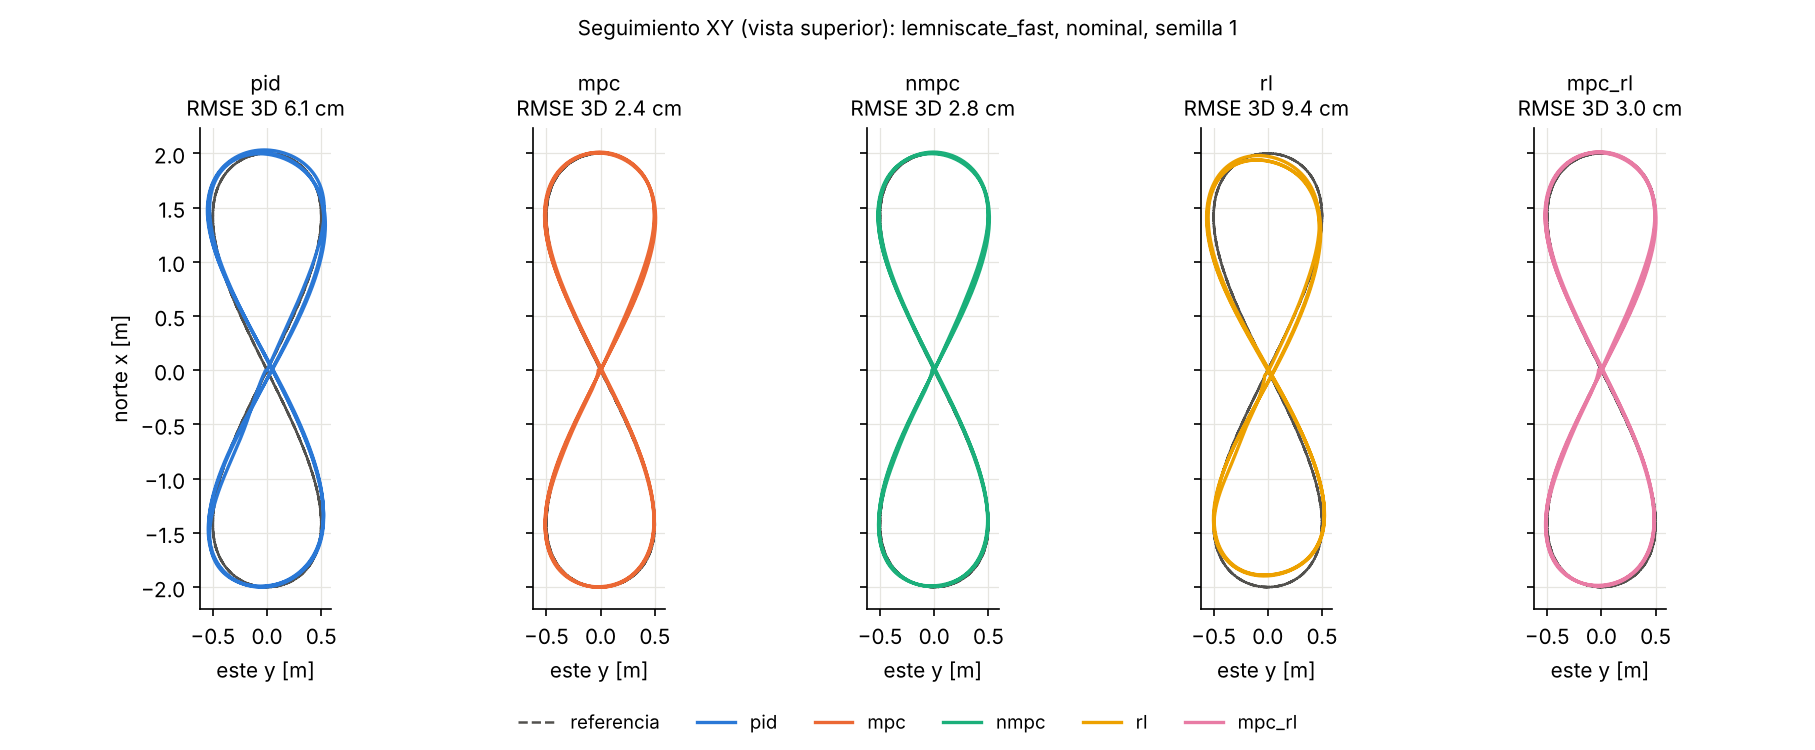
\includegraphics[width=\textwidth]{xy_lemniscate_fast_nominal.png}
\caption{Figura en 8 rápida, escenario nominal, semilla 1: trayectoria
horizontal de los cinco controladores sobre la referencia (banco final).}
\label{fig:xy}
\end{figure}

\begin{figure}[H]
\centering
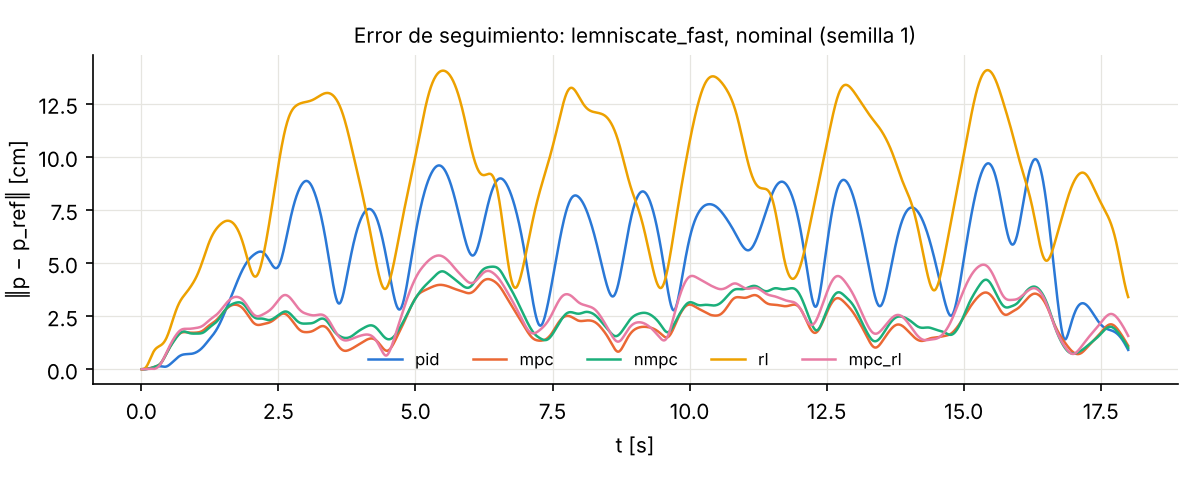
\includegraphics[width=\textwidth]{err_lemniscate_fast_nominal.png}
\caption{Norma del error de posición en la figura en 8 rápida, escenario
nominal, semilla 1 (banco final).}
\label{fig:err}
\end{figure}

\begin{table}[H]
\centering
\small
\caption{Trayectoria de escalones (caja de 1~m en XY y escalón de altura),
escenario nominal: métricas de escalón horizontal promediadas sobre los
escalones y las tres semillas. ``n/d'': no queda dentro de la banda del
2~\% antes del siguiente escalón.}
\label{tab:escalones}
\begin{tabular}{lccccc}
\toprule
 & PID & MPC & NMPC & RL puro & MPC+RL \\
\midrule
Sobreimpulso [\%] & \val{bpidstepwaypointsnominalos} & \val{bmpcstepwaypointsnominalos} & \val{bnmpcstepwaypointsnominalos} & \val{brlstepwaypointsnominalos} & \val{bmpcrlstepwaypointsnominalos} \\
Subida 10--90~\% [s] & \val{bpidstepwaypointsnominaltr} & \val{bmpcstepwaypointsnominaltr} & \val{bnmpcstepwaypointsnominaltr} & \val{brlstepwaypointsnominaltr} & \val{bmpcrlstepwaypointsnominaltr} \\
Establecimiento 2~\% [s] & \val{bpidstepwaypointsnominalts} & \val{bmpcstepwaypointsnominalts} & \val{bnmpcstepwaypointsnominalts} & \val{brlstepwaypointsnominalts} & \val{bmpcrlstepwaypointsnominalts} \\
Error final [cm] & \val{bpidstepwaypointsnominalss} & \val{bmpcstepwaypointsnominalss} & \val{bnmpcstepwaypointsnominalss} & \val{brlstepwaypointsnominalss} & \val{bmpcrlstepwaypointsnominalss} \\
\bottomrule
\end{tabular}
\end{table}

\subsection{Lectura del banco}
\label{sec:lectura_banco}

\paragraph{Qué permiten afirmar tres semillas.} En las filas de figura en 8
y círculo los rangos $\pm$ de MPC, NMPC y MPC+RL se solapan, de modo que la
tabla, leída columna contra columna, no separa a esos tres. La comparación
útil es por semilla, porque cada semilla da a todos los controladores el
mismo ruido, el mismo sesgo y la misma turbulencia. Con ese criterio el MPC
queda por debajo del PID en \val{pairMpcPid} de las \val{pairTotal} parejas
(fila $\times$ semilla) y por debajo del NMPC en todas las semillas de
\val{pairMpcNmpcRows} de las \val{nCombos} filas; el MPC+RL queda por
encima del MPC en \val{pairMpcrlWorse} de las \val{pairTotal}. Aun cuando
las tres semillas coinciden, una prueba de signos da $p=0.25$ (bilateral):
son tendencias consistentes, no diferencias estadísticamente probadas. Para
probarlas harían falta más semillas. Hay además un detalle de cálculo: la
validación de \cod{docs/RL.md} usó la desviación poblacional y este banco
la muestral, así que sus $\pm$ no se comparan directamente.

\paragraph{Controladores clásicos.} El MPC lineal tiene la media más baja en
\val{bestMpc} de las \val{nCombos} filas y el NMPC en \val{bestNmpc}. En la
figura en 8 rápida nominal el MPC reduce el error del PID en
\val{fastGain}~\%, porque anticipa la referencia en lugar de reaccionar a
ella. El NMPC cuesta unas \val{nmpcCost} veces más cómputo que el MPC sin
mejorarlo en las trayectorias suaves, por las razones de la sección
anterior. Hay que recordar la asimetría de la afinación: PID, MPC y NMPC se
afinaron con la semilla 1 de la figura en 8 y el círculo, que forma parte
de esta tabla.

\paragraph{Interferencia magnética en maniobra rápida.} Es la fila más
exigente del banco. \val{lostSentence} Los demás la sostienen, y su
resultado depende de una decisión de diseño del filtro de navegación. La
compuerta de innovación (\cref{sec:estimadores}) rechaza una medida de
posición solo si es improbable (más de 5 desviaciones estándar) \emph{y}
además grande (más de 25~cm, \cod{gate\_min\_m}). Con la interferencia, el
rumbo estimado se desvía y el acelerómetro se lleva al marco inercial con
un rumbo equivocado, así que la predicción del filtro queda sesgada. Frente a
un sensor de posición de 1~cm de ruido, una compuerta puramente estadística
descartaría entonces de forma sistemática medidas correctas y el filtro
derivaría: con ella, el MPC llega a 1.6~m de RMSE en esta fila; con el
piso, a \val{bmpclemniscatefastmagemi}~cm. En las trayectorias lentas con
interferencia la diferencia entre controladores es menor (el PID en la
figura en 8 da \val{bpidlemniscatemagemi}~cm, frente a
\val{bmpclemniscatemagemi}~cm del MPC); con los escalones de 1~m, en cambio,
el PID entra en el ciclo límite descrito antes
(\val{bpidstepwaypointsmagemi}~cm).

\paragraph{Aprendizaje por refuerzo.} El RL puro no alcanza al MPC: en
\val{rlRatioRows}, su RMSE medio va de \val{rlRatioMin} a \val{rlRatioMax}
veces el del MPC, y por semilla llega a \val{rlRatioSeedMax}. Tampoco es
siempre el peor: supera al PID en \val{rlBeatsPid} de las \val{nCombos}
filas (\val{rlBeatsPidList}).

La causa de la brecha está, sobre todo, en la política. En su propio
sustituto, sin aleatorizar, el RL puro ya comete 4.25~cm de RMSE en la
figura en 8, frente a 0.14~cm del MPC (\cod{validation\_gap\_ablation.json},
núcleo anterior); en esta tabla comete \val{brllemniscatenominal}~cm. Casi
todo el error ya existía donde se entrenó, y lo que falta en el
sustituto explica el resto. Cuáles dinámicas faltantes pesan más
(segundo orden del lazo de actitud, acoplamiento, ruido y retardo de la
posición, vibración) es por ahora una hipótesis: la comparación entre
sustituto y 6-DOF cambia todos esos factores a la vez y se hizo con el
núcleo anterior, con un sustituto que hoy, re-identificado, da otros
rezagos ($\approx$75~ms y 40~ms frente a 82.5 y 32~ms). El híbrido
aumenta el RMSE del MPC entre un \val{resMin} y un \val{resMax}~\% según la
fila; como se vio arriba, su residuo ya empeora al MPC dentro del sustituto.

\section{Barridos de parámetros y análisis de sensibilidad}
\label{sec:barridos}

Uno de los requisitos del proyecto es que los filtros también se sintonicen,
como se sintoniza un PID, y que el software barra sus parámetros de forma
automática. El
módulo \cod{quadsim/sweeps.py} (con \cod{objectives.py} y
\cod{experiments/sweep\_cli.py}) lo hace; el informe completo está en
\cod{docs/BARRIDOS.md}. Esta sección resume el método y los hallazgos que
tocan al modelo.

\subsection{Método}

{\sloppy Cada parámetro se nombra con una ruta de texto (\cod{filter.rp.0.fc},
\cod{estimator.ekf.accel\_noise}, \cod{pid.rp.rate\_kd\_scale},
\cod{sensors.vib\_gyro\_dps}, \ldots) que se aplica a la configuración o a la
simulación viva solo con su API pública. Los diseños de experimento son
grilla completa, aleatorio o hipercubo latino \cite{mckay79}, con
refinamiento local alrededor del mejor punto (paso exploratorio de Hooke y
Jeeves \cite{hooke61}). Hay tres ingredientes que vuelven útil la
comparación:\par}

\begin{itemize}
\item \textbf{Números aleatorios comunes} \cite{lawkelton}: la semilla
depende de la réplica y no del punto, así que todos los puntos ven el mismo
ruido, el mismo sesgo y la misma turbulencia; las diferencias entre puntos
vienen de los parámetros, y dos réplicas ya muestran tendencias limpias.
\item \textbf{Costo normalizado}, $J=\sum_kw_k\,m_k/m_k^{base}$, donde la base
es la configuración por defecto con las mismas semillas ($J<1$ es mejor que
el defecto), junto con el frente de Pareto de dos métricas, que es la
respuesta honesta cuando hay compromiso.
\item \textbf{Condiciones}: parámetros que son condiciones de operación
(vibración, EMI) y no ajustes. Cada punto se corre en todas y el ranking es
robusto (promedio o peor caso), para que el ``mejor'' punto no sea siempre
el de la condición más fácil.
\end{itemize}

Los escenarios de evaluación incluyen escalones de actitud y un
\emph{doblete de tasa} de $\pm90^\circ$/s, porque el retardo de un filtro casi
no se nota en el escalón de ángulo (el error de seguimiento varió entre
2.02 y $2.07^\circ$ con cortes de 20 a 200~Hz) y sí en la respuesta de tasa.
El ruido que llega a los motores se mide como el RMS del acelerador por
encima de 20~Hz en vuelo estacionario (\cod{motor\_hf\_pct}): un motor con
$T_m=20$~ms no sigue mandos más rápidos que unos 8~Hz, y esa energía se va
en calor. Es un sustituto, porque el modelo de motor no tiene pérdidas
eléctricas.

\subsection{Hallazgos que tocan al modelo}

\begin{itemize}
\item \textbf{La vibración está donde dice el modelo.} En todas las corridas
el tono dominante del giroscopio crudo está en 177.3--177.6~Hz, la
frecuencia de paso de pala calculada.
\item \textbf{Pasa-bajos: compromiso asimétrico.} Subir el corte de 80 a
200~Hz mejora el sobreimpulso de tasa 3.5 puntos pero multiplica por 13 el
ruido de motor; bajarlo a 20~Hz casi no quita más ruido y dispara el
sobreimpulso al 51~\%. Con el mismo corte, un $Q=1.2$ atrasa menos que
Butterworth.
\item \textbf{Notch.} Centrado en 178~Hz con $Q=1$ reduce el ruido de motor
63~\% con la mitad de retardo, y permite subir el pasa-bajos a 150~Hz. Un
notch angosto ($Q=8$) descentrado 2~Hz pierde casi todo su beneficio: es la
razón de los notch dinámicos ligados a las rpm.
\item \textbf{El derivativo SIMC era bajo.} Con $k_d=K_c\theta/3$ el doblete
de tasa tiene 20~\% de sobreimpulso; con el triple, 5.3~\%, con solo 7~\% más
de ruido de motor. Kd y corte del filtro deben moverse juntos: bajar el
corte a 40--60~Hz y subir $k_d$ de 3 a 4 veces da 3--6~\% de sobreimpulso
con 40--70~\% menos ruido.
\item \textbf{Estimadores.} El EKF con $\sigma_a=\sigma_m=0.05$ estaba mal
sintonizado: sin EMI, $(\sigma_a,\sigma_m)\approx(1.1,\,0.007)$ baja el error
de roll/pitch y de yaw 3 y 7 veces; el punto robusto frente a EMI es
$(0.5,\,0.3)$; $\beta$ de Madgwick óptimo entre
0.10 y 0.15; Mahony por defecto a 3~\% de su óptimo. Con EMI ninguna
ganancia arregla el rumbo: en Madgwick y Mahony el magnetómetro corrige los
tres ejes y contamina roll y pitch.
\item \textbf{Los barridos encuentran los huecos del costo.} Una primera
versión del costo sin el tiempo de establecimiento del ángulo llevó al
optimizador a bajar la ganancia de tasa y ``ganar'' con un dron lento; y
sintonizar el filtro solo en vuelo estacionario con turbulencia lleva a un
filtro excesivo (20~Hz). El escenario y el costo deben excitar la dinámica
que se quiere proteger.
\end{itemize}

\paragraph{Qué transfiere al dron real.} La forma de los compromisos, no los
números: la amplitud y el espectro de la vibración son supuestos. Antes de
transferir una sintonía de filtros hay que medir el espectro real del
giroscopio en hover, ajustar $A_g$ en el simulador hasta que el pico
coincida, y repetir el barrido.

\paragraph{Qué se aplicó al núcleo.} A partir de estos barridos y de la
verificación de este documento se cambiaron los valores por defecto: $k_d$ de
tasa de $K_c\theta/3$ a $K_c\theta$, pasa-bajos del giroscopio de 80 a 60~Hz,
ruidos del EKF a $(\sigma_a,\sigma_m)=(0.5,0.3)$, Butterworth de 30~Hz sobre el
acelerómetro antes del AHRS y estimador por defecto Mahony. Para $\beta$ de
Madgwick \emph{no} se tomó el óptimo del barrido (0.10--0.15) sino 0.015: el
barrido corría el estimador en sombra con el acelerómetro crudo, y en lazo
cerrado con el acelerómetro filtrado un $\beta$ grande produce un ciclo
límite (\cref{sec:estimadores}). Con los nuevos valores, el escenario
\cod{attitude\_step} pasó de 20.1 a 5.9~\% de sobreimpulso de tasa y de
0.78 a 0.43$^\circ$ de error de estimación con Madgwick (0.51$^\circ$ con
Mahony); en \cod{estimator\_accuracy} el error RMS bajó de 0.70 a 0.63$^\circ$
con Mahony y de 1.14 a 0.68$^\circ$ con el EKF, cuyo error de rumbo pasó de
2.55 a 0.43$^\circ$. Las tablas de \cod{docs/BARRIDOS.md} se produjeron con
el núcleo anterior.

\paragraph{Barridos de estimadores: sombra y vuelo.} Los barridos de
\cod{madgwick\_beta}, \cod{mahony\_gains} y \cod{ekf\_noise} corren el
estimador candidato en sombra. Hasta la revisión de octubre de 2026 esa
cadena no era la que se vuela: recibía el acelerómetro sin el Butterworth
previo al AHRS y una aceleración cinemática calculada por un filtro de
navegación alimentado con el estimador ideal, sin el lazo autorreferente de
la \cref{sec:leishman}. La revisión externa midió 1.26$^\circ$ RMS en sombra
frente a 0.43$^\circ$ en el lazo para Madgwick. Hoy la sombra y el vuelo usan
la misma función (\cod{quadsim/estimation.py}); los resultados de esos
barridos en \cod{docs/BARRIDOS.md} se obtuvieron con la cadena anterior, y
por eso el $\beta$ por defecto se decidió con mediciones en lazo cerrado y
no con el óptimo del barrido.

\section{Limitaciones y trabajo futuro}
\label{sec:limitaciones}

Un modelo se defiende mejor declarando sus límites que escondiéndolos. Esta
sección separa lo que se omitió a sabiendas, con su justificación, de lo que
se detectó durante la verificación o en la revisión externa y sigue
abierto, y termina con los datos del dron real que hacen falta para cerrar
varios de esos puntos.

\subsection{Omisiones del modelo físico}

\begin{itemize}
\item \textbf{Dinámica eléctrica del motor y reacción por aceleración del
rotor.} El propulsor de primer orden no satura la corriente, por lo que su
aceleración inicial ante un escalón es irreal y el término $-\dot{\vect h}_r$
se omite (\cref{sec:reaccion}). Un modelo con resistencia de devanado,
constante $K_t$ y límite de corriente permitiría incluirlo y daría además
una medida directa de calentamiento, en lugar del sustituto
\cod{motor\_hf\_pct}.
\item \textbf{Constante de tiempo del motor.} $T_m=20$~ms viene de
CopterSim, no de los motores del proyecto, y es la misma en todo punto de
operación, con carga o sin ella, al acelerar y al frenar, sin límite de
pendiente. El lazo de tasa es más sensible a $T_m$ que a los retardos
omitidos: con 30~ms el margen de fase baja de 58.7 a 48.1$^\circ$
(\cref{sec:integracion}).
\item \textbf{Batería.} Voltaje constante: $C_R$ no cae durante el vuelo y
el acelerador de hover no deriva. CopterSim trae un modelo de batería que
podría portarse.
\item \textbf{Aerodinámica del rotor.} No hay \emph{blade flapping}, arrastre
inducido ni pérdida de empuje en vuelo de avance, que a velocidades de
varios m/s producen fuerzas horizontales y momentos de cabeceo
proporcionales a la velocidad. Tampoco hay anillo de vórtices en descensos
rápidos. El arrastre vertical es un supuesto y el momento del arrastre por
la separación de 0.12~m entre centro aerodinámico y de masa que declara
CopterSim no se modela.
\item \textbf{Efecto suelo.} Escala el empuje de cada rotor pero no su par
de arrastre. Es un supuesto de modelado, no una consecuencia del modelo de
efecto suelo elegido.
\item \textbf{Forma del empuje.} $T=C_T\Omega^2$ puro, frente al ajuste
$b\Omega^2+a\Omega+c$ que Quitian Niño \cite{quitian22} encontró
significativo en banco.
\item \textbf{Inercia y carga.} Tensor diagonal; la carga útil no agrega
productos de inercia y su desplazamiento vertical del centro de masa no
produce brazo para el empuje.
\item \textbf{Turbulencia.} Filtros de primer orden en los tres ejes,
alineados con NED (\cref{sec:perturbaciones}).
\item \textbf{Suelo.} Restricción simple sin fricción ni rebote.
\end{itemize}

\subsection{Omisiones de la cadena digital}

\begin{itemize}
\item \textbf{ESC.} Por defecto responde de forma instantánea y continua a
$\sigma$: no hay frecuencia de PWM, protocolo (PWM, OneShot, DShot) ni
filtrado de entrada. Con PWM de 50~Hz el margen de fase del lazo de tasa
caería a 39.6$^\circ$ y la ganancia admisible a 2.4 veces
(\cref{tab:margenes}). Las opciones \cod{esc\_rate\_hz} y
\cod{esc\_pulse\_delay\_s} permiten estudiarlo, pero el valor real del dron
del proyecto no se conoce todavía.
\item \textbf{Retardo de cómputo.} Por defecto el mando se aplica en el
mismo periodo en que se calcula; \cod{compute\_delay\_samples} agrega uno o
más periodos. Su efecto sobre los márgenes está en la
\cref{sec:integracion}.
\item \textbf{Resolución del acelerador.} $\sigma$ es continuo por defecto.
Con el LEDC del ESP32 a 50~Hz y 10 bits quedan unos 51 escalones útiles,
que pueden generar ciclos límite; \cod{throttle\_levels} permite
cuantizarlo.
\item \textbf{Temporización ideal.} El lazo es perfectamente periódico: no
hay \emph{jitter} de FreeRTOS (interrupciones de la radio NRF24 o del WiFi,
lecturas I2C), ni desfase entre la tasa de salida de la IMU y el lazo de
500~Hz, ni el filtro digital interno de la IMU. El retardo de 2~ms de la IMU
es un supuesto sin fuente citada.
\item \textbf{Barómetro.} Un ruido de 0.17~m corresponde a un modo de alta
resolución del BMP180, cuya conversión limita la tasa a unos 13--33~Hz; la
simulación usa 40~Hz. Falta contrastarlo con la hoja de datos y con la
configuración del firmware.
\item \textbf{Enlace de posición.} Además del retardo de 10~ms del sensor,
\cod{pos\_link\_delay\_s} suma la latencia del enlace (captura de movimiento
o radio, típicamente 5--30~ms). Vale 0 por defecto porque depende del
sistema de posicionamiento que se use con el dron real.
\end{itemize}

Los valores por defecto de las opciones nuevas (\cod{compute\_delay\_samples},
\cod{esc\_rate\_hz}, \cod{esc\_pulse\_delay\_s}, \cod{throttle\_levels},
\cod{pos\_link\_delay\_s}) conservan el
comportamiento con el que se identificaron los rezagos y se afinaron los
controladores, para que las cifras de este documento sigan siendo
reproducibles. Una sintonía hecha con ellas desactivadas es optimista en
margen de fase. Antes de llevarla al dron conviene repetir el escalón de
tasa con los valores reales del ESC y del firmware.

\subsection{Hallazgos de la verificación}

Varios hallazgos de la verificación ya se corrigieron en el núcleo y este
documento describe el estado corregido: el pasa-bajos del acelerómetro antes
del AHRS, que elimina el sesgo de inclinación por rectificación de la
vibración (de \val{rectmadC} a \val{rectmadF}$^\circ$ con Madgwick); el
arranque en el aire coherente (líneas de retardo llenas, AHRS alineado,
covarianza de navegación en régimen); el filtro que se rediseña en vuelo
sin transitorio; los valores por defecto de $k_d$, del filtro del
giroscopio, del EKF y de $\beta$. La revisión externa de octubre de 2026
llevó a corregir además: la compensación de aceleración, que ya no se aplica
sin correcciones horizontales de posición absoluta, entra en rampa, se
recorta y pasa por el mismo filtro que el acelerómetro
(\cref{sec:leishman}); la corrección magnética de Madgwick y Mahony, que
ahora solo actúa sobre el rumbo; la base de tiempo con razones no enteras
entre física y control (\cref{sec:integracion}); la línea de retardo de los
sensores, que ahora admite retardo nulo y fraccional y arranca cebada; la
validación de nombres de estimadores y de ganancias, que antes ignoraba sin
aviso una clave mal escrita; el tope del integrador de Mahony; el registro,
que ya no descarta columnas que aparecen a mitad de corrida; y una
regularización adaptativa en el iLQR del NMPC. Quedan abiertos:

\begin{itemize}
\item \textbf{Compensación de aceleración.} Con sensor de posición sigue
siendo autorreferente entre correcciones y queda un desfase de unos 17~ms
entre las dos señales que se restan (\cref{sec:leishman}). Sin sensor de
posición queda desactivada, así que en ese modo el AHRS vuelve a
equivocarse durante las aceleraciones sostenidas. La solución de fondo es
un filtro de navegación con el error de actitud como estado.
\item \textbf{Error de actitud en ángulos de Euler.} El lazo de ángulo resta
ángulos de Euler. Es válido con el límite de 30$^\circ$, pero se degrada en
maniobras agresivas y es singular cerca de $\pm90^\circ$ de cabeceo; PX4
usa el error de cuaternión.
\item \textbf{Madgwick sin estimación de sesgo.} El término de compensación
de deriva del artículo original no está implementado; la comparación con
Mahony y el EKF, que sí estiman el sesgo, debe leerse con eso en mente.
\item \textbf{Retardo de la cadena en la sintonía.} Las ganancias por
defecto se calculan con la cadena nominal ($\theta=16.0$~ms); la cadena
configurada, con filtros, cómputo y ESC, solo se usa con
\cod{gains\_from\_chain} (\cref{sec:control}). Ninguna de las dos incluye
el filtro del derivativo ni la fase exacta del motor.
\item \textbf{Barridos de estimadores anteriores.} Las tablas de
\cod{docs/BARRIDOS.md} se obtuvieron con la cadena de sombra anterior, que
no era la que se vuela (\cref{sec:barridos}); habría que repetirlos.
\item \textbf{Rezagos y políticas sin regenerar.} \cod{DEFAULT\_LAGS}, los
pesos del MPC y del NMPC y las políticas de RL se obtuvieron con el núcleo
anterior (Madgwick, sin filtro de acelerómetro); no se volvieron a
identificar, afinar ni entrenar (\cref{sec:posicion}). Re-identificar el
sustituto hoy da otros rezagos, así que la receta de \cod{docs/RL.md} no
reproduce exactamente los archivos de \cod{models/}.
\item \textbf{Ciclo límite del PID con EMI en escalones.} Incluso con
$K_{i,xy}=2$ (\cref{sec:posicion}).
\item \textbf{Exponente de la EMI.} $\sigma^{1.5}$ no se deriva del modelo de
propulsor (\cref{sec:perturbaciones}).
\item \textbf{Fusión del barómetro con el sensor de posición activo.} Inocua
en la práctica, pero no intencional (\cref{sec:estimadores}).
\end{itemize}

\subsection{Alcance del banco de controladores}

\begin{itemize}
\item \textbf{Tres semillas.} Bastan para ver tendencias consistentes, no
para probar diferencias de milímetros (\cref{sec:lectura_banco}).
\item \textbf{Afinación sobre el conjunto de prueba.} PID, MPC y NMPC se
afinaron con la semilla 1 de la figura en 8 y el círculo, que forma parte
del banco, y el integral del PID se eligió mirando el caso con EMI. El RL no
tuvo esa ventaja.
\item \textbf{Aprendizaje por refuerzo.} Un solo entrenamiento PPO por
política, cortado cuando la curva todavía bajaba; previsión, observación,
salida y límite de inclinación distintos de los del MPC; validación con
trayectorias que pertenecen a la familia de entrenamiento; y un residuo
elegido por costo y no por error. Las conclusiones valen para estas
políticas, no para el RL en general.
\end{itemize}

\subsection{Datos pendientes del dron real}

Cuatro mediciones cerrarían buena parte de lo anterior:
\begin{enumerate}
\item protocolo y frecuencia de actualización del ESC del dron (PWM,
OneShot o DShot, y su tasa);
\item constante de tiempo del motor medida en banco, con escalones de
acelerador y tacómetro óptico, en subida y en bajada;
\item modo y tasa reales del BMP180 en el firmware;
\item sistema de posicionamiento disponible (captura de movimiento, RTK o
ninguno) y su latencia, que decide si la compensación de aceleración puede
usarse y cuánto retardo tiene la posición.
\end{enumerate}

\subsection{Trabajo futuro}

El paso que más valor agrega es medir el dron real del proyecto y
reemplazar los parámetros de la literatura: masa y brazo, $C_T$ y $C_M$ en
banco, la recta del ESC y $T_m$ con escalones, inercias con péndulo
compuesto y trifilar (el protocolo de Quitian Niño \cite{quitian22}, de esta
misma universidad, ya describe esos bancos), y el espectro de vibración en
hover. Con esos números y los datos pendientes de arriba, el flujo que este
documento verifica (identificar los rezagos, derivar ganancias SIMC, afinar
en simulación con barridos y validar con el banco) se repite sobre el
vehículo real. Para los controladores de aprendizaje el orden es el
contrario del que sugería la edición anterior: primero mejorar la política
(observaciones normalizadas, la misma previsión que el MPC, salida como
corrección sobre la aceleración de referencia, selección por error de
validación y varias semillas de entrenamiento) y después, con una ablación
de un factor a la vez, decidir qué le falta al sustituto.

\clearpage
\phantomsection
\addcontentsline{toc}{section}{Referencias}
\begin{thebibliography}{99}
\small
\setlength{\itemsep}{0.25em}

\bibitem{qq17} Quan, Q. (2017). \emph{Introduction to Multicopter Design and
Control}. Springer, Singapur. (Caps.~4, 5 y 6: propulsor, marcos y modelo
dinámico.)

\bibitem{qq20} Quan, Q., Dai, X. y Wang, S. (2020). \emph{Multicopter Design
and Control Practice: A Series Experiments Based on MATLAB and Pixhawk}.
Springer, Singapur. ISBN 978-981-15-3137-8.

\bibitem{cs19} Dai, X. CopterSim, archivo \texttt{Init.m}. Repositorio
\texttt{github.com/XunhuaDai/CopterSim}, commit \texttt{0d14487f} (25 de julio
de 2019). Consultado el 4 de octubre de 2026.

\bibitem{hb16} Powers, C., Mellinger, D. y Kumar, V. (2015). Quadrotor
kinematics and dynamics. En K.~P. Valavanis y G.~J. Vachtsevanos (eds.),
\emph{Handbook of Unmanned Aerial Vehicles}, cap.~16, pp.~307--328. Springer.

\bibitem{hb11} Phang, S.~K., Li, K., Chen, B.~M. y Lee, T.~H. (2015).
Systematic design methodology and construction of micro aerial quadrotor
vehicles. En \emph{Handbook of Unmanned Aerial Vehicles}, cap.~11,
pp.~181--206. Springer.

\bibitem{jirinec11} Jiřinec, T. (2011). \emph{Stabilization and Control of
Unmanned Quadcopter}. Tesis de maestría, Czech Technical University in
Prague.

\bibitem{luukkonen11} Luukkonen, T. (2011). \emph{Modelling and Control of
Quadcopter}. Independent research project, Aalto University School of
Science, Espoo.

\bibitem{quitian22} Quitian Niño, L.~C. (2022). \emph{Construcción de bancos
de prueba para la medición experimental de los parámetros del modelo
dinámico de drones -- UAS}. Tesis de maestría, Universidad Nacional de
Colombia, Bogotá.

\bibitem{larotta24} Larotta Mariño, L.~A. (2024). \emph{Control de posición
para un cuadricóptero basado en un sistema de realidad virtual}. Tesis de
maestría, Universidad Nacional de Colombia, Bogotá.

\bibitem{madgwick11} Madgwick, S.~O.~H., Harrison, A.~J.~L. y
Vaidyanathan, R. (2011). Estimation of IMU and MARG orientation using a
gradient descent algorithm. \emph{IEEE International Conference on
Rehabilitation Robotics (ICORR)}.

\bibitem{mahony08} Mahony, R., Hamel, T. y Pflimlin, J.-M. (2008). Nonlinear
complementary filters on the special orthogonal group. \emph{IEEE
Transactions on Automatic Control}, 53(5), 1203--1218.

\bibitem{sabatini06} Sabatini, A.~M. (2006). Quaternion-based extended
Kalman filter for determining orientation by inertial and magnetic sensing.
\emph{IEEE Transactions on Biomedical Engineering}, 53(7), 1346--1356.

\bibitem{leishman14} Leishman, R.~C., Macdonald, J.~C., Beard, R.~W. y
McLain, T.~W. (2014). Quadrotors and accelerometers: State estimation with
an improved dynamic model. \emph{IEEE Control Systems Magazine}, 34(1),
28--41.

\bibitem{skogestad03} Skogestad, S. (2003). Simple analytic rules for model
reduction and PID controller tuning. \emph{Journal of Process Control},
13(4), 291--309.

\bibitem{astrom04} Åström, K.~J. y Hägglund, T. (2004). Revisiting the
Ziegler--Nichols step response method for PID control. \emph{Journal of
Process Control}, 14(6), 635--650.

\bibitem{mellinger11} Mellinger, D. y Kumar, V. (2011). Minimum snap
trajectory generation and control for quadrotors. \emph{IEEE International
Conference on Robotics and Automation (ICRA)}, 2520--2525.

\bibitem{richter13} Richter, C., Bry, A. y Roy, N. (2013). Polynomial
trajectory planning for aggressive quadrotor flight in dense indoor
environments. \emph{International Symposium of Robotics Research (ISRR)}.

\bibitem{cheeseman55} Cheeseman, I.~C. y Bennett, W.~E. (1955). The effect
of the ground on a helicopter rotor in forward flight. \emph{Aeronautical
Research Council, Reports and Memoranda} No.~3021.

\bibitem{mil8785} U.S. Department of Defense (1980). \emph{MIL-F-8785C:
Flying Qualities of Piloted Airplanes}.

\bibitem{milhdbk1797} U.S. Department of Defense (1997). \emph{MIL-HDBK-1797:
Flying Qualities of Piloted Aircraft}.

\bibitem{rbj} Bristow-Johnson, R. \emph{Cookbook formulae for audio EQ
biquad filter coefficients} (``Audio EQ Cookbook''). Documento técnico de
amplia circulación, publicado por la W3C como nota de grupo de trabajo.

\bibitem{ism330} STMicroelectronics. \emph{ISM330DHCX: iNEMO inertial module,
3D accelerometer and 3D gyroscope}. Hoja de datos DS13012.

\bibitem{mmc5983} MEMSIC. \emph{MMC5983MA: 3-axis magnetic sensor}. Hoja de
datos.

\bibitem{bmp180} Bosch Sensortec. \emph{BMP180 digital pressure sensor}. Hoja
de datos BST-BMP180-DS000.

\bibitem{uiuc} Brandt, J.~B., Deters, R.~W., Ananda, G.~K., Dantsker, O.~D. y
Selig, M.~S. \emph{UIUC Propeller Database}. University of Illinois at
Urbana-Champaign.

\bibitem{hairer93} Hairer, E., Nørsett, S.~P. y Wanner, G. (1993).
\emph{Solving Ordinary Differential Equations I: Nonstiff Problems}, 2.ª ed.
Springer.

\bibitem{landau76} Landau, L.~D. y Lifshitz, E.~M. (1976). \emph{Mechanics},
3.ª ed. (Course of Theoretical Physics, vol.~1). Pergamon.

\bibitem{beck09} Beck, A. y Teboulle, M. (2009). A fast iterative
shrinkage-thresholding algorithm for linear inverse problems. \emph{SIAM
Journal on Imaging Sciences}, 2(1), 183--202.

\bibitem{odonoghue15} O'Donoghue, B. y Candès, E. (2015). Adaptive restart
for accelerated gradient schemes. \emph{Foundations of Computational
Mathematics}, 15(3), 715--732.

\bibitem{pannocchia03} Pannocchia, G. y Rawlings, J.~B. (2003). Disturbance
models for offset-free model-predictive control. \emph{AIChE Journal},
49(2), 426--437.

\bibitem{maeder09} Maeder, U., Borrelli, F. y Morari, M. (2009). Linear
offset-free model predictive control. \emph{Automatica}, 45(10),
2214--2222.

\bibitem{li04} Li, W. y Todorov, E. (2004). Iterative linear quadratic
regulator design for nonlinear biological movement systems.
\emph{International Conference on Informatics in Control, Automation and
Robotics (ICINCO)}.

\bibitem{tassa12} Tassa, Y., Erez, T. y Todorov, E. (2012). Synthesis and
stabilization of complex behaviors through online trajectory optimization.
\emph{IEEE/RSJ International Conference on Intelligent Robots and Systems
(IROS)}.

\bibitem{tassa14} Tassa, Y., Mansard, N. y Todorov, E. (2014).
Control-limited differential dynamic programming. \emph{IEEE International
Conference on Robotics and Automation (ICRA)}.

\bibitem{diehl05} Diehl, M., Bock, H.~G. y Schlöder, J.~P. (2005). A
real-time iteration scheme for nonlinear optimization in optimal feedback
control. \emph{SIAM Journal on Control and Optimization}, 43(5),
1714--1736.

\bibitem{torrente21} Torrente, G., Kaufmann, E., Föhn, P. y Scaramuzza, D.
(2021). Data-driven MPC for quadrotors. \emph{IEEE Robotics and Automation
Letters}, 6(2), 3769--3776.

\bibitem{sun22} Sun, S., Romero, A., Foehn, P., Kaufmann, E. y Scaramuzza, D.
(2022). A comparative study of nonlinear MPC and differential-flatness-based
control for quadrotor agile flight. \emph{IEEE Transactions on Robotics},
38(6), 3357--3373.

\bibitem{schulman17} Schulman, J., Wolski, F., Dhariwal, P., Radford, A. y
Klimov, O. (2017). Proximal policy optimization algorithms.
arXiv:1707.06347.

\bibitem{johannink19} Johannink, T., Bahl, S., Nair, A., Luo, J., Kumar, A.,
Loskyll, M., Ojea, J.~A., Solowjow, E. y Levine, S. (2019). Residual
reinforcement learning for robot control. \emph{IEEE International
Conference on Robotics and Automation (ICRA)}.

\bibitem{silver18} Silver, T., Allen, K., Tenenbaum, J. y Kaelbling, L.
(2018). Residual policy learning. arXiv:1812.06298.

\bibitem{tobin17} Tobin, J., Fong, R., Ray, A., Schneider, J., Zaremba, W. y
Abbeel, P. (2017). Domain randomization for transferring deep neural
networks from simulation to the real world. \emph{IEEE/RSJ IROS}.

\bibitem{mckay79} McKay, M.~D., Beckman, R.~J. y Conover, W.~J. (1979). A
comparison of three methods for selecting values of input variables in the
analysis of output from a computer code. \emph{Technometrics}, 21(2),
239--245.

\bibitem{hooke61} Hooke, R. y Jeeves, T.~A. (1961). ``Direct search''
solution of numerical and statistical problems. \emph{Journal of the ACM},
8(2), 212--229.

\bibitem{lawkelton} Law, A.~M. y Kelton, W.~D. \emph{Simulation Modeling and
Analysis}. McGraw-Hill (cap. sobre técnicas de reducción de varianza:
números aleatorios comunes).

\end{thebibliography}

\end{document}
